\section{Matrix Element Method}\label{sec:mem}

In this section we describe the Matrix Element Method (MEM) for the $t\bar{t}H$ multilepton analysis.

\subsection{The algorithm}

The matrix element method consists in estimating the probability of an event to be compatible with the signal or background hypothesis, by computing the cross section of signal or background processes on a given phase-space point, corresponding to the reconstructed kinematic configuration of the event.

For each hypothesis $\alpha$, a weight $w_{i,\alpha}$ is computed for the event $i$ using the following formula:
\begin{displaymath}
w_{i,\alpha}(\Phi ') = \frac{ 1 }{ \sigma_{\alpha}} \int d\Phi_{\alpha} \cdot  \delta^4 \Big( p_1^{ \mu}+p_2^{ \mu} - \sum_{k\geq 2}p_k^{ \mu} \Big) \cdot  \frac{  f(x_1,\mu_F) f(x_2,\mu_F) }{ x_1 x_2 s } \cdot \Big| \mathcal{M}_{\alpha} ( p_k^{ \mu} ) \Big|^2 \cdot W(\Phi '| \Phi_{\alpha})
\end{displaymath}

where $\sigma_{\alpha}$ is the cross section of the process $\alpha$, $\Phi '$ is the 4-momenta of the reconstructed particles in the event, $d\Phi_{\alpha}$  are the process-dependent integration variables, corresponding to the 4-momenta of all the particles at the vertex in the hypothesis $\alpha$, the $\delta$ symbol represents the momentum conservation between incoming and final state particles, $f(x,\mu_F)$ are the parton density function in the proton, $x_1$, $x_2$ are the fraction of proton energy carried by the incoming particles, $\Big| \mathcal{M}_{\alpha} ( p_k^{ \mu} ) \Big|^2$ is the matrix element squared, and $W$ are the transfer functions relating the energy of particles at the vertex with their energy reconstructed with the detector.

The MEM for $t\bar{t}H$ multilepton analysis is implemented in C++, thus can be easily intefaced with analysis code. The integration is performed using VEGAS \cite{VEGAS} stratified/importance sampling implementation in ROOT. The matrix element squared is taken from Madgraph standalone C++ code at LO. The parton distribution functions are taken from LHAPDF6 \cite{Buckley:2014ana}. Transfer functions are evaluated in CMS Run II Monte Carlo simulation. The phase space is analytic and implemented as in Madweight \cite{Artoisenet:2010cn}.

\subsubsection*{$t\bar{t}H$, and $t\bar{t}V$ and $t\bar{t}$ hypotheses}

In this analysis, the MEM for two lepton same-sign, three leptons and four leptons categories are considered.
Hypotheses corresponding to $t\bar{t}H$ signal (with semi-leptonic and fully leptonic Higgs decay), and $t\bar{t}W$, $t\bar{t}\gamma^{*}/Z$ irreducible backgrounds, and $t\bar{t}$ reducible backgrounds (semi-leptonic and fully leptonic top decay) are included.

For all of the three processes, the $W$ mass for $W$ arising from top and Higgs decays is not treated as fixed, and follows a Breit-Wigner as specified by the matrix element squared.
The $W$ and $\gamma^{*}/Z$ bosons produced in association with $t\bar{t}$ in $t\bar{t}V$ processes are also following a Breit Wigner. Interference between $\gamma^{*}$ and $Z$ is included in the $t\bar{t}\gamma^{*}/Z$ matrix element.

On the other hand, to decrease the number of integration variables, the masses of the top quark and Higgs bosons are set to 173 GeV and 125 GeV respectively. In this narrow-width approximation, matrix element and phase-space of top, anti-top and Higgs/$W$/$Z$ can be computed independently:

\begin{displaymath}
\Big| \mathcal{ M_{\alpha}}   \Big|^2 = \Big| \mathcal{ M}_{TTH}   \Big|^2 \cdot  \Big| \mathcal{ M}_{Top}\Big|^2 \cdot  \Big| \mathcal{ M}_{Antitop}  \Big|^2 \cdot  \Big| \mathcal{ M}_{Higgs}  \Big|^2
\end{displaymath}
\begin{displaymath}
d\Phi_{tot} = d\Phi_{gg\rightarrow TTH} \cdot d\Phi_{Top} \cdot d\Phi_{Antitop} \cdot d\Phi_{Higgs}
\end{displaymath}

The phase-space $d\Phi_{\alpha}$ is made of the product of all final state particle $dE d\theta d\phi$. Integration over some of these variables can be cancelled using momentum conservation formula.
We implemented the phase-space parametrization proposed in Madweight MEM paper. This was compared with a custom parametrization and found to be faster. Changes of variables are performed to make explicit the $W$ mass, which follows always a Breit Wigner and do not depends on event kinematics, such that VEGAS can treat it as an independent variable. We reproduce here the integration variables which are used:
\begin{displaymath}
d\Phi_{top,had}  \propto dE_b  d\theta_b d\phi_b \cdot d\theta_{j1} d\phi_{j1}  \cdot  d\theta_{j2} d\phi_{j2} \cdot dm_{W}
\end{displaymath}
\begin{displaymath}
d\Phi_{top,lep}  \propto dE_b  d\theta_b d\phi_b \cdot dE_l d\theta_l d\phi_l  \cdot d\phi_{\nu} dm_{W}
\end{displaymath}
\begin{displaymath}
d\Phi_{H\rightarrow 2l2\nu}  \propto dE_{l1}  d\theta_{l1} d\phi_{l1} \cdot  dE_{l2}  d\theta_{l2} d\phi_{l2} \cdot dE_{\nu1} d\theta_{\nu1} d\phi_{\nu1} \cdot d\phi_{\nu2} dm_{W2}
\end{displaymath}
\begin{displaymath}
d\Phi_{H\rightarrow l\nu jj}  \propto  dE_{j1} d\theta_{j1} d\phi_{j1}  \cdot  dE_{j2}  d\theta_{j2} d\phi_{j2} \cdot  dE_{l1}  d\theta_{l1} d\phi_{l1}  \cdot  d\phi_{\nu1} dm_{W1}
\end{displaymath}
\begin{displaymath}
d\Phi_{Z}  \propto dE_{l1}  d\theta_{l1} d\phi_{l1}  \cdot  dE_{l2}  d\theta_{l2} d\phi_{l2}
\end{displaymath}
\begin{displaymath}
d\Phi_{W}  \propto dE_{l}  d\theta_{l} d\phi_{l}   \cdot d\theta_{\nu}  d\phi_{\nu}   dm_{W}
\end{displaymath}

For a given value of the integration variables, the momenta of all particles can be computed by solving a set of linear and quadratic equations.
The $b$-quark mass is set to 4.7 GeV while the masses of the non-b quarks and leptons is set to 0.

The matrix element squared provided by Madgraph is leading order in pQCD, i.e. with no additional jets recoiling against the $t\bar{t}H/V$ system. However additional jets are present in data. To evalute the ME, the $t\bar{t}H/V$ system needs to be boosted back along the $Px/Py$ direction such that the incoming particles have no $Px/Py$ component.

The pdf chosen is NNPDF2.3 LO QED. The factorization scale in the pdf and matrix element are chosen to be $\mu_F =  (m_{t} + m_{H})/2$ for $t\bar{t}H$, $\mu_F =  (m_{t} + m_{W})/2$ for $t\bar{t}W$, and $\mu_F =  (m_{t} + m_{\gamma^{*}/Z})/2$ for $t\bar{t}\gamma^{*}/Z$.


\subsection{Treatment of jets and permutations}

To evaluate the matrix element, leptons, jets and b-jets need to be assigned to the ME leptons and quarks.
The jets assigned to the two b-quarks from tops are the two reconstructed jets with highest CSV value (disregarding the analysis categories 1b tight / 2b loose).

If all the needed jets are reconstructed, one has to choose 4 (2) jets among the remaining jets in two lepton same-sign (three lepton) category.
In the general case, the jets to be assigned to the ME will arise from $W$ decay from top or Higgs. For this reason, we select the dijet pair with mass closest to $m_W$.
In the three lepton categories, when attempting to evaluate the $t\bar{t}H, H\rightarrow l\nu jj$ hypothesis, the dijet pair can also arise from $W^{*}$ decay. Here we choose the dijet pair with lowest dijet mass (dijet mass is bounded by the $p_T$ cut on the jets to be mostly greater than 50 GeV). Similarly in two lepton same-sign categories, once the jet pair with mass closest to $m_W$ are selected, two more jets with lowest dijet mass are selected. It was shown that this "mixed" way of selecting jets performs better than selecting only jet pairs by mass closest to $W$ mass.

If the needed jets are not all reconstructed (e.g. not passing jet identification or escaping detector acceptance), in principle the matrix element can not be evaluated. However, by expanding the phase-space with additional integration variables for the missing jets, it is possible to circonvene this difficulty. This feature is implemented in the 1-missing and 2-missing jets cases. Thus the MEM can be computed for all events selected with the baseline analysis, requiring $\geq 4 (2)$ jets including b-jets, in 2lss (3l) category.

Since we cannot know a priori what is the correct lepton and jet assignment to the ME partons, the ME is evaluated for all possible permutations of leptons and jets. %Table \ref{mem:permutations} summarizes the number of permutations for all categories and hypotheses.

%\begin{table}
%\begin{center}
%\begin{tabular}{|c|c|c|c|c|c|}
%\hline
%Category/Hypothesis & $t\bar{t}Z$ & $t\bar{t}W$ & $t\bar{t}H,H\rightarrow l\nu jj$ & $t\bar{t}H,H\rightarrow 2l2\nu $ & $t\bar{t}H$ \\
%\hline
%\hline
%3l\_2b\_2j   & 4 or 8 & 4 & 8  & 8 & 16\\
%\hline
%3l\_2b\_1j   & 4 or 8 & 4 & 8  & 8 & 16\\
%\hline
%3l\_2b\_0j   & 2 or 4 & 4 & 4  & 4 & 8\\
%\hline
%4l\_2b       & 4 or 8 & 0 & 0  & 8 & 8\\
%\hline
%2lss\_2b\_4j & 0      & 8 & 96 & 0 & 96\\
%\hline
%2lss\_2b\_3j & 0      & 8 & 8 & 0 & 8\\
%\hline
%2lss\_2b\_2j & 0      & 8 & 4 & 0 & 4\\
%\hline
%\end{tabular}
%\caption{\label{mem:permutations}Number of permutations of all hypotheses and categories}
%\end{center}
%\end{table}

For all hypotheses and categories, there are 2 permutations arising from b-jet permutation (top or anti-top). If only one b-jet is selected, the permutation still needs to be done with the tops exchanging absence or presence of the b-jet.

The $t\bar{t}Z$ hypothesis can be computed in 3l (with 1 lepton from leptonic decay and 2 leptons from $Z$ decay) and 4l categories (2 leptons from both leptonic top decay and 2 leptons from $Z$ decay). In 3l/4l categories, there can be 1 or 2 same flavour opposite sign pair to make a $Z$, thus 1 or 2 lepton permutations are allowed, the other lepton(s) being assigned to the top/anti-top according to the sign of their charge. In 3l categories, 2 jet permutations are arising from the hadronic top decay.

The $t\bar{t}W$ ME does not have quarks in 3l categories (2 leptons from leptonic top decay and 1 lepton from associated W production), thus no jet permutations are allowed. In 2lss categories, 2 jets among 4 can be assigned to the ME (from a hadronic top decay), leading to 2 jet permutations in any case.

The $t\bar{t}H,H\rightarrow 2l2\nu $ hypothesis can be computed for 3l (with one leptonic top decay) and 4l categories (two leptonic top decays) only.

The $t\bar{t}H,H\rightarrow l\nu jj$ hypothesis can be computed for 2lss (with one hadronic top decay) and 3l (both leptonic top decays). The biggest number of permutations is found in the $2lss\_2b\_4j$ category, where permutations have to be done within the 4 jets. To reduce the number of permutations in the special case of $2lss\_2b\_3j$ category (time consuming since there are more integration variables) the missing jet can only be assigned to the $W$ from Higgs decay, assuming that the jet is lost because of not passing the $p_T$ requirement.

The $t\bar{t}$ hypothesis is splitted in semi-leptonic and fully leptonic top decay. In that case, the lepton permutation needs to be done while there are more reconstructed leptons available (2 same sign or 3) than in the matrix element (1 for semi-leptonic and 2 for fully leptonic).

Once the MEM is computed for each of the permutations, an average weight is computed for each hypothesis. The weights with null value are excluded from the average (found to be sligthly more discriminating than including them):
\begin{displaymath}
\left\{
  \begin{array}{lcl}
    w_{\alpha} = 10^{-300} \qquad \qquad \qquad \mathrm{ if } \sum w_i=0 \\
    w_{\alpha} = \frac{1}{N_{w_{i} \neq 0}} \sum_{w_{i} \neq 0} w_i  \qquad \mathrm{ else }\\
  \end{array}
\right.
\end{displaymath}


\subsubsection*{Transfer functions}

The transfer functions $W(\Phi '| \Phi_{\alpha})$ give the probability density of measuring a set of observables $\Phi '$ with the detector, given a phase space point $\Phi_{\alpha}$ at ME level. For this analysis, the following approximations are made. The lepton energy and its direction is assumed to be perfectly measured. The direction of quarks is assumed to be perfectly measured by the direction of the reconstructed jet. Thus no transfer functions are used for leptons, while jet energy transfer functions are included in the MEM.

Jets and b-jets energy transfer functions are evaluated in MC simulation with $CMSSW\_7\_6_\_X$. The pdfs are histograms parameterized as a function of $E_{rec}/E_{gen}$, where $E_{rec}$ is the jet reconstructed energy after jet energy scale/resolution correction and $E_{gen}$ is the energy of the matched parton. Transfer functions are defined in 3 bins of jet pseudorapidity ($|\eta| < 0.8$, $0.8 < |\eta| < 1.6$, $1.6 < |\eta| < 2.4$) and 6 bins of jet energy ($25 < E < 50$, $50 < E < 80$, $80 < E < 120$, $120 < E < 200$, $200 < E < 300$, $E > 300$ GeV).
B-jet response is found to be slightly lower than jet response, as expected (due to missing momentum of neutrinos from B-hadron decays escaping detection).
Transfer functions measured in $t\bar{t}H$ samples are used. Distributions were cross-checked in $t\bar{t}V$ and $t\bar{t}$ samples and found to behave similarly. Examples of jets and b-jets transfer functions are shown fig.~\ref{mem:JetsTF}.

\begin{figure}[Htb]
 \centering
   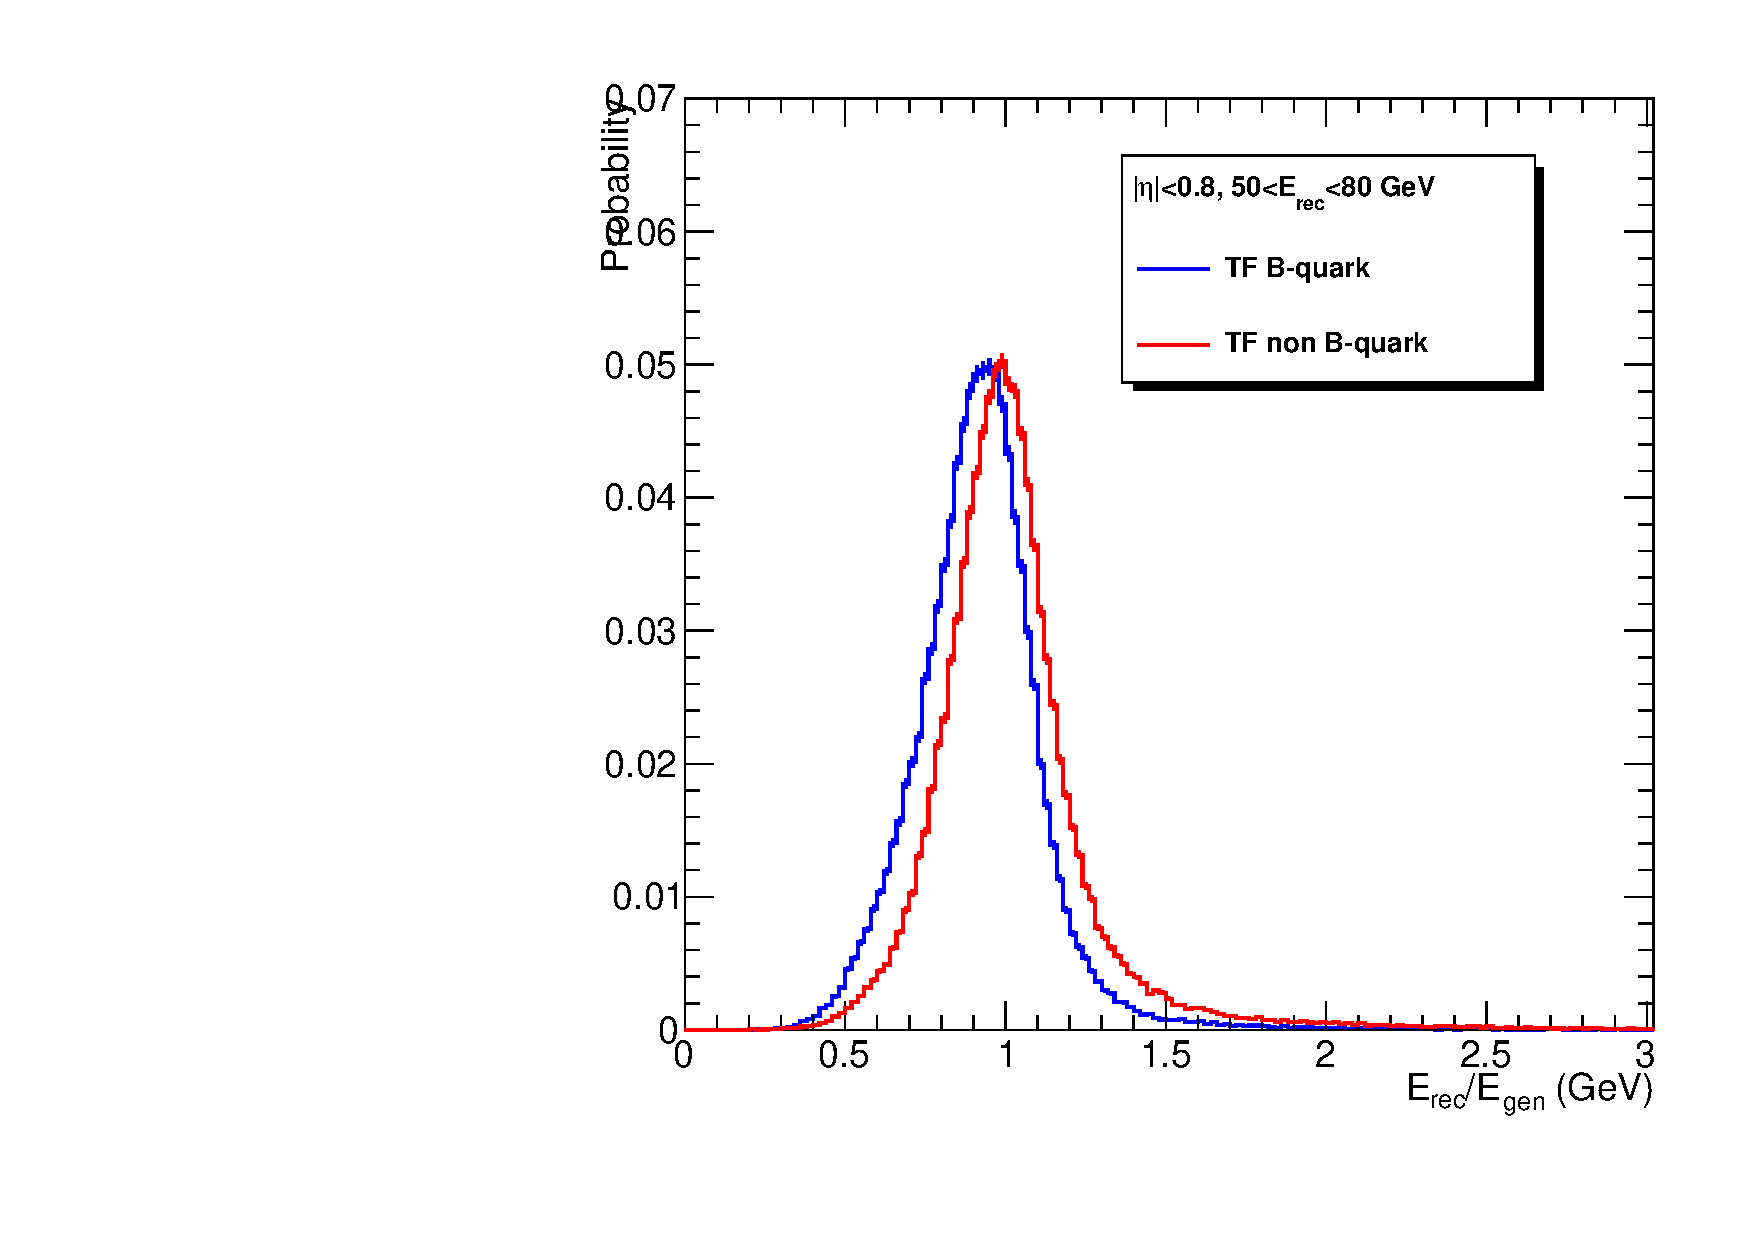
\includegraphics[width=0.4\textwidth]{plots_mem/TFratio_BnonB_Eta08_E50to80.pdf}\\
   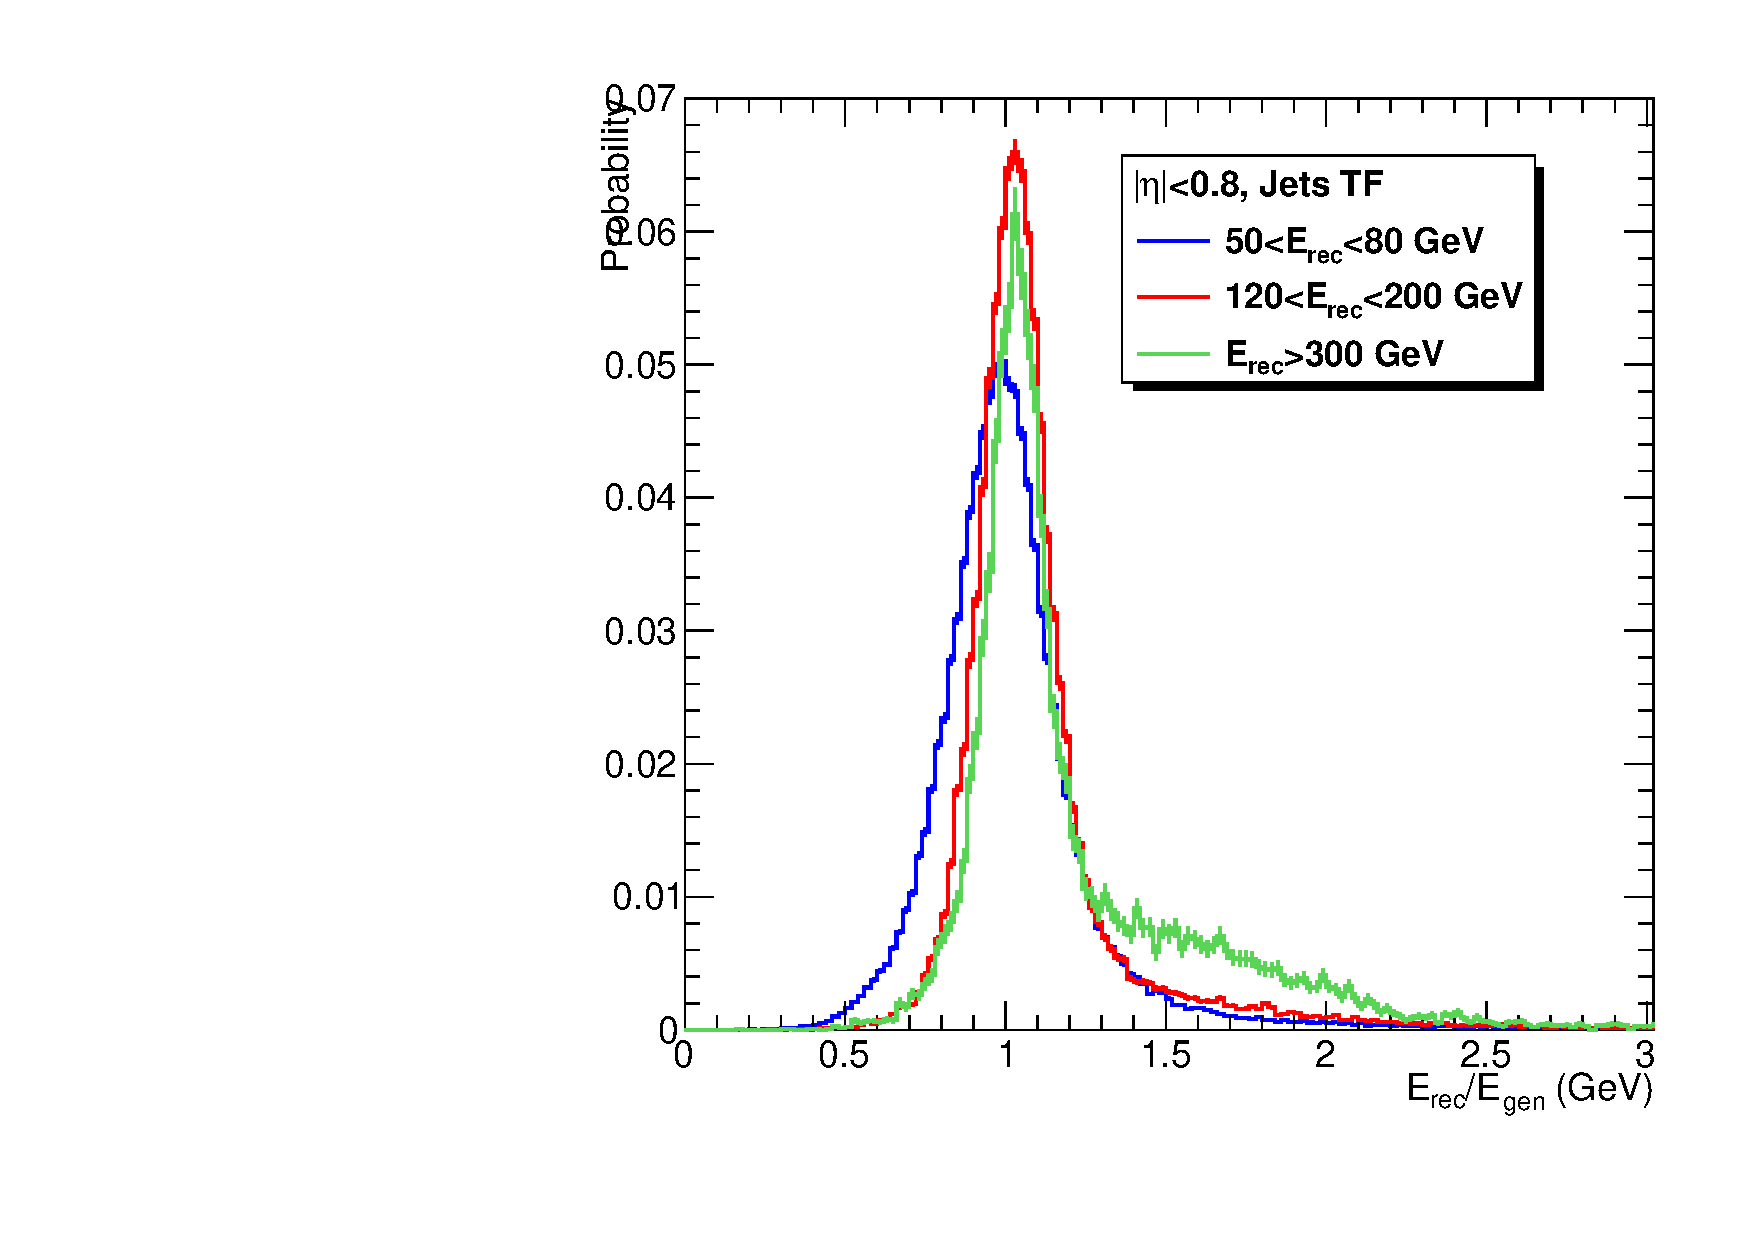
\includegraphics[width=0.4\textwidth]{plots_mem/TFratio_nonB_Eta08_varyEnergy.pdf}
   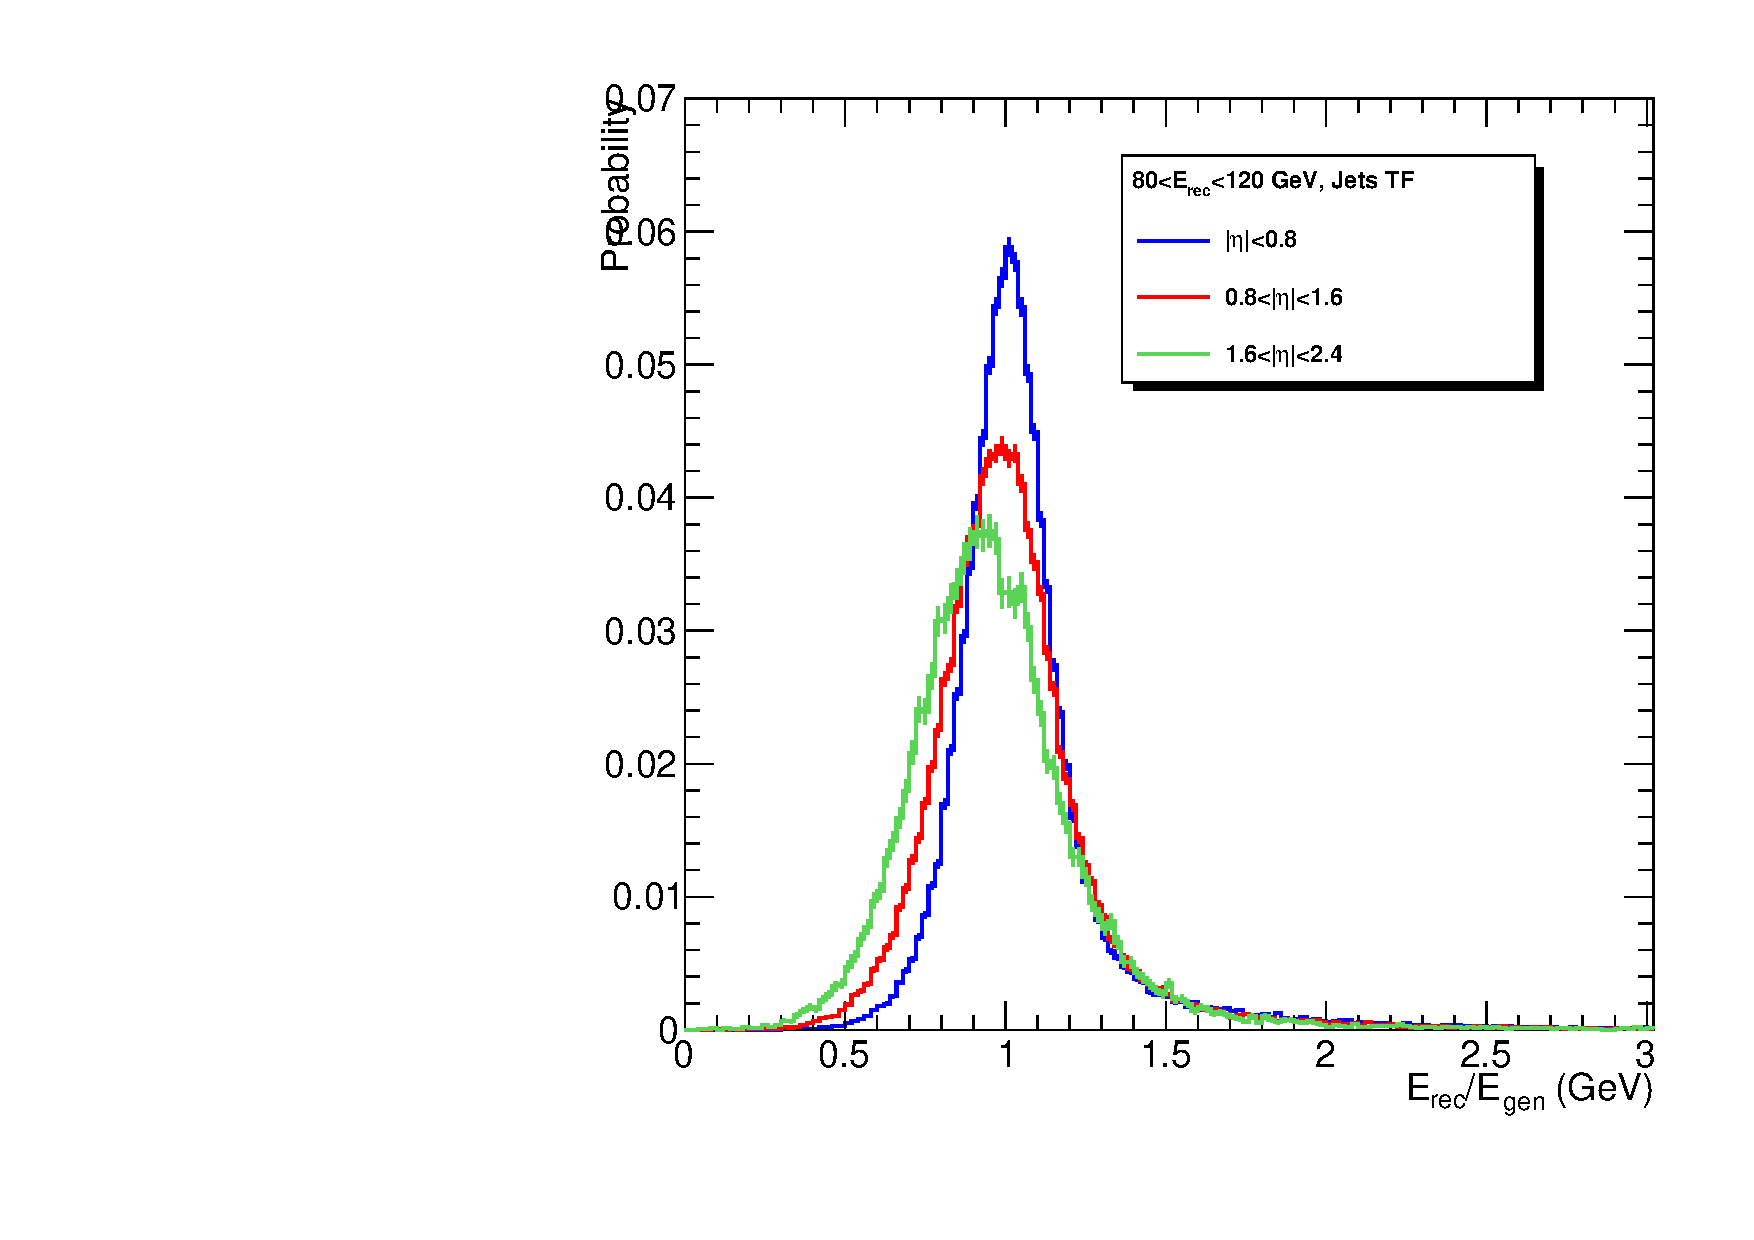
\includegraphics[width=0.4\textwidth]{plots_mem/TFratio_nonB_80E120_varyEta.pdf}
   \caption{Example of jets transfer functions for (a) b-jets and non-b jets, (b) variation of jets TF with energym (c) variation of jets TF with $\eta$.}
  \label{mem:JetsTF}

\end{figure}

If a jet is missing at reconstructed level, its transfer function is set to 0 if the associated MEM quark has $|\eta|>2.4$, and to 1 if $|\eta|<2.4$.

Another set of transfer functions is used to constrain the total momentum of the $t\bar{t}H/V$ system.
According to momentum conservation between intial state and final state particles, integration over the phase space of initial particles is cancelled.
Despite the cancellation, one can constrain the total momentum computed with the MEM at parton level with the total momentum reconstructed, by using a transfer function. For pratical reason, this transfer function is approximated with a missing transverse energy transfer function.
The parameterization is using the $mET$ and $mET$ $\phi$ distributions.
%The parameterization is using the $mET$ covariance matrix $|V_{x,y}|$ computed event by event to build a 2D pdf, as a function of $mET$ $Px$ and $Py$:
%\begin{displaymath}
%TF(E_x^{miss}, E_y^{miss})  = \frac{1}{2\pi \sqrt{|V_{x,y}|}}  exp \Big( -\frac{1}{2} (\overrightarrow{E_T}^{miss} - \sum{\overrightarrow{\nu_T}})^{T} V_{x,y}^{-1} (\overrightarrow{E_T}^{miss} - \sum{\overrightarrow{\nu_T}}) \Big)
%\end{displaymath}

\subsection{MEM discriminant}

According to the Neyman-Person lemma, the likelihood of signal and background is the most powerful test statistic for hypothesis testing. In the 2lss categories, a likelihood is built with the $t\bar{t}H$ and $t\bar{t}W$ hypotheses, while in the 3l categories, a likelihood is built with $t\bar{t}H$ and $t\bar{t}W$+$t\bar{t}Z$ hypotheses as follows:

\begin{displaymath}
L_{2lss} = - log \Big( \frac{ \sigma_{\mathrm{TTW}}w_{\mathrm{TTW}}}{\sigma_{\mathrm{TTH}}w_{\mathrm{TTH}} + k \cdot \sigma_{\mathrm{TTW}}w_{\mathrm{TTW}} } \Big)
\end{displaymath}

\begin{displaymath}
\left\{
  \begin{array}{lcl}
L_{3l} = -log \Big( \frac{ \sigma_{\mathrm{TTZ}}w_{\mathrm{TTZ}}+ k \cdot \sigma_{\mathrm{TTW}}w_{\mathrm{TTW}}}{\sigma_{\mathrm{TTH}}w_{\mathrm{TTH}} + \sigma_{\mathrm{TTZ}}w_{\mathrm{TTZ}} + k \cdot \sigma_{\mathrm{TTW}}w_{\mathrm{TTW}}} \Big)  \qquad \qquad \mathrm{  SFOS}  \\

L_{3l} = -log \Big( \frac{ k \cdot \sigma_{\mathrm{TTW}}w_{\mathrm{TTW}}}{\sigma_{\mathrm{TTH}}w_{\mathrm{TTH}} + k \cdot\sigma_{ \mathrm{TTW}}w_{\mathrm{TTW}} } \Big)   \qquad\qquad\qquad \qquad \mathrm{ no \quad SFOS}  \\
  \end{array}
\right.
\end{displaymath}

\begin{displaymath}
L_{4l} = - log \Big( \frac{ \sigma_{\mathrm{TTZ}}w_{\mathrm{TTZ}}}{\sigma_{\mathrm{TTH}}w_{\mathrm{TTH}} + \sigma_{\mathrm{TTZ}}w_{\mathrm{TTZ}} } \Big)
\end{displaymath}

MEM weights are weighted by relevant process cross section in the likelihood. Note that the $t\bar{t}Z$ hypothesis can be included only if there is at least one same flavour opposite sign pair to build a $Z$.

A multiplicative factor $k$ is included to counterbalance the missing phase space in the $t\bar{t}W$ hypothesis with respect to the other processes (the $t\bar{t}W$ ME has 2 jets less in the matrix element relative to $t\bar{t}H$ and $t\bar{t}Z$). In the case of 3l categories, $k$ was tuned for each category (0/1/2 missing jets) to maximize the signal to background discrimination. In the 2lss categories, changing $k$ does not improve discrimination but allows easier fit of the final distributions.

Final yields after event selection in $CMSSW\_7\_6\_X$ MC with 2015 luminosity assumed, are shown fig.~\ref{mem:memyields2lss} for 2lss categories fig.~\ref{mem:memyields3l} for 3l categories.

\begin{figure}[Htb]
 \centering
   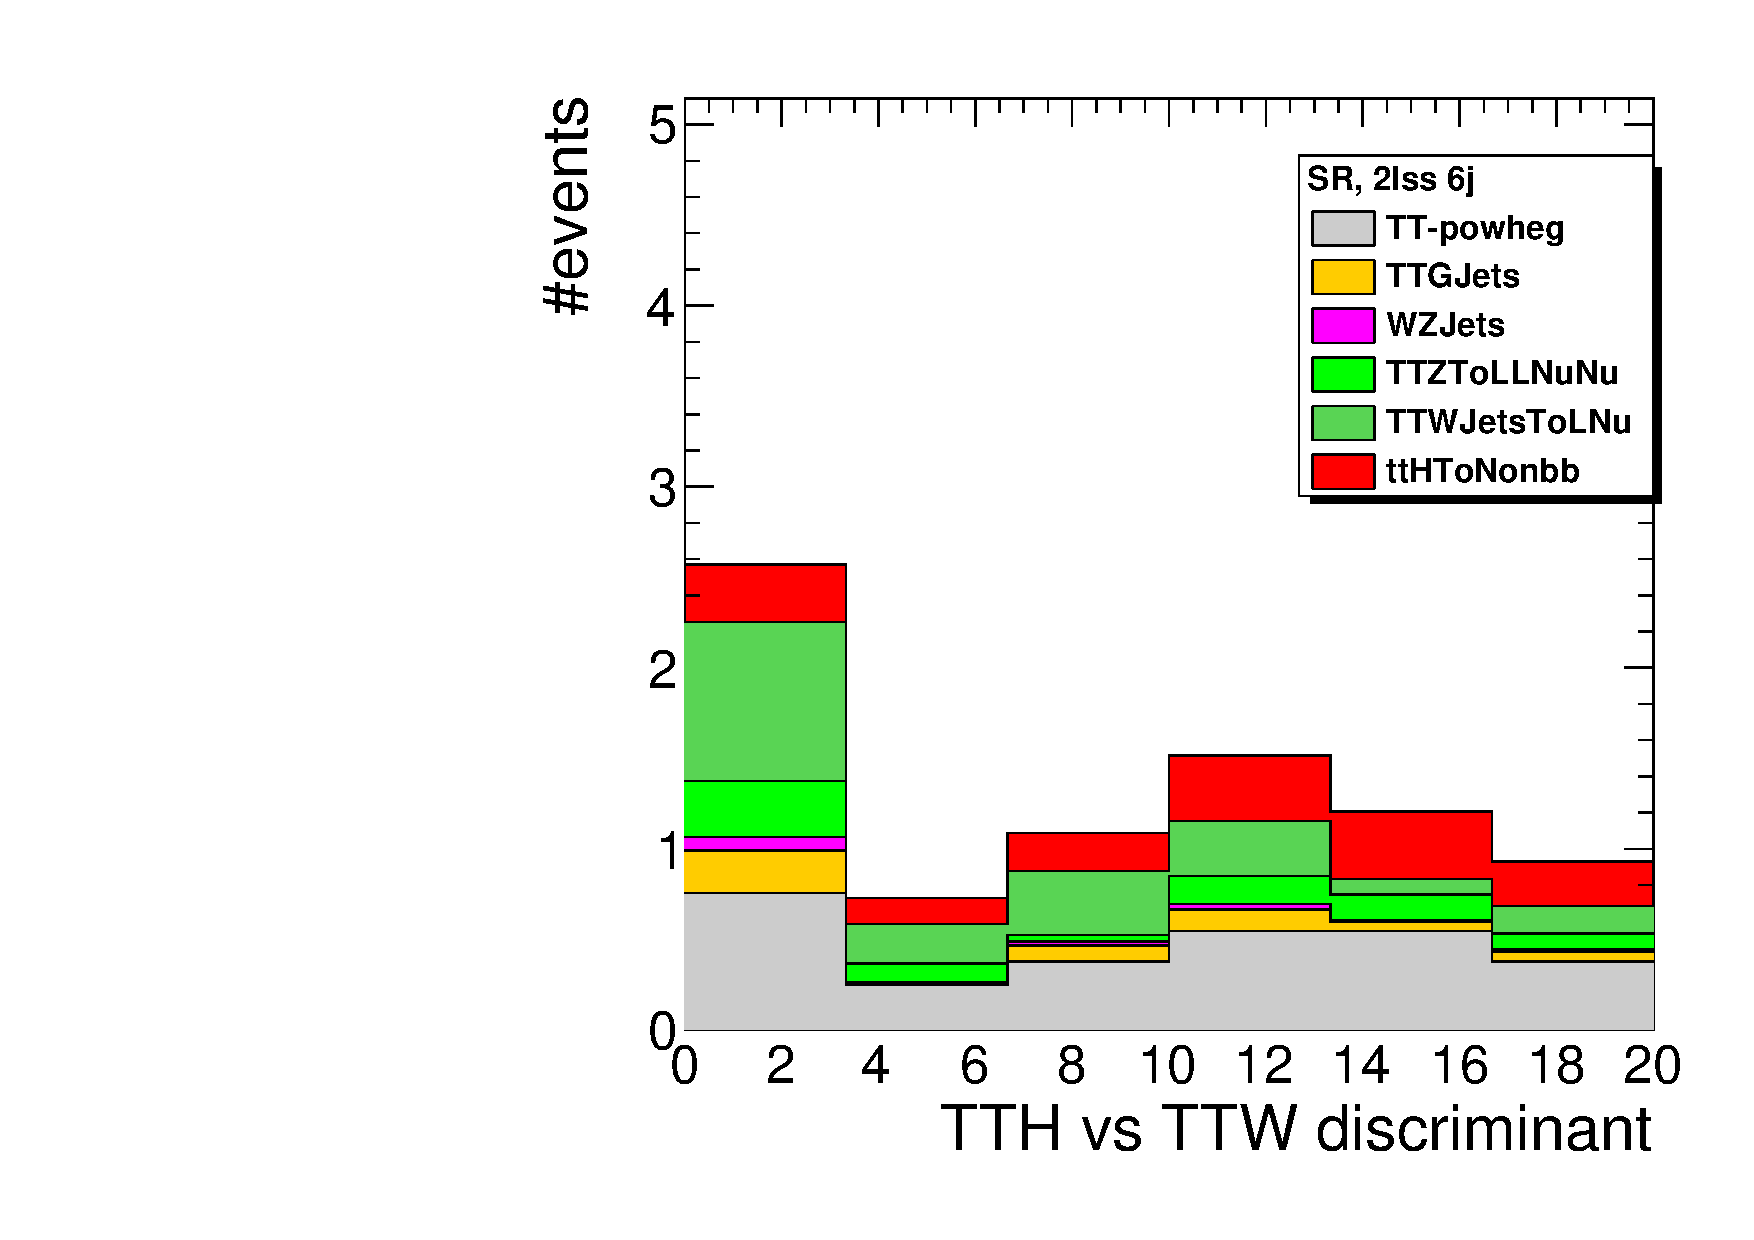
\includegraphics[width=0.4\textwidth]{plots_mem/Stack_MEMdiscriminant_2lss_SR_TTHvsTTVfull_miss0j.pdf}\\
   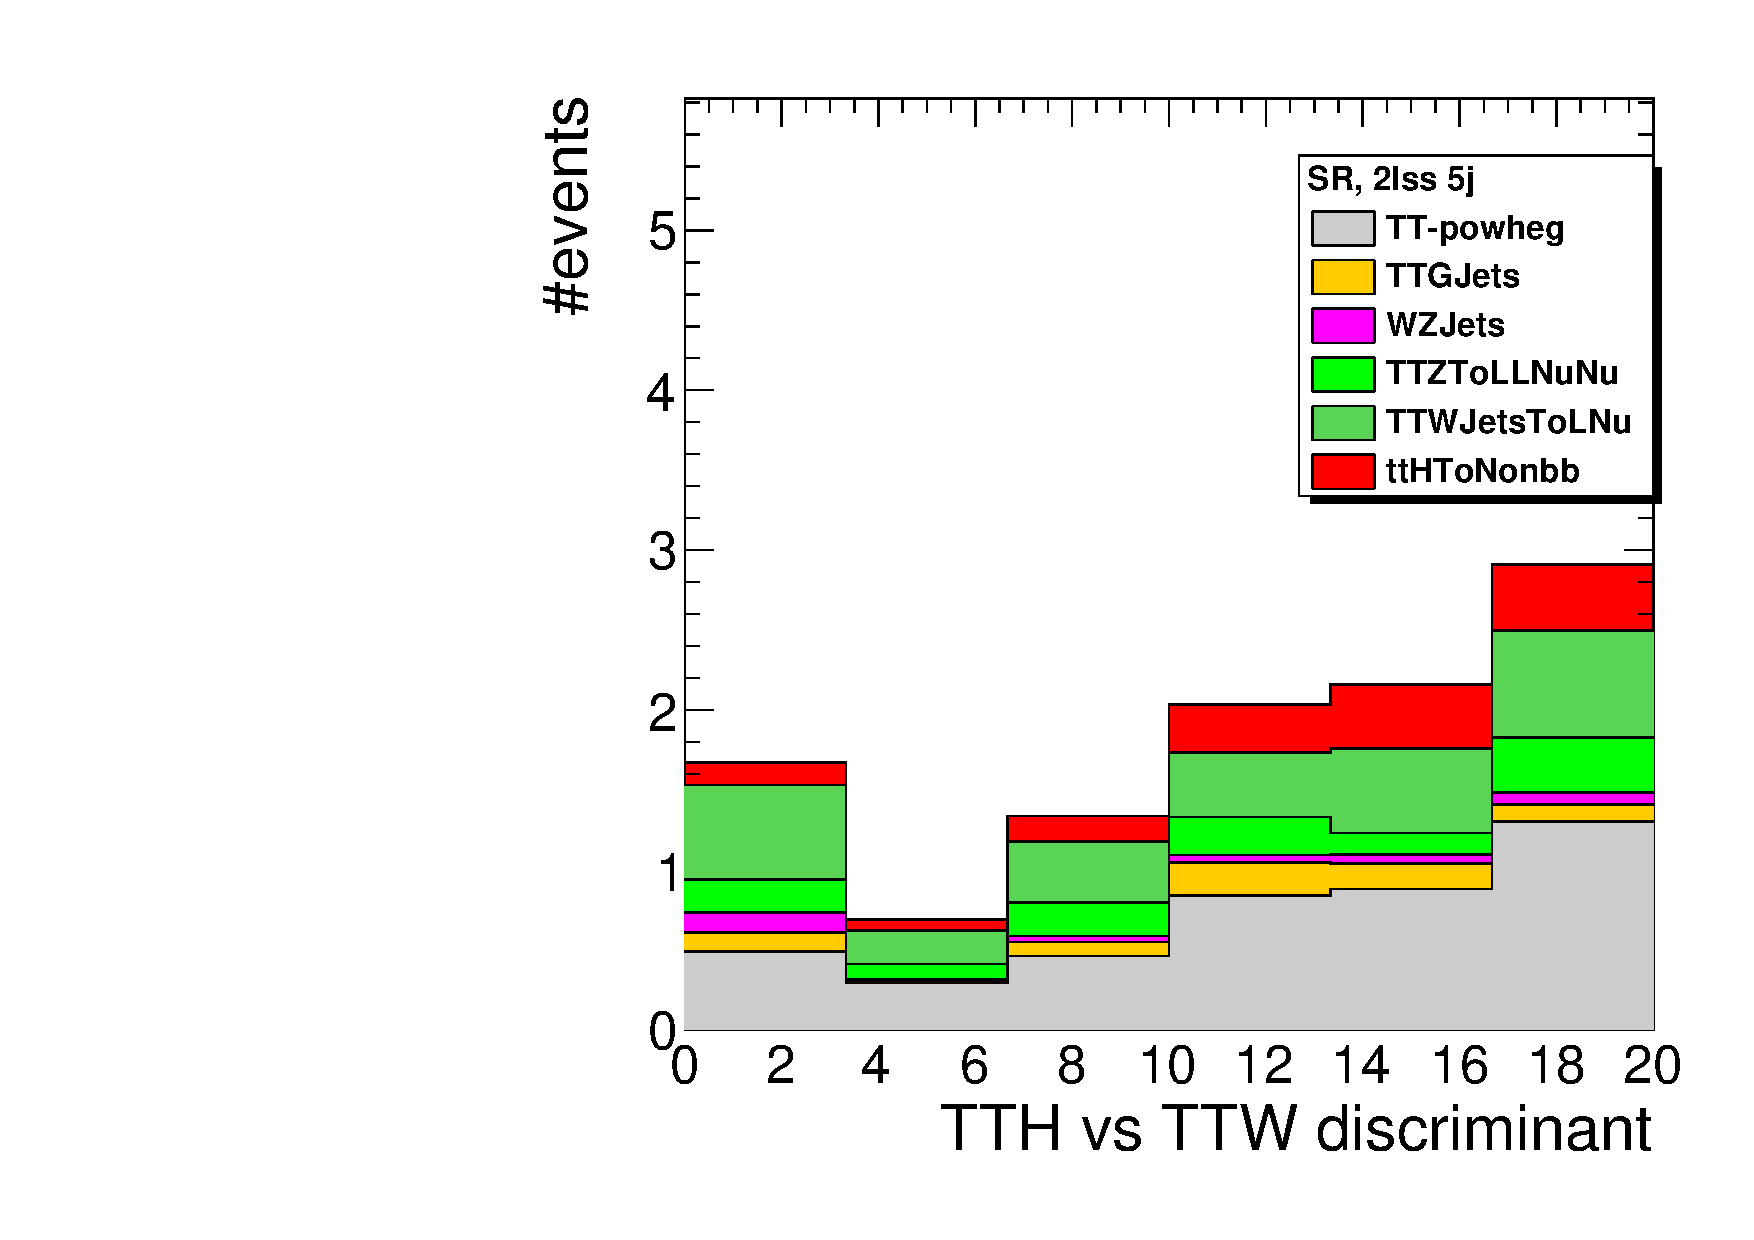
\includegraphics[width=0.4\textwidth]{plots_mem/Stack_MEMdiscriminant_2lss_SR_TTHvsTTVfull_miss1j.pdf}
   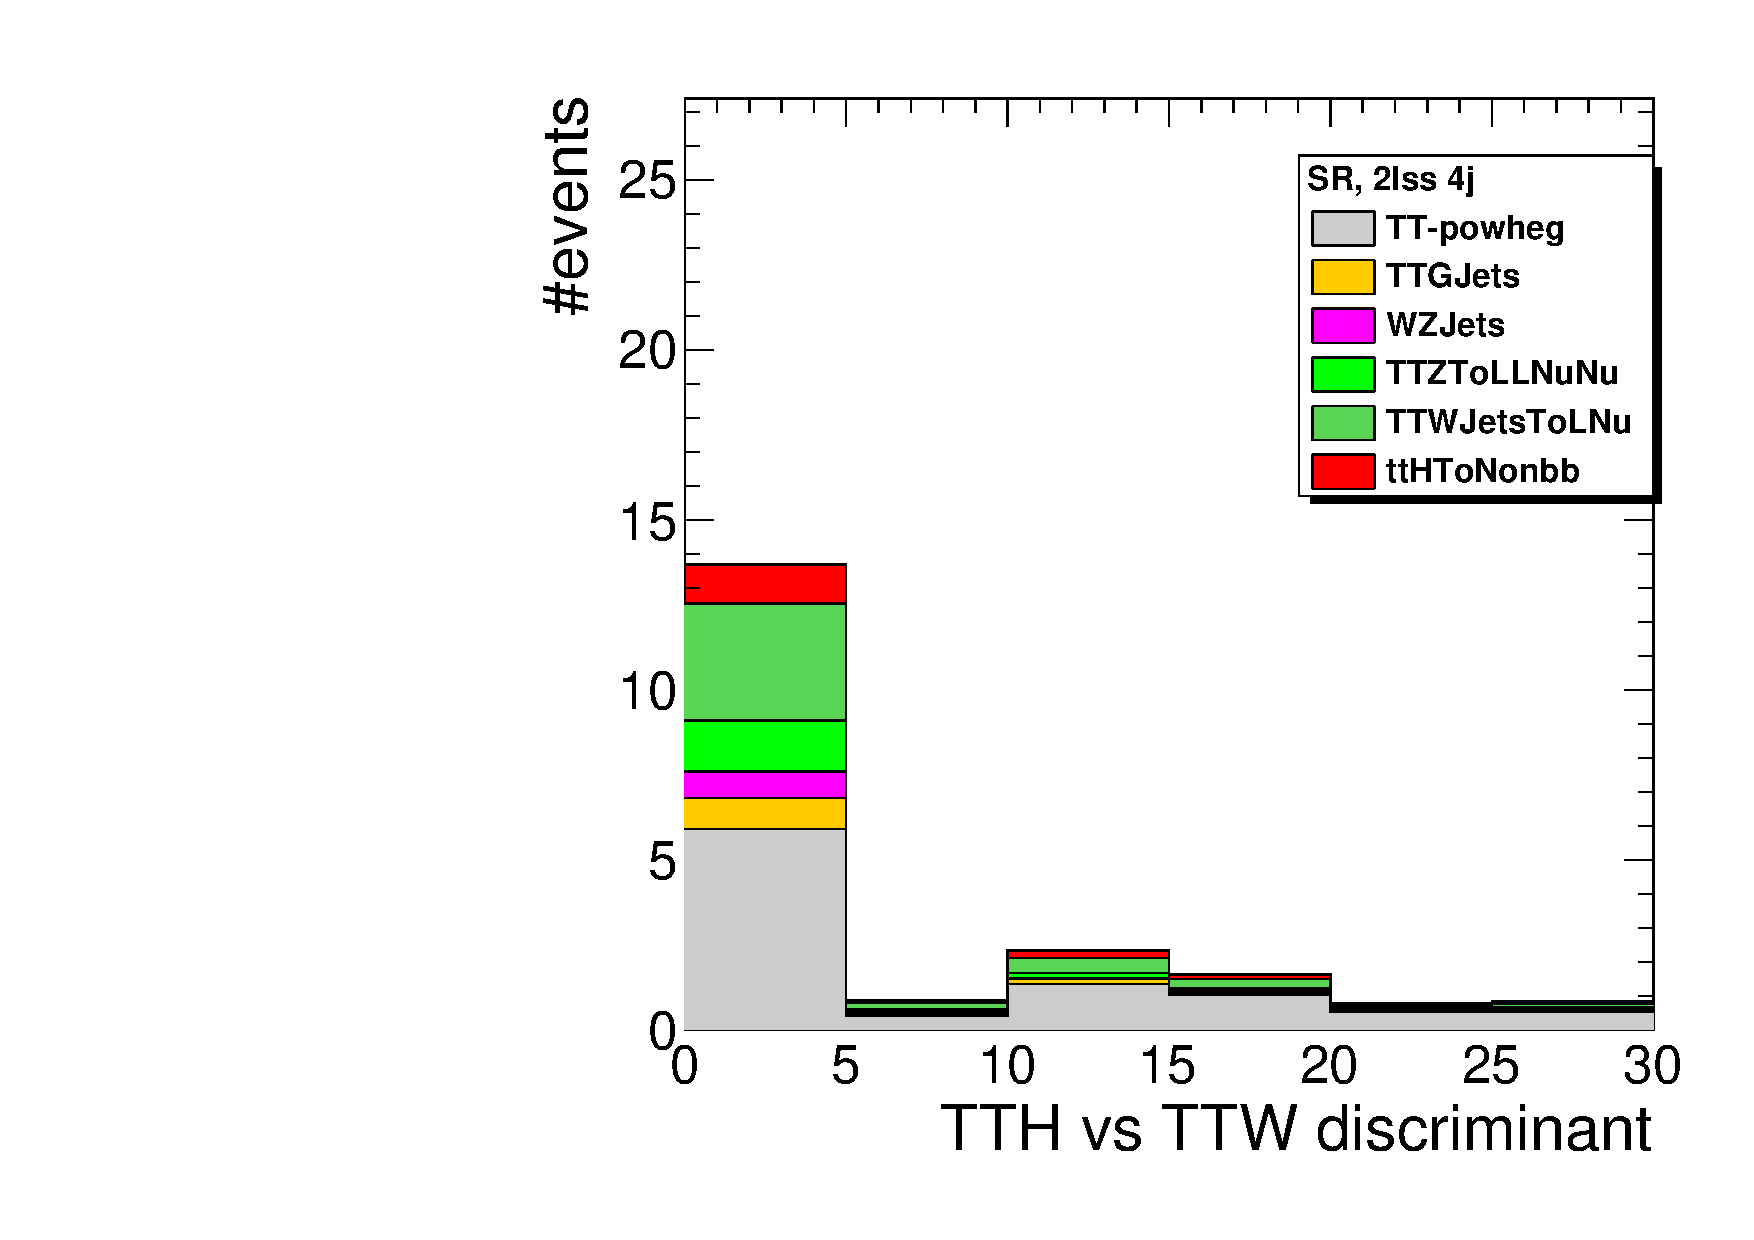
\includegraphics[width=0.4\textwidth]{plots_mem/Stack_MEMdiscriminant_2lss_SR_TTHvsTTVfull_miss2j.pdf}
   \caption{Final yields of MEM discriminants in 2lss signal region for (a) 0 missing jets, (b) 1 missing jets, (c) 2 missing jets.}
  \label{mem:memyields2lss}
\end{figure}

\begin{figure}[Htb]
 \centering
   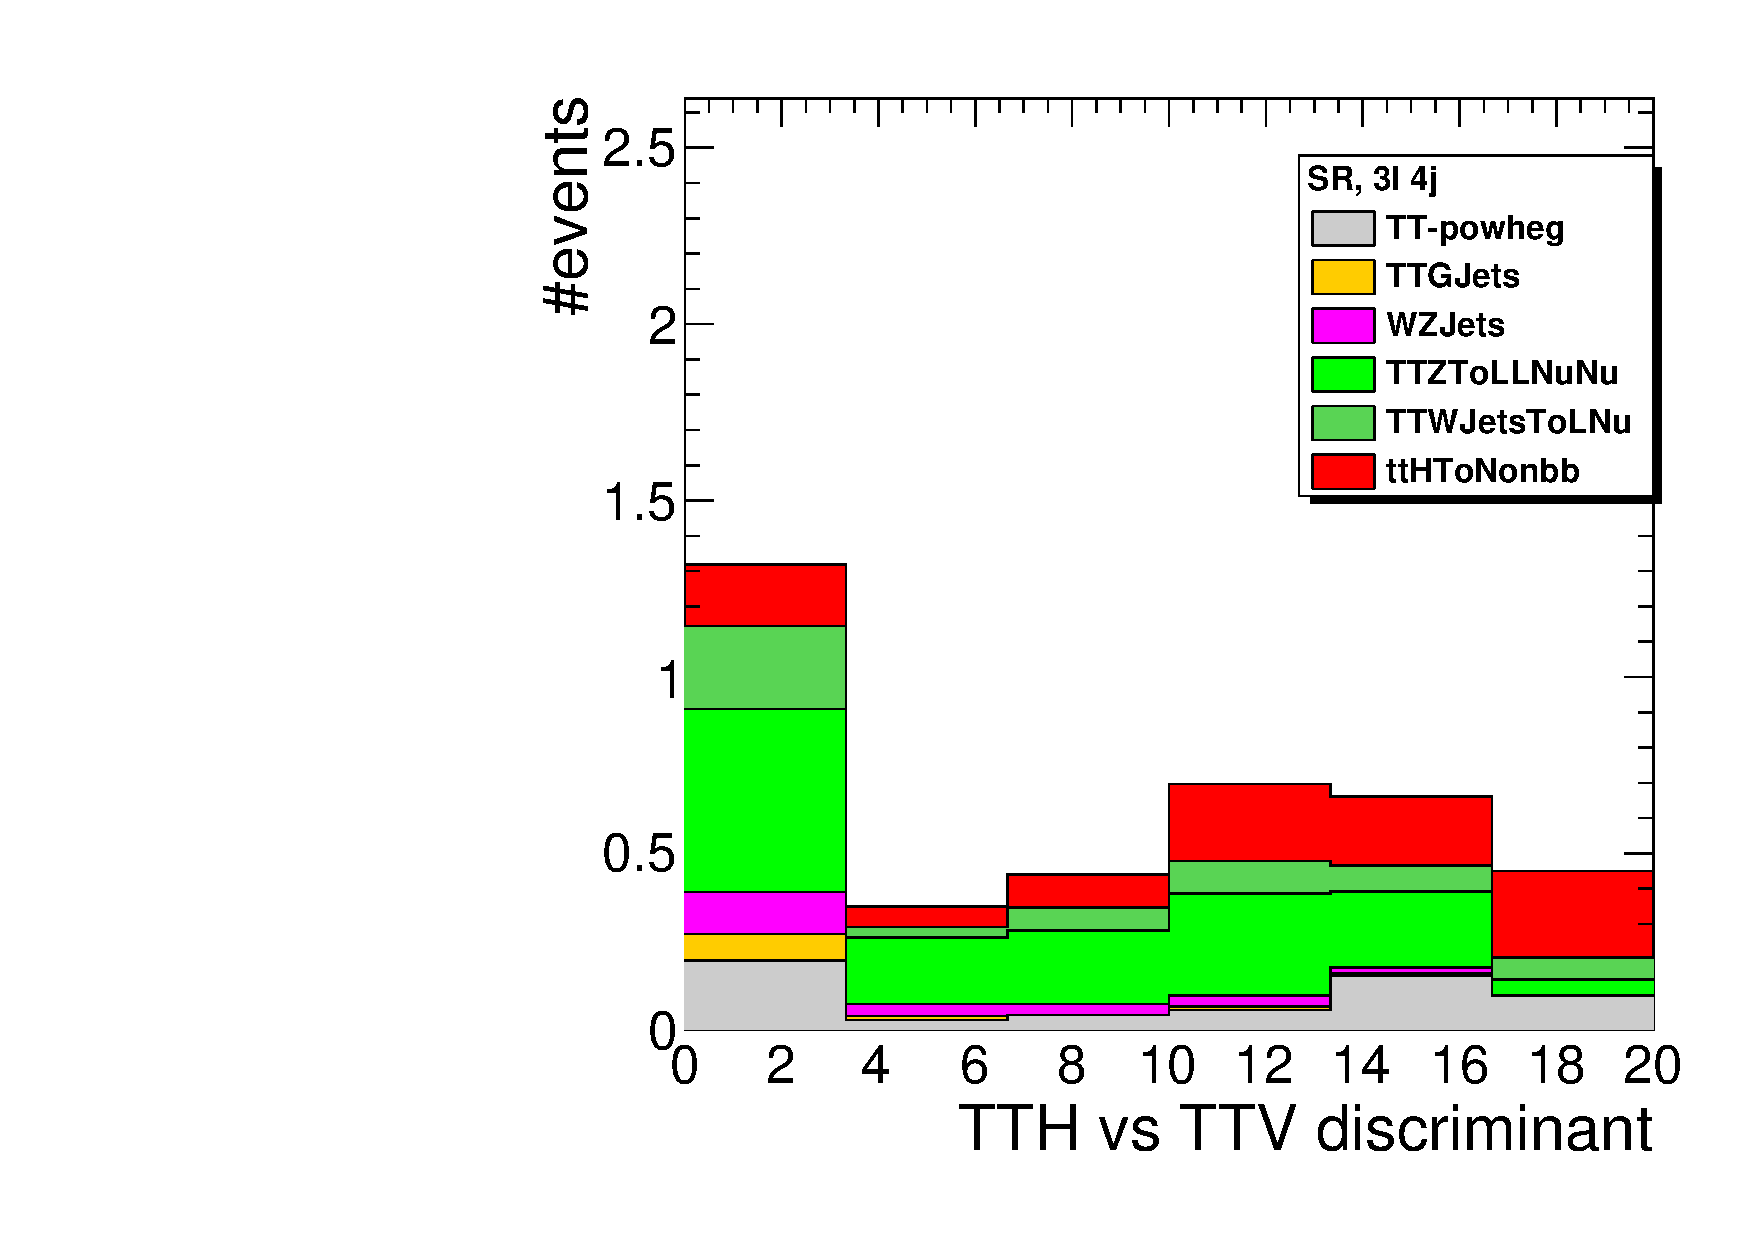
\includegraphics[width=0.4\textwidth]{plots_mem/Stack_MEMdiscriminant_3l_SR_TTHvsTTVfull_miss0j.pdf}\\
   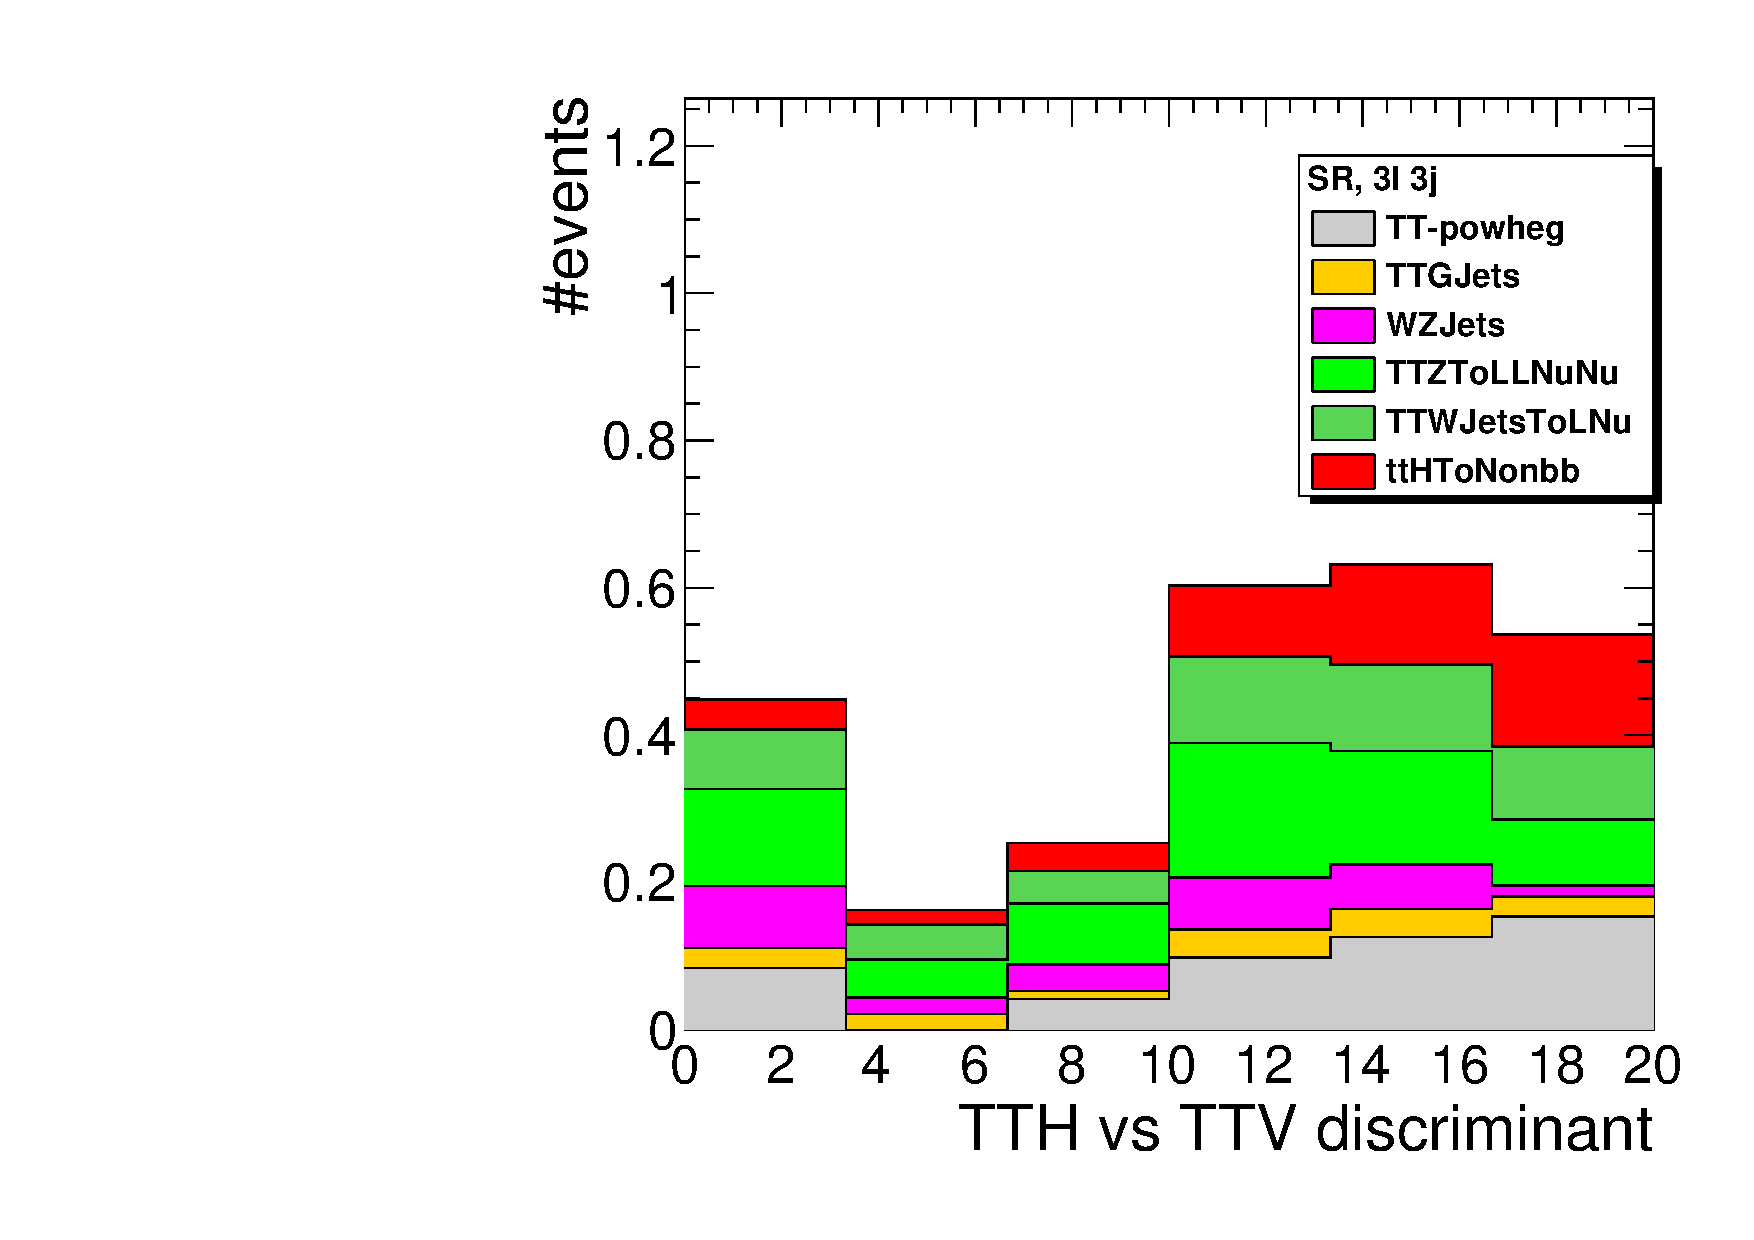
\includegraphics[width=0.4\textwidth]{plots_mem/Stack_MEMdiscriminant_3l_SR_TTHvsTTVfull_miss1j.pdf}
   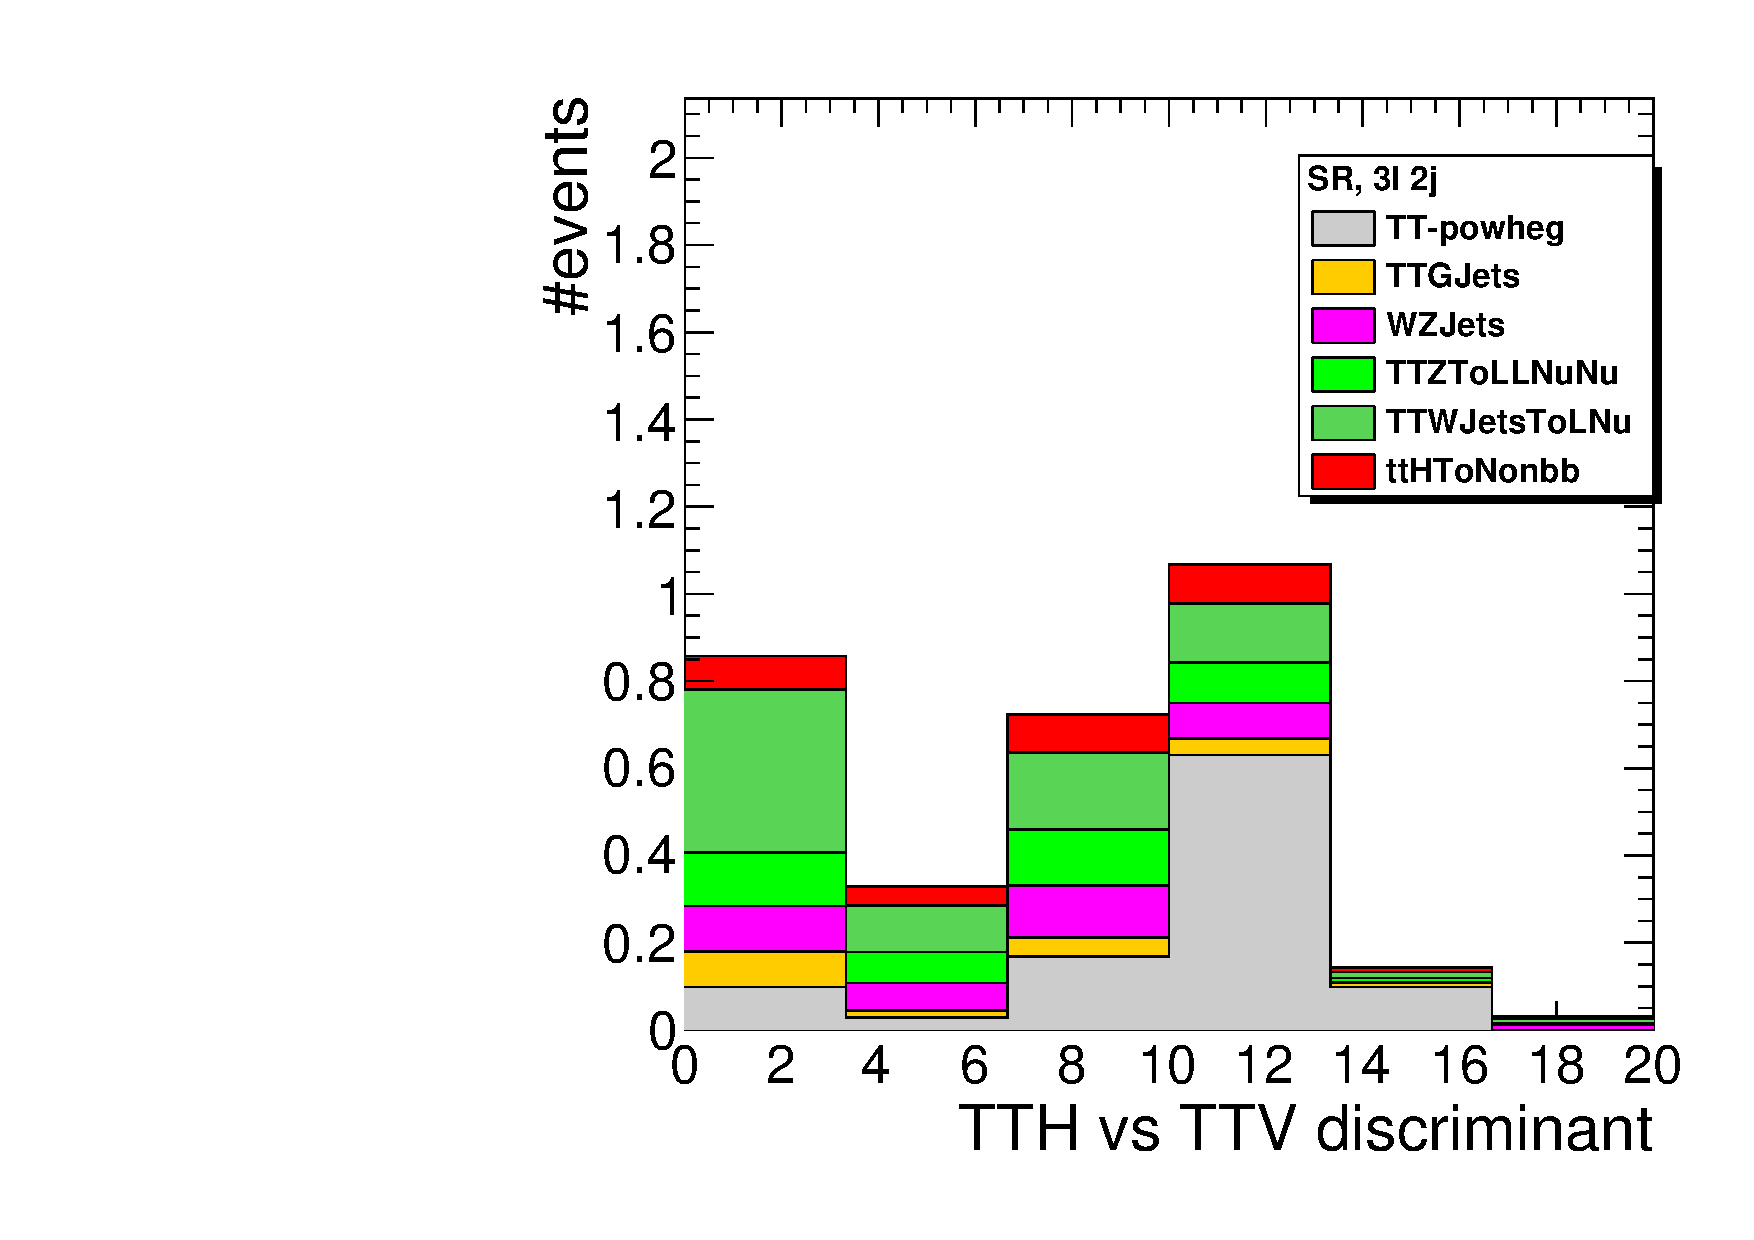
\includegraphics[width=0.4\textwidth]{plots_mem/Stack_MEMdiscriminant_3l_SR_TTHvsTTVfull_miss2j.pdf}
  \caption{Final yields of MEM discriminants in 3l signal region for (a) 0 missing jets, (b) 1 missing jets, (c) 2 missing jets.}
  \label{mem:memyields3l}
\end{figure}


\subsubsection*{Comparison with TTV BDT}

The performance of MEM discriminants is compared on fig.~\ref{mem:comparisonBDT2lss} for 2lss categories and fig.~\ref{mem:comparisonBDT3l} for 3l categories. Performance is in any case comparable, slightly lower in 2lss categories, and equivalent or slighlty better in 3l categories. The performance is better for categories where all the jets are reconstructed. There is almost no discrimination when 2 jets are missing, which is also the case for the TTV BDT.

\begin{figure}[Htb]
 \centering
%   \includegraphics[width=0.4\textwidth]{plots_mem/Moriond2017/TTV/CompareBDTvsMEM_2l_merged.pdf}\\
   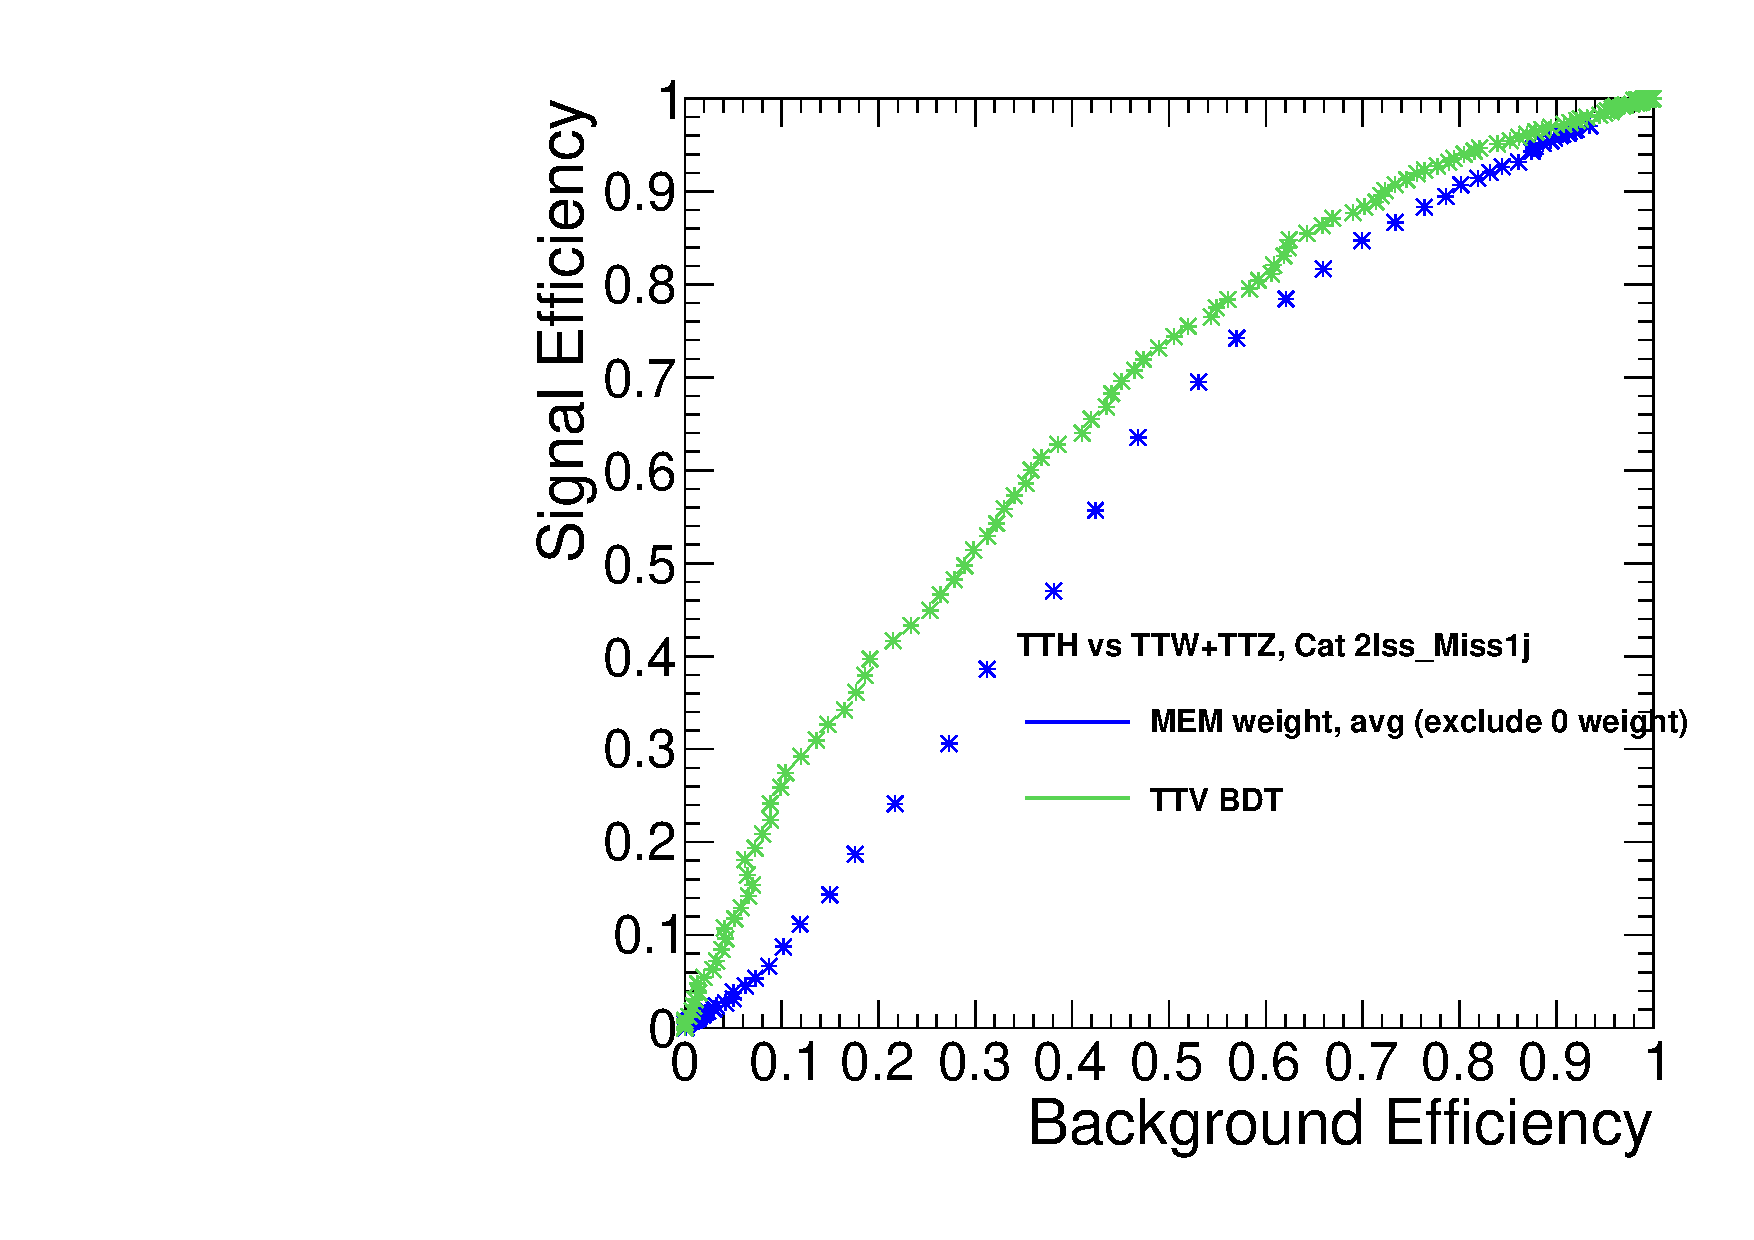
\includegraphics[width=0.4\textwidth]{plots_mem/EffSvsRejB_TTHvsTTVfull_catJets2lss_Miss1j_BDT.pdf}
%   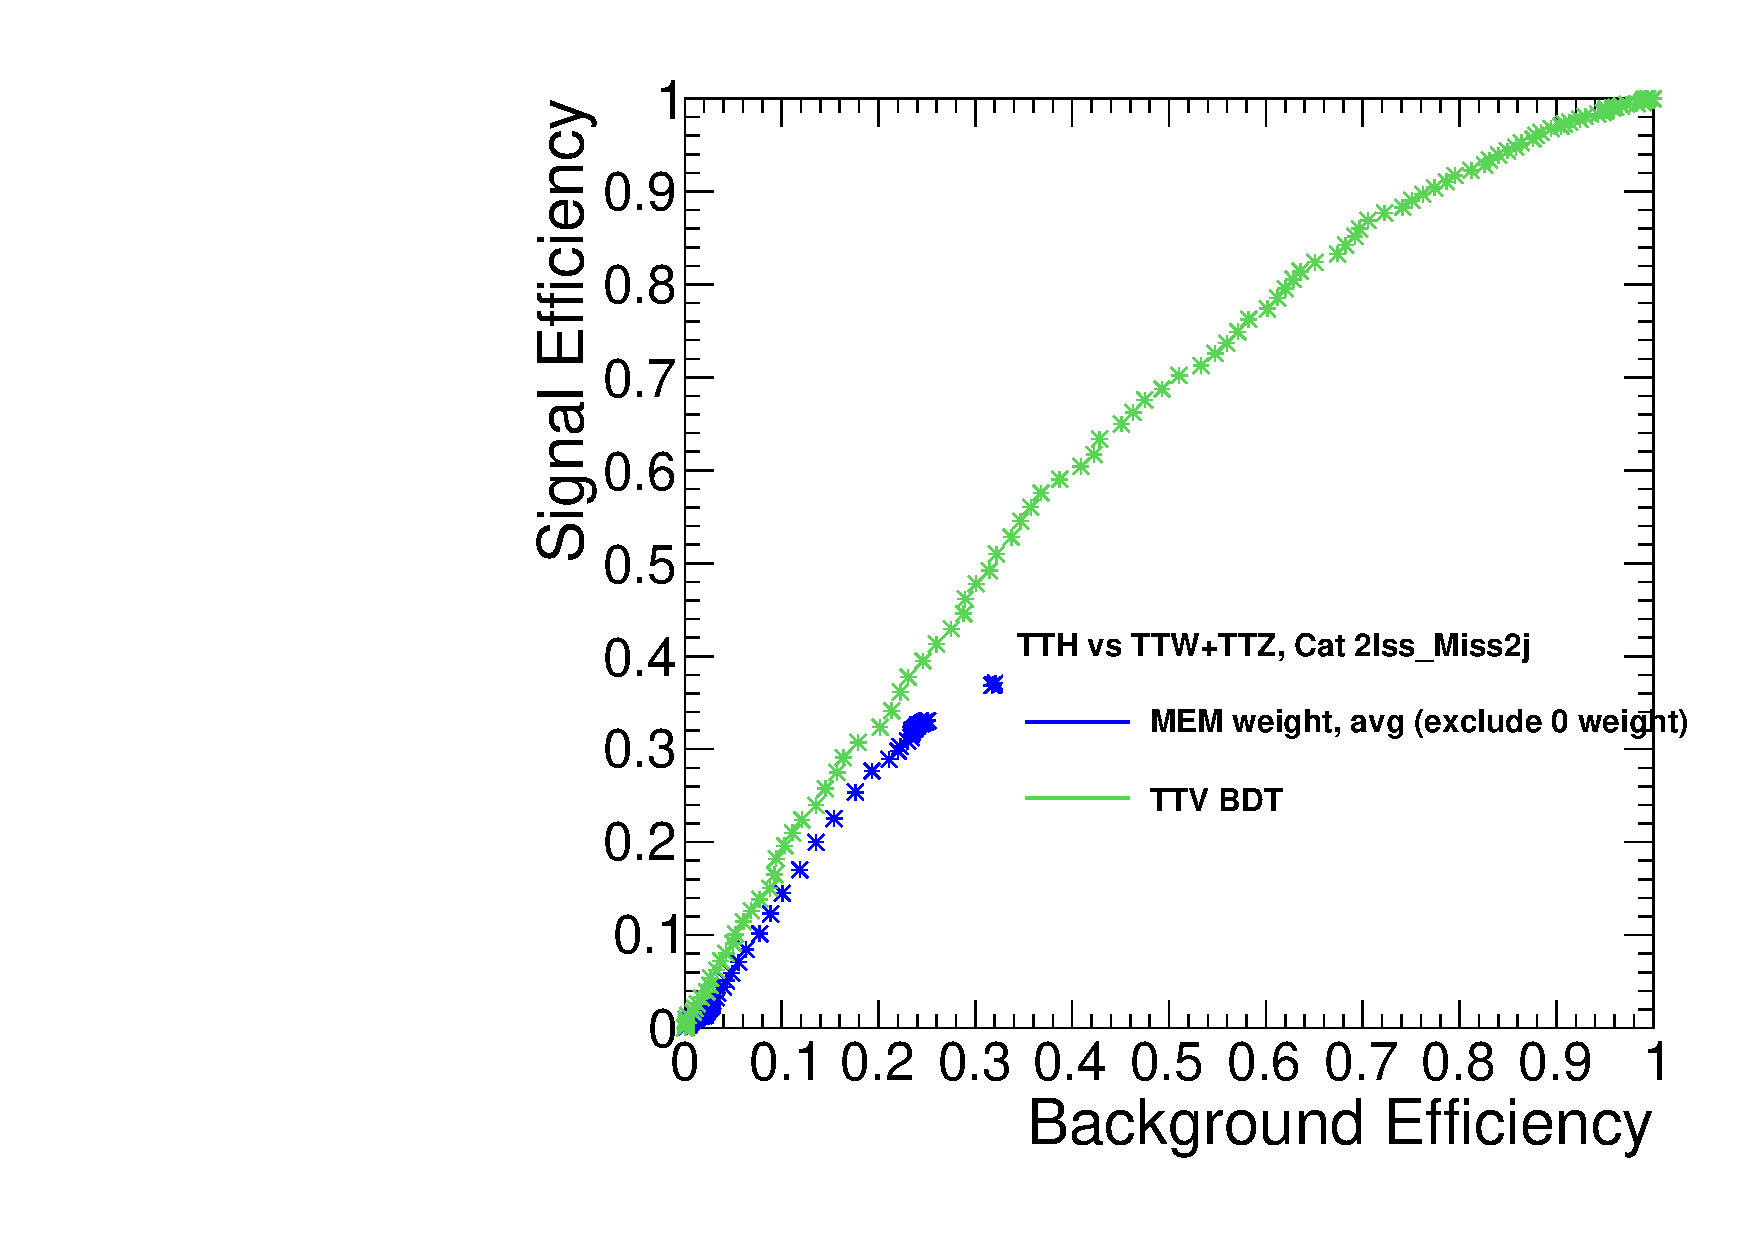
\includegraphics[width=0.4\textwidth]{plots_mem/EffSvsRejB_TTHvsTTVfull_catJets2lss_Miss2j_BDT.pdf}
   \caption{ \textcolor{red}{Not updated yet} Comparison of MEM discriminants in 2lss signal region (merged).}
% for (a) 0 missing jets, (b) 1 missing jets, (c) 2 missing jets.}
  \label{mem:comparisonBDT2lss}
\end{figure}

\begin{figure}[Htb]
 \centering
%   \includegraphics[width=0.4\textwidth]{plots_mem/Moriond2017/TTV/CompareBDTvsMEM_3l_merged.pdf}\\
   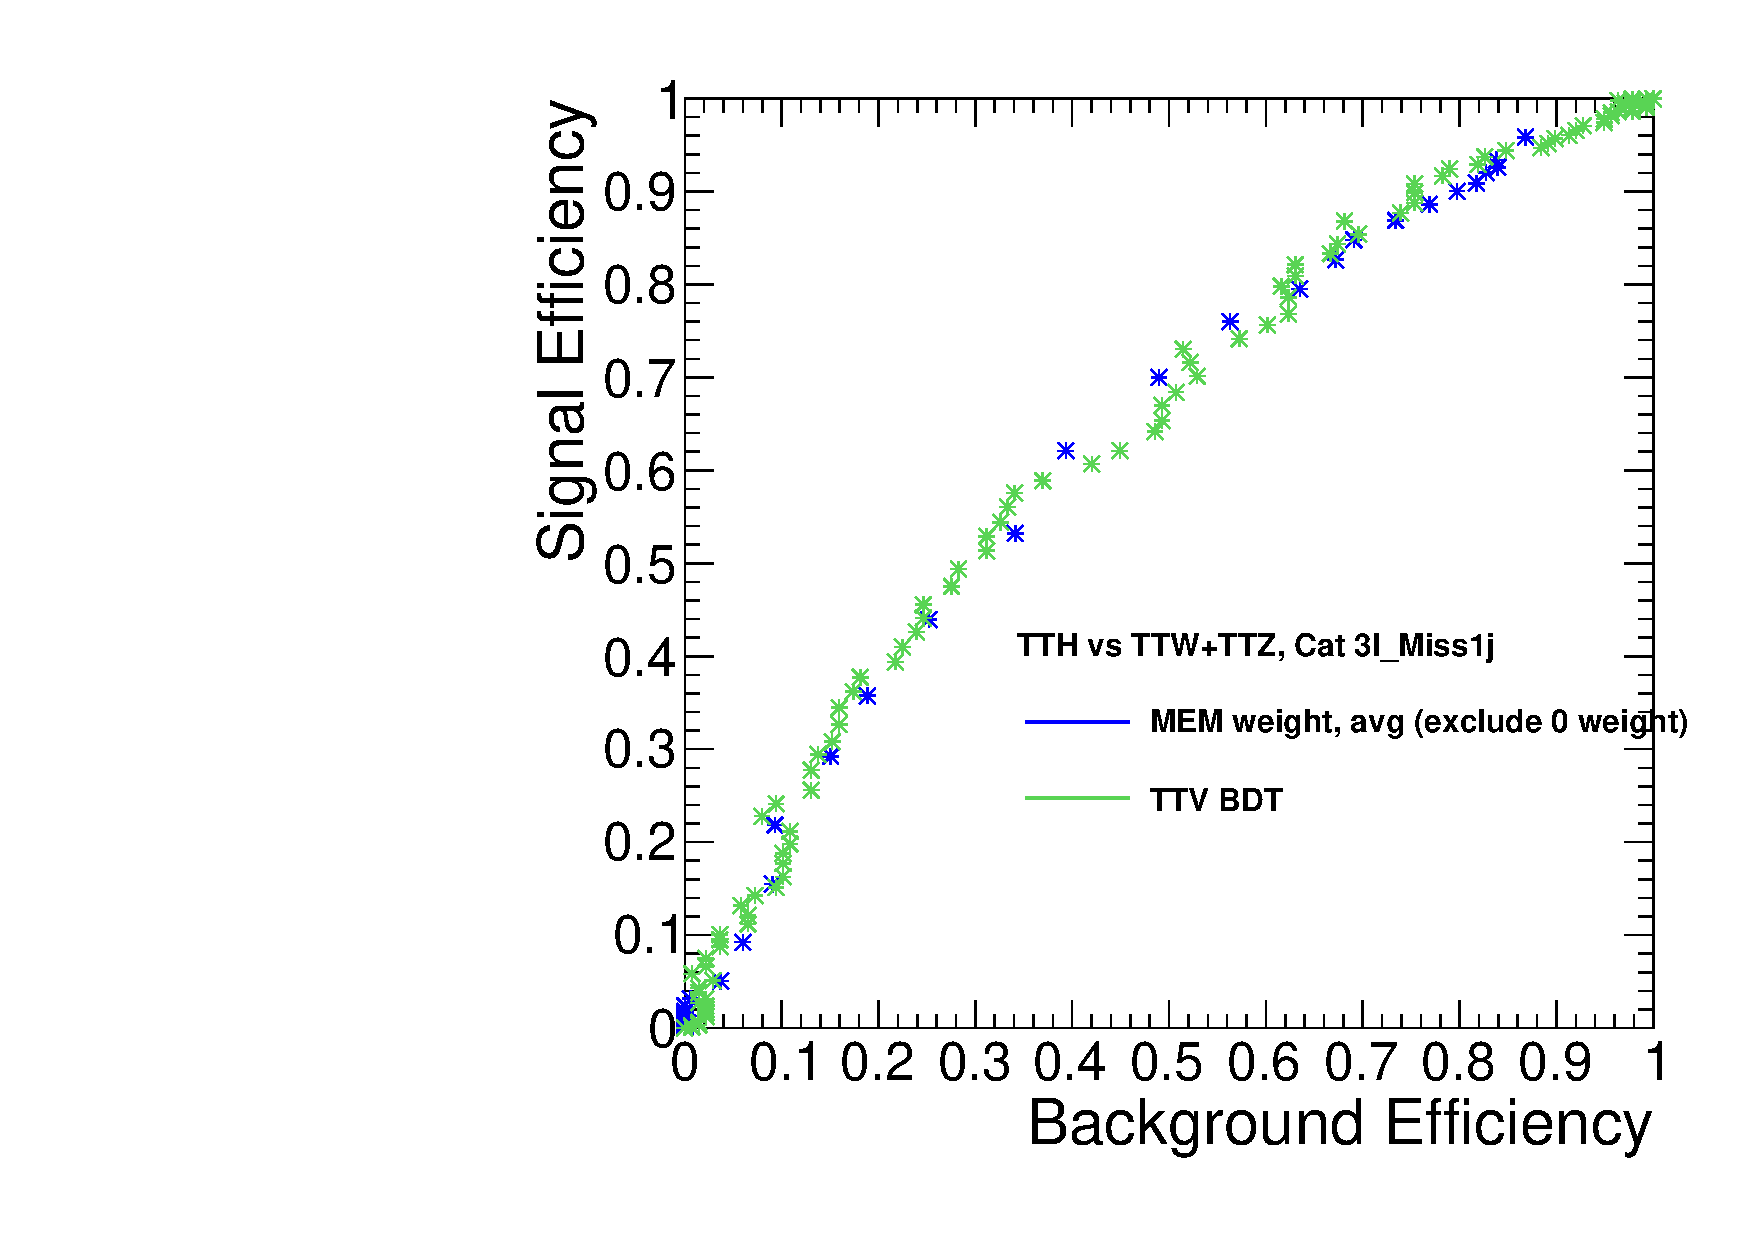
\includegraphics[width=0.4\textwidth]{plots_mem/EffSvsRejB_TTHvsTTVfull_catJets3l_Miss1j_BDT.pdf}
%   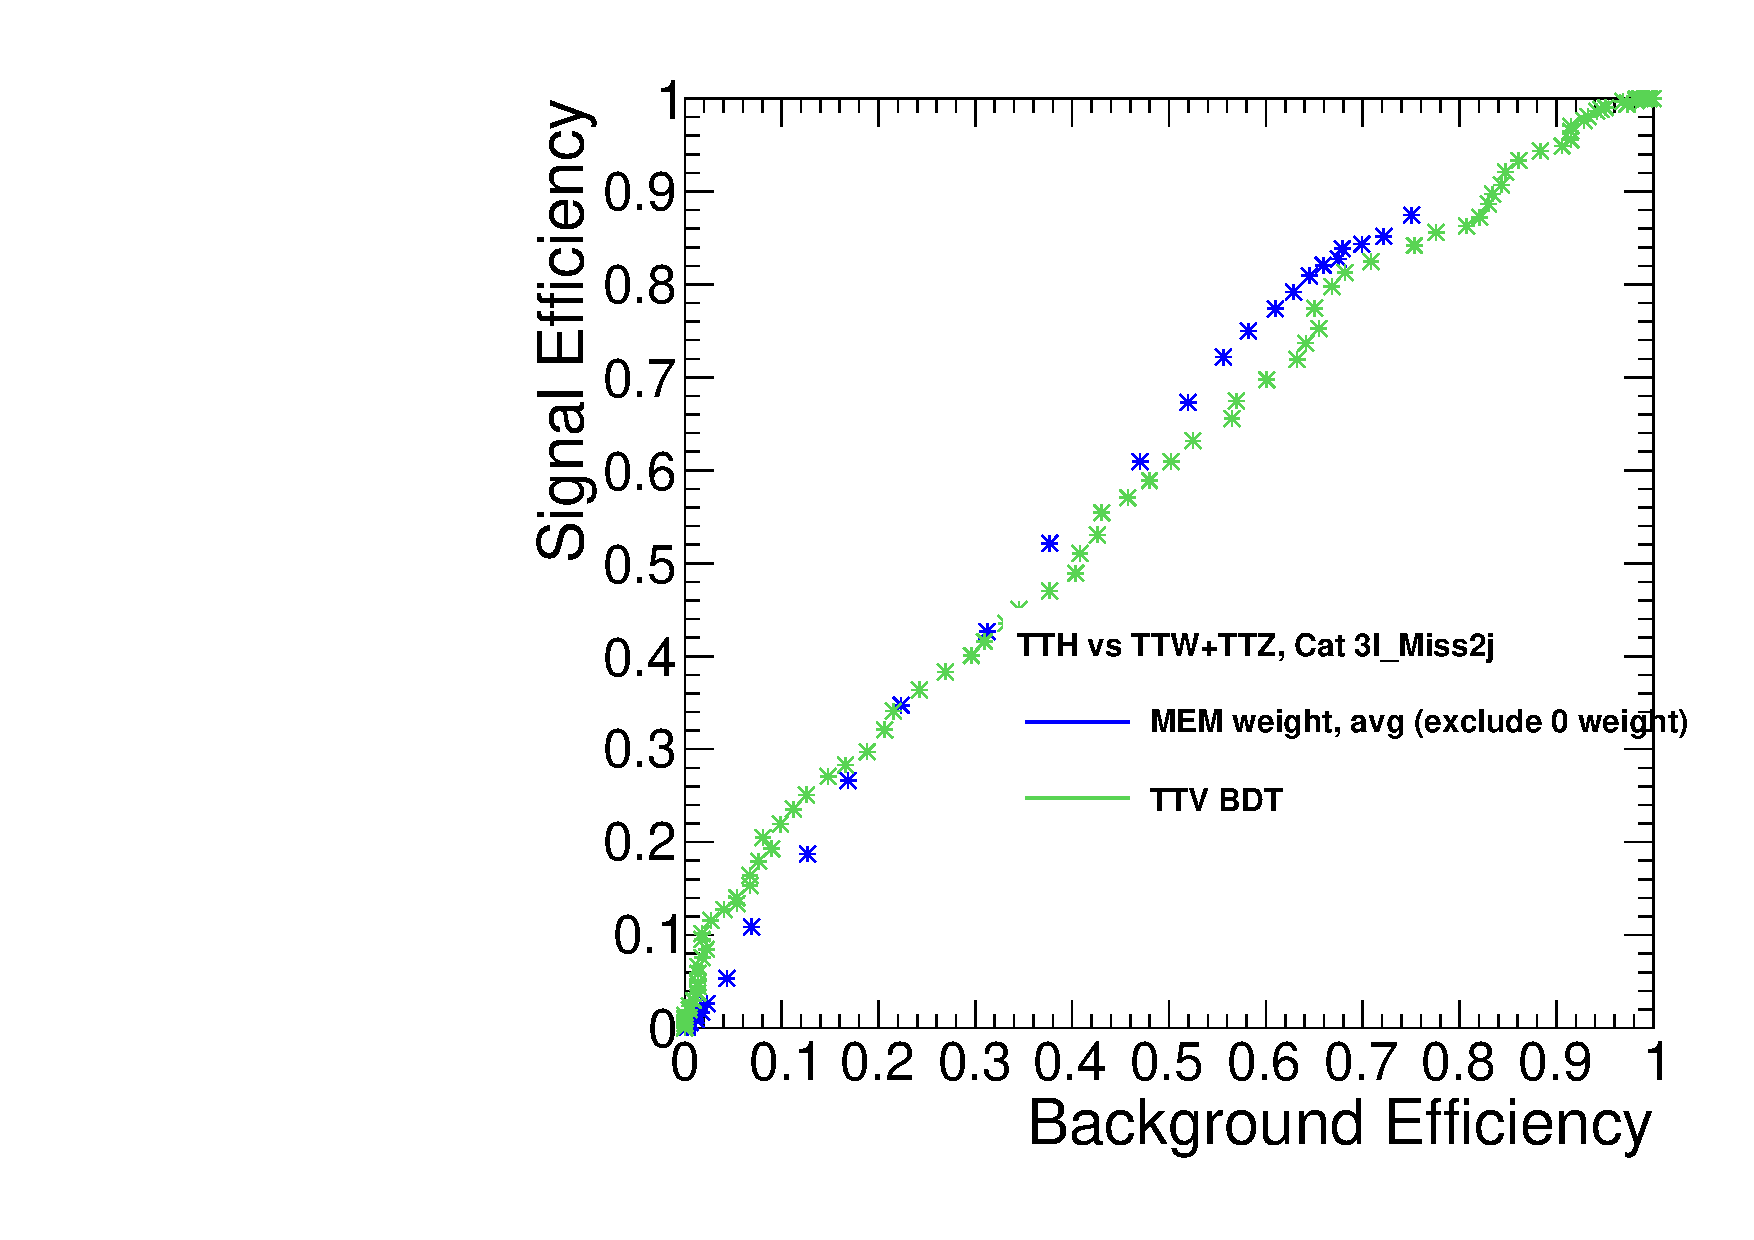
\includegraphics[width=0.4\textwidth]{plots_mem/EffSvsRejB_TTHvsTTVfull_catJets3l_Miss2j_BDT.pdf}
  \caption{ \textcolor{red}{Not updated yet} Comparison of MEM discriminants in 3l signal region (merged).}
% for (a) 0 missing jets, (b) 1 missing jets, (c) 2 missing jets.}
  \label{mem:comparisonBDT3l}
\end{figure}


\subsubsection*{MEM as input variable to the TTV BDT}\label{sec:meminput}

Given that the performances of TTV BDT and MEM discriminants are similar, it makes sense to train BDT including the MEM.
We train new BDT's using Madgraph $t\bar{t}W$ and $t\bar{t}Z$ large samples with same setup used for training BDT TTV, but including MEM weights. Three trainings are performed:
\begin{itemize}
\item 2lss category: TTV BDT inputs + $log(w_{TTH})$ + $log(w_{TTW})$ + catJets, where catJets is the jet category (0/1/2-missing jets)
\item 3l/4l categories with a SFOS lepton pair: TTV BDT inputs + $log(w_{TTH})$ + $log(w_{TTW})$ + $log(w_{TTZ})$ + catJets
\item 3l categories without SFOS lepton pair: TTV BDT inputs + $log(w_{TTH})$ + $log(w_{TTW})$ + catJets
\end{itemize}
The $log(w)$ are the $log$ of average MEM weight excluding null weights. catJets variable is included to make the BDT aware of the missing jet category.

Results are shown on fig.\ref{mem:BDTMEMtraining2lss} for 2lss category, fig.\ref{mem:BDTMEMtraining3lnoSFOS} for 3l without SFOS lepton pair, fig.~\ref{mem:BDTMEMtraining3lSFOS} for 3l with a SFOS lepton pair, and fig.~\ref{mem:BDTMEMtraining4l} for 4l. Performance of BDT including MEM is greater than the previous training of TTV BDT for all categories, by a few \% in signal efficiency for a given background rejection in 2lss categories and up to 10-15\% in 3l and 4l categories.


\begin{figure}[Htb]
 \centering
   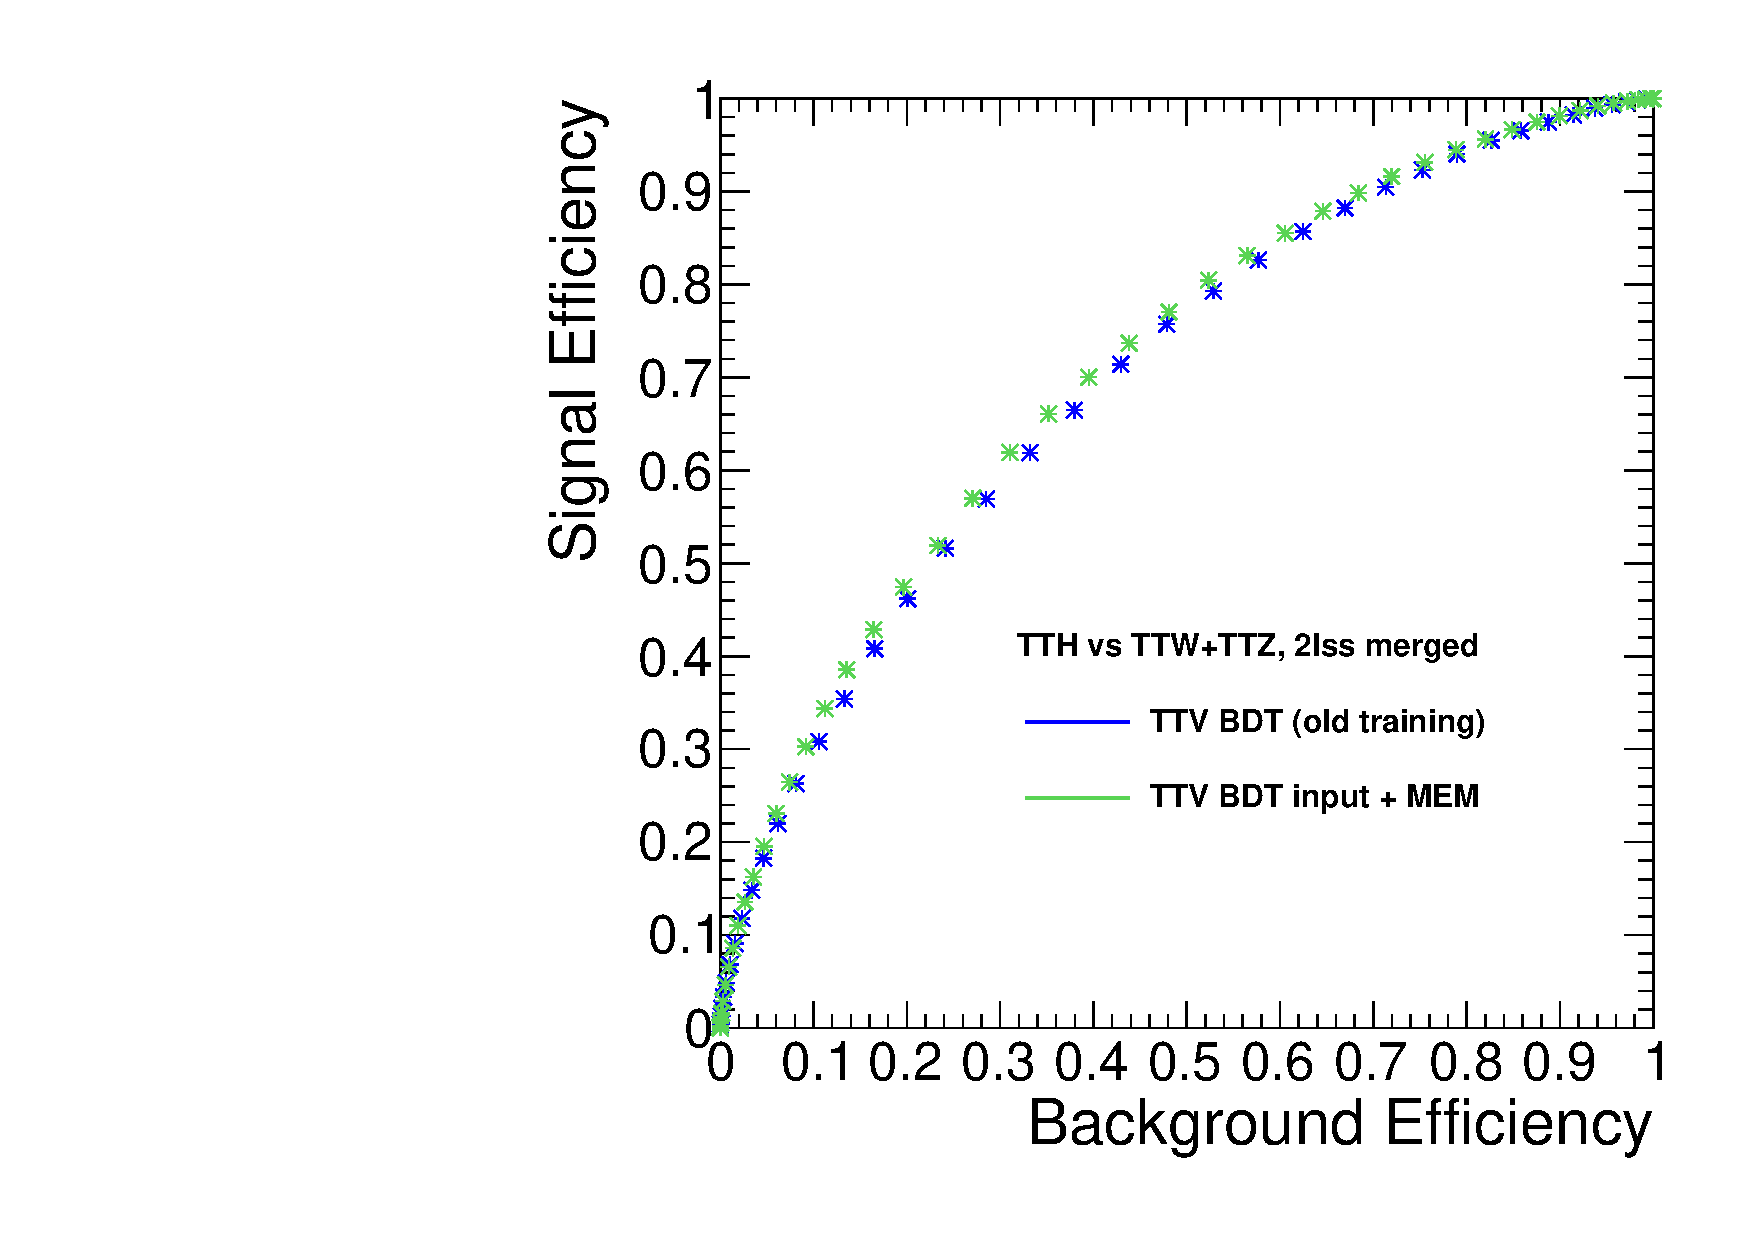
\includegraphics[width=0.4\textwidth]{plots_mem/Moriond2017/TTV/CompareBDT_2lss_merged.pdf}
   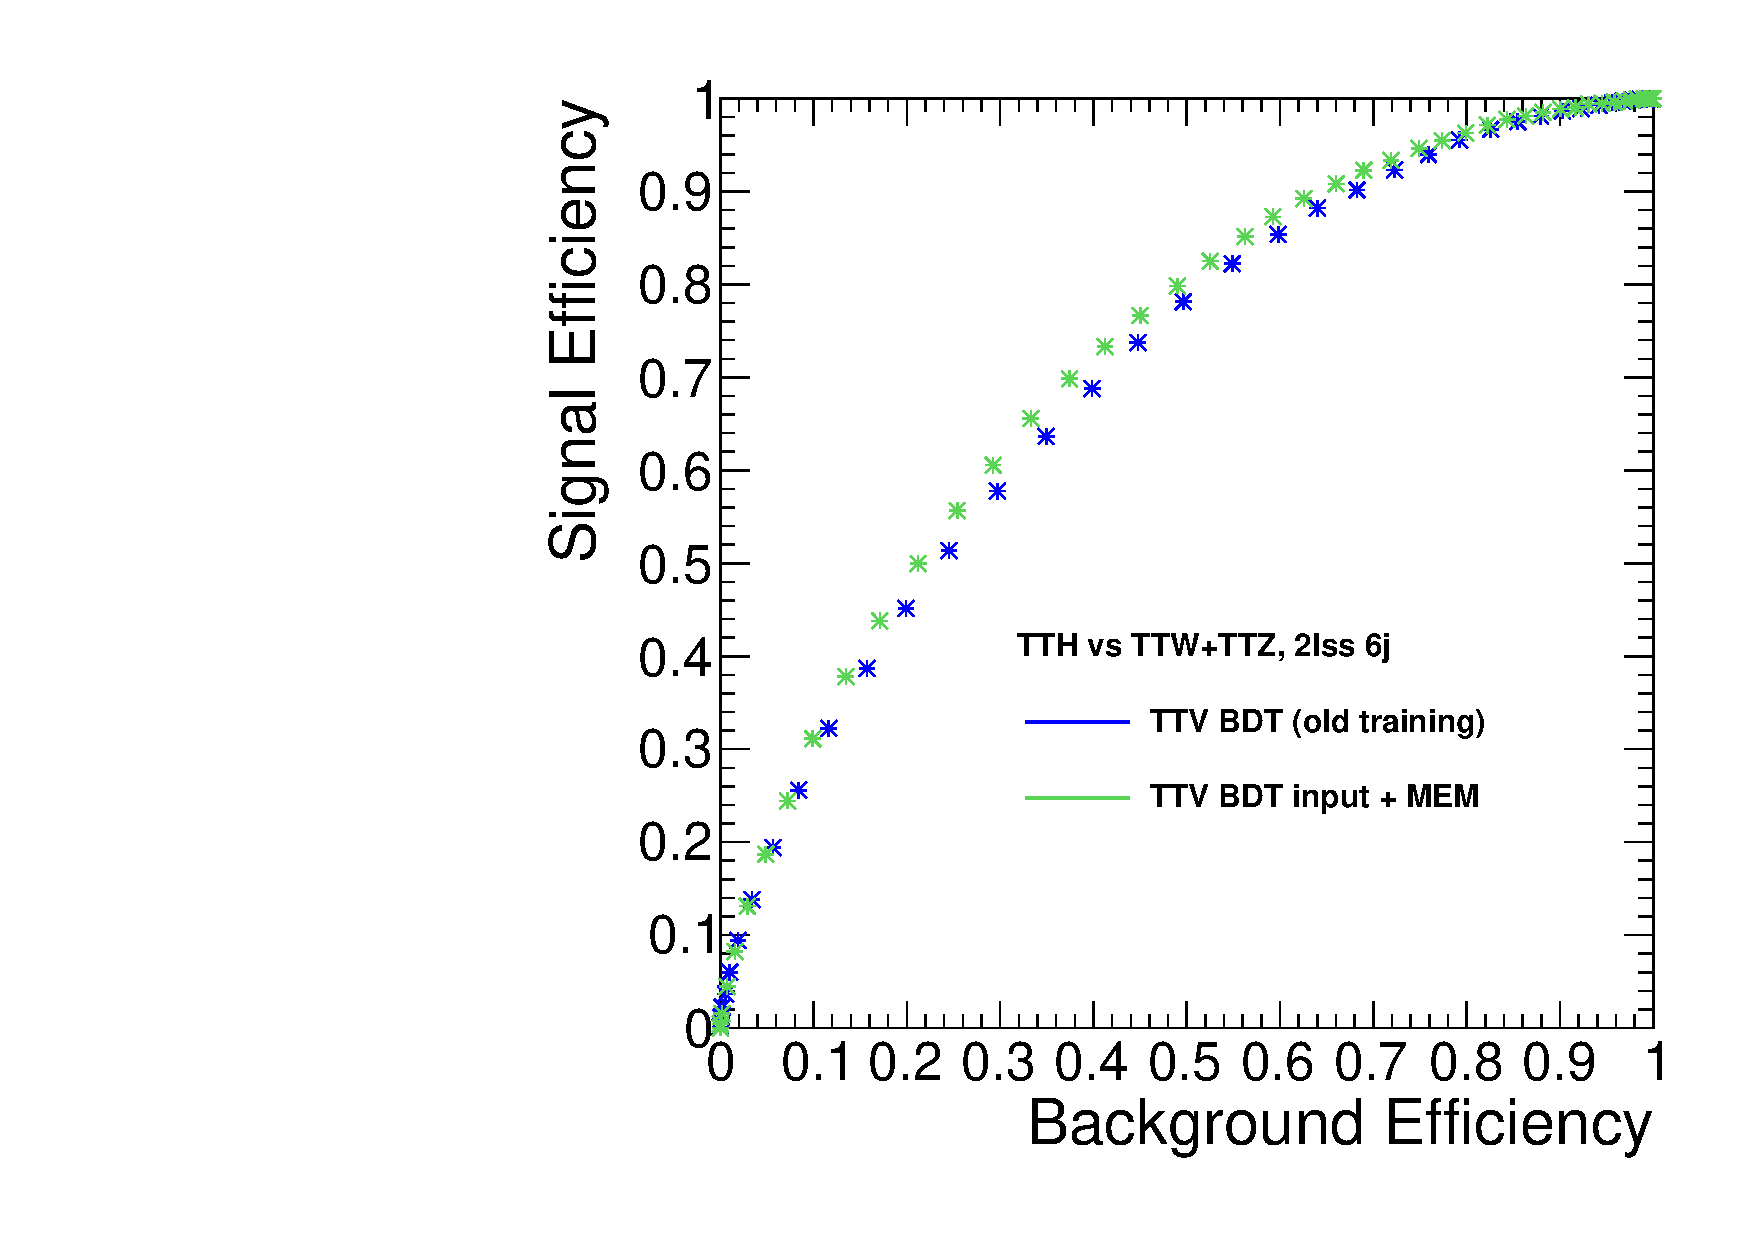
\includegraphics[width=0.4\textwidth]{plots_mem/Moriond2017/TTV/CompareBDT_2lss_6j.pdf}\\
   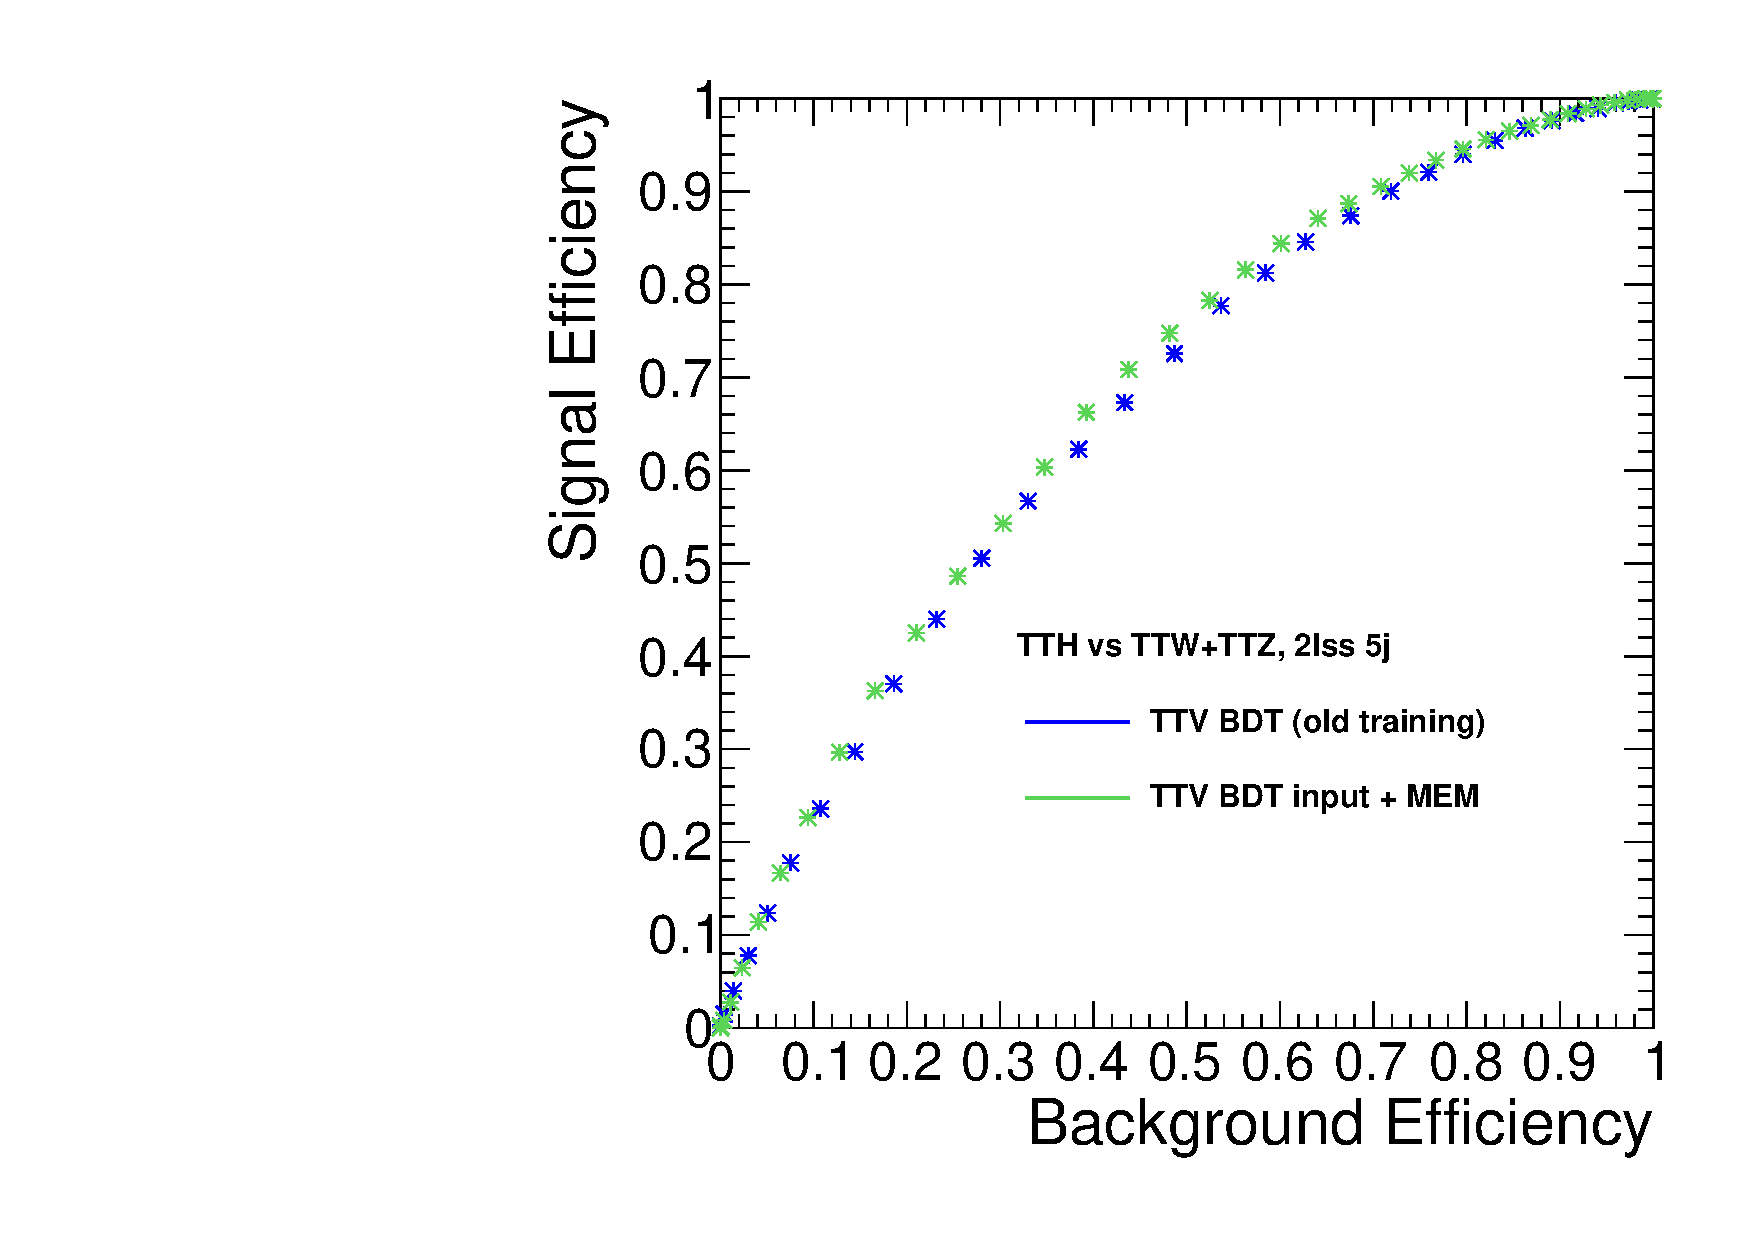
\includegraphics[width=0.4\textwidth]{plots_mem/Moriond2017/TTV/CompareBDT_2lss_5j.pdf}
   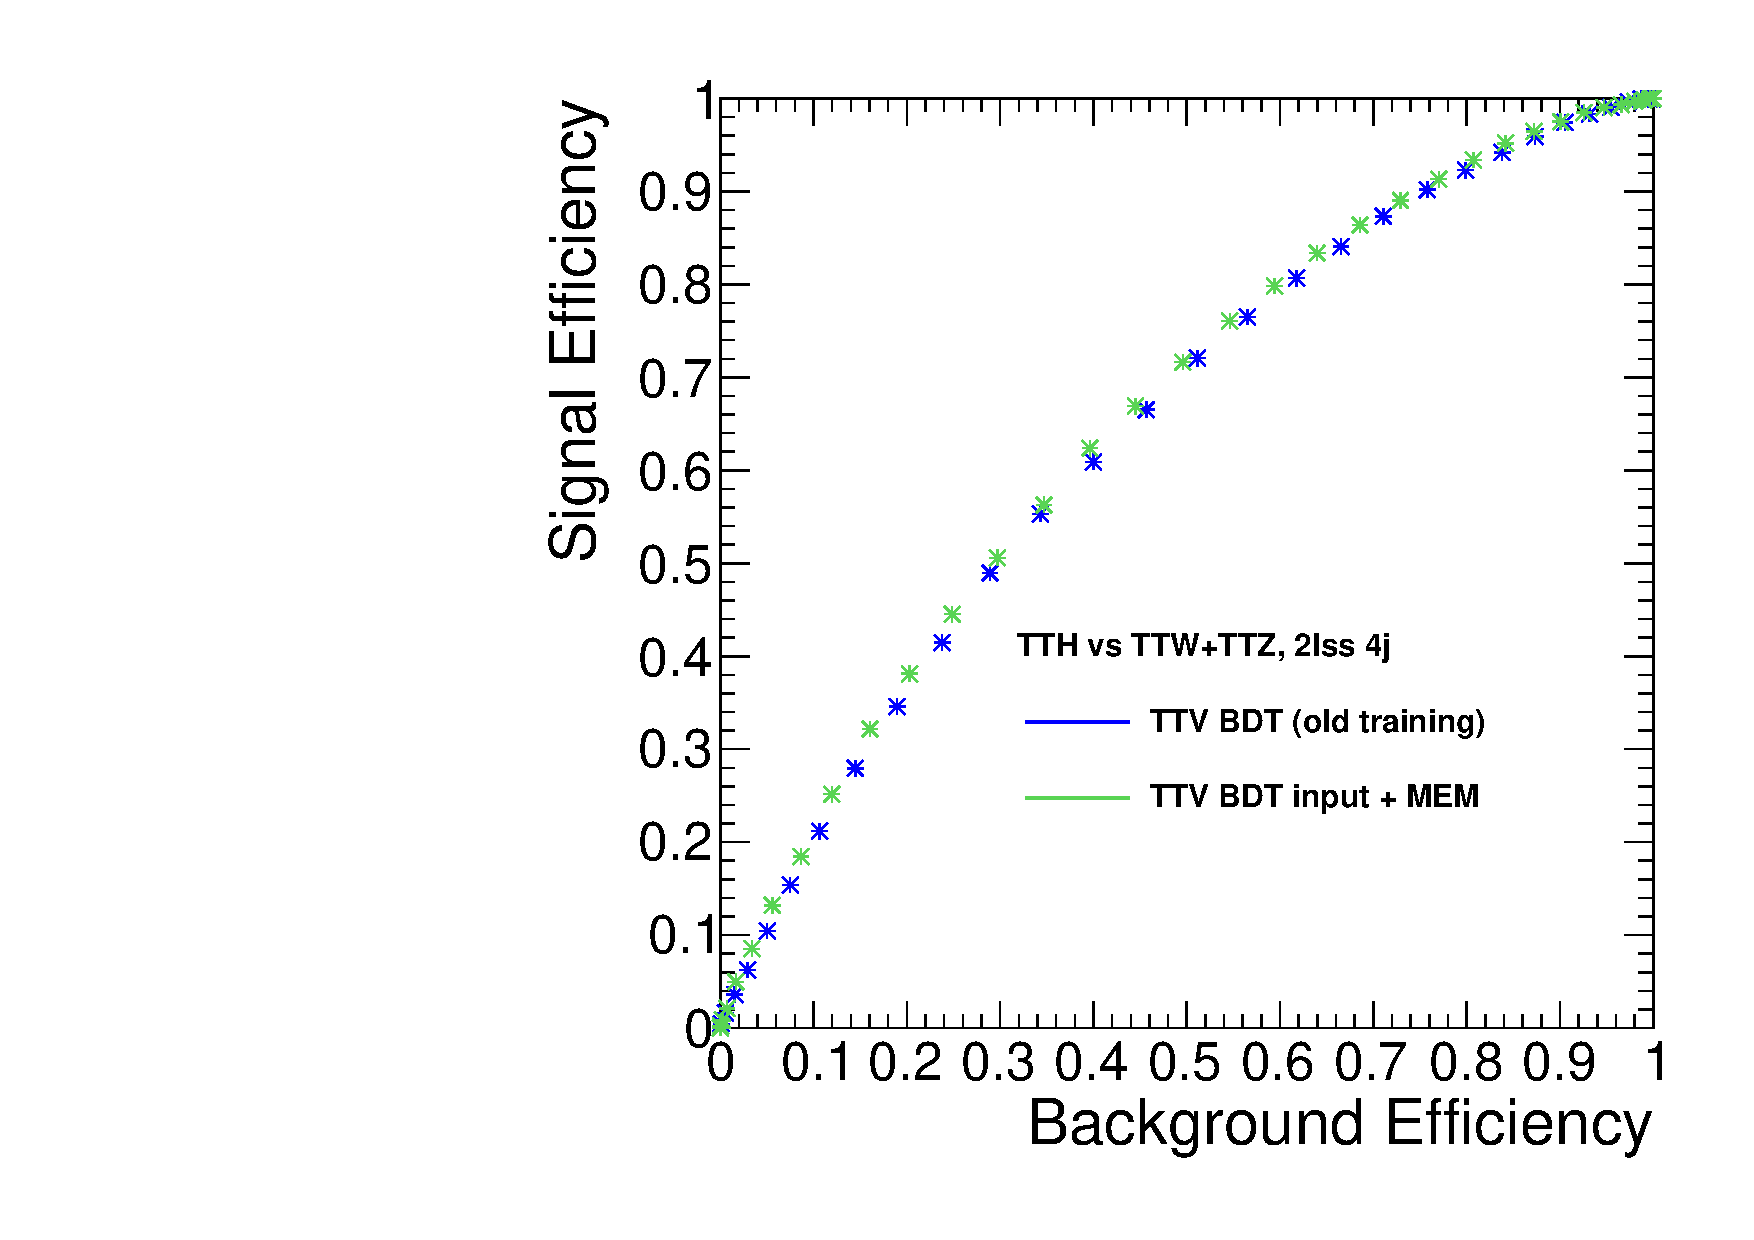
\includegraphics[width=0.4\textwidth]{plots_mem/Moriond2017/TTV/CompareBDT_2lss_4j.pdf}
   \caption{ \textcolor{green}{Updated} Comparison of TTV BDT and new BDT including MEM in 2lss signal region for (a) all events (b) 0 missing jets, (c) 1 missing jets, (d) 2 missing jets.}
  \label{mem:BDTMEMtraining2lss}
\end{figure}

\begin{figure}[Htb]
 \centering
   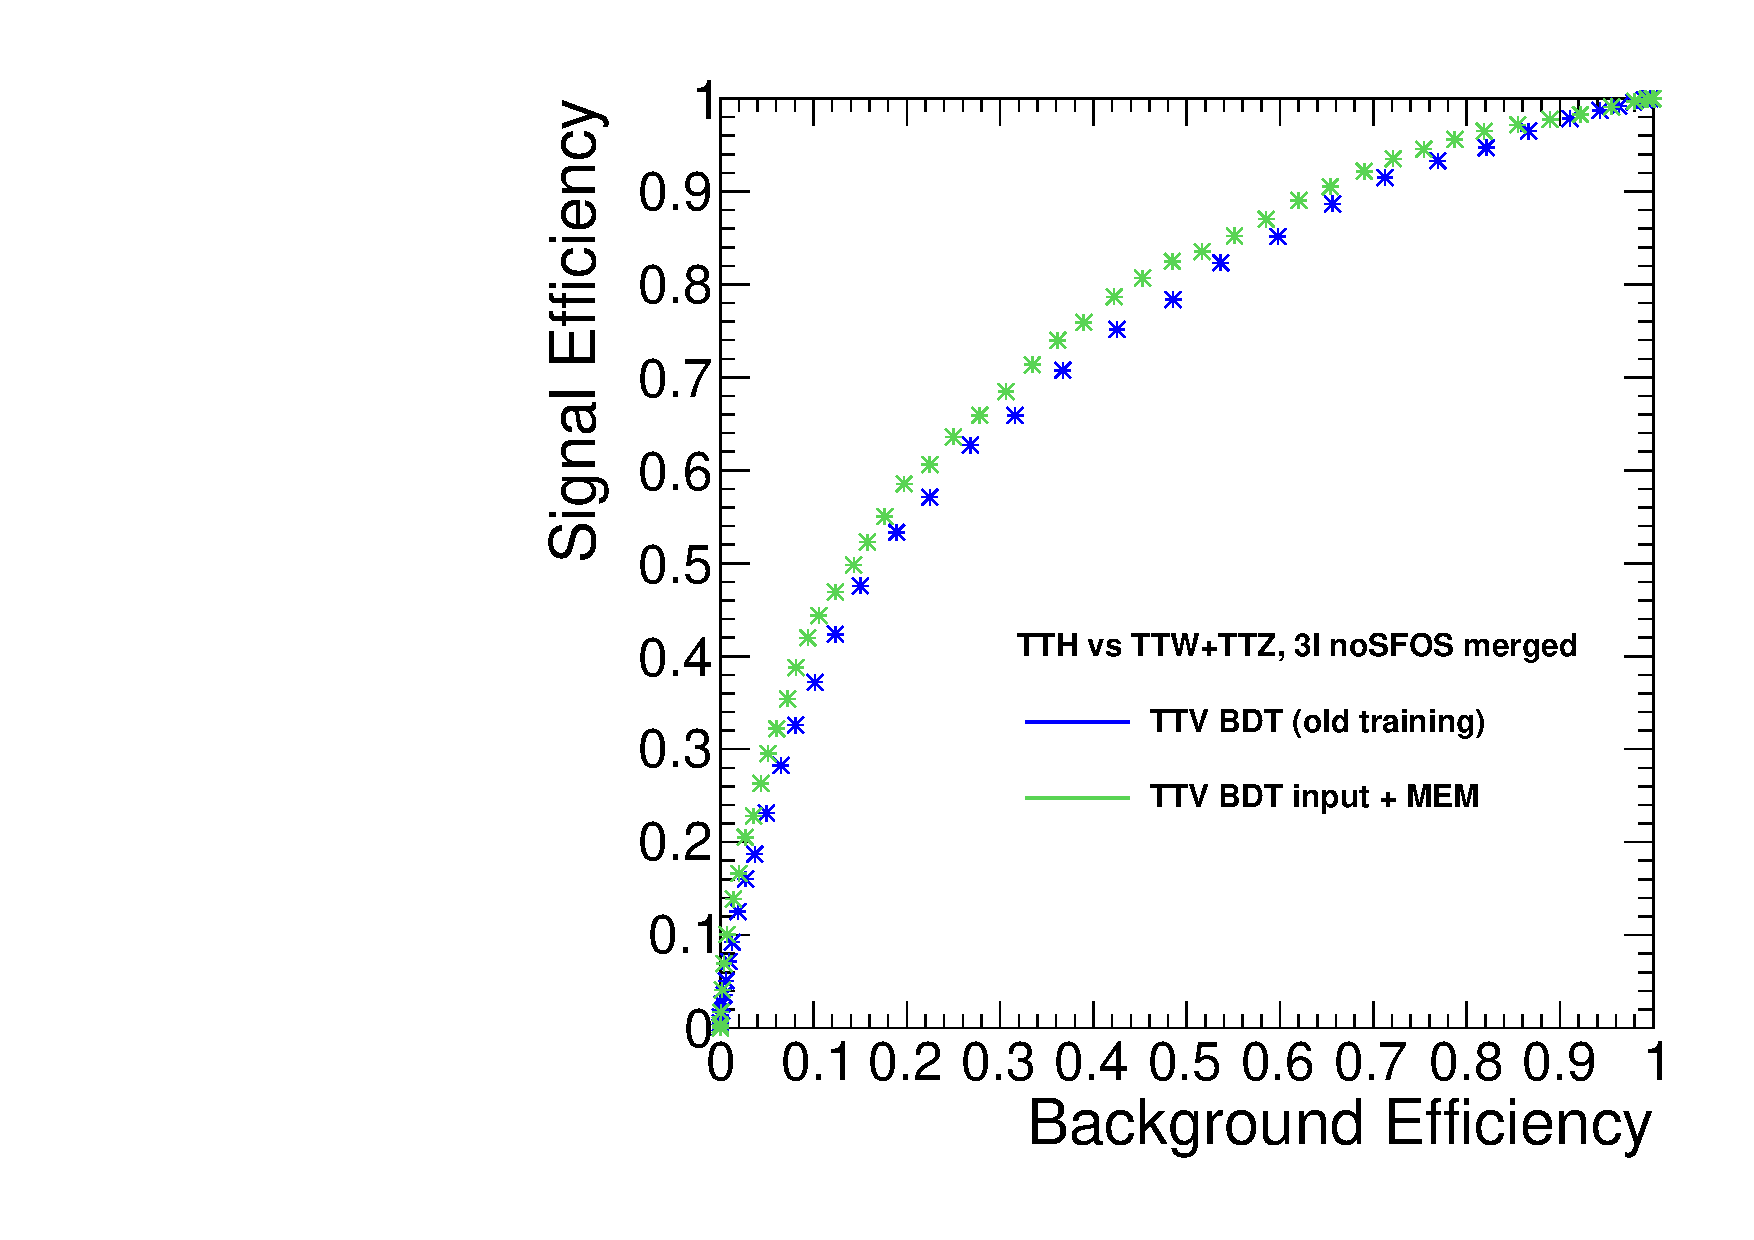
\includegraphics[width=0.4\textwidth]{plots_mem/Moriond2017/TTV/CompareBDT_3l_noSFOS_merged.pdf}
   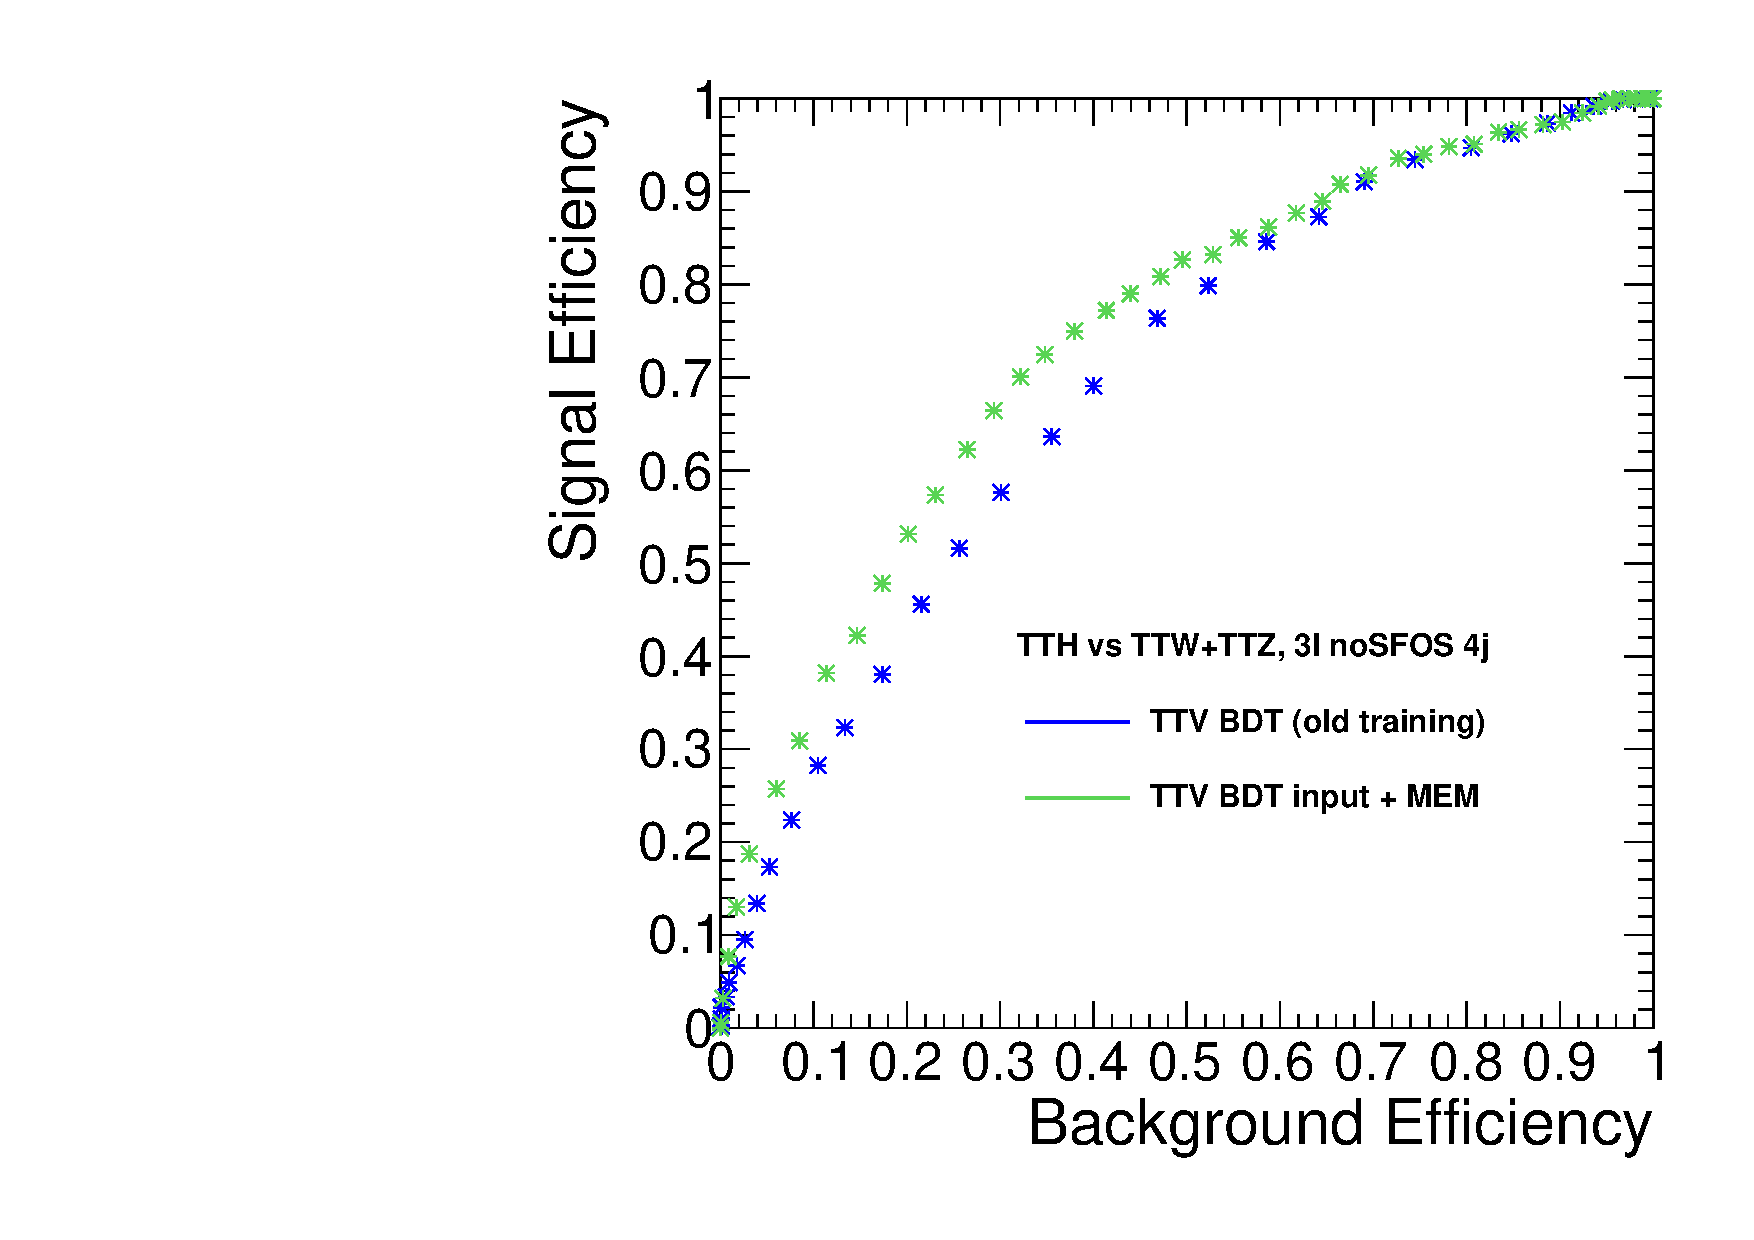
\includegraphics[width=0.4\textwidth]{plots_mem/Moriond2017/TTV/CompareBDT_3l_noSFOS_4j.pdf}\\
   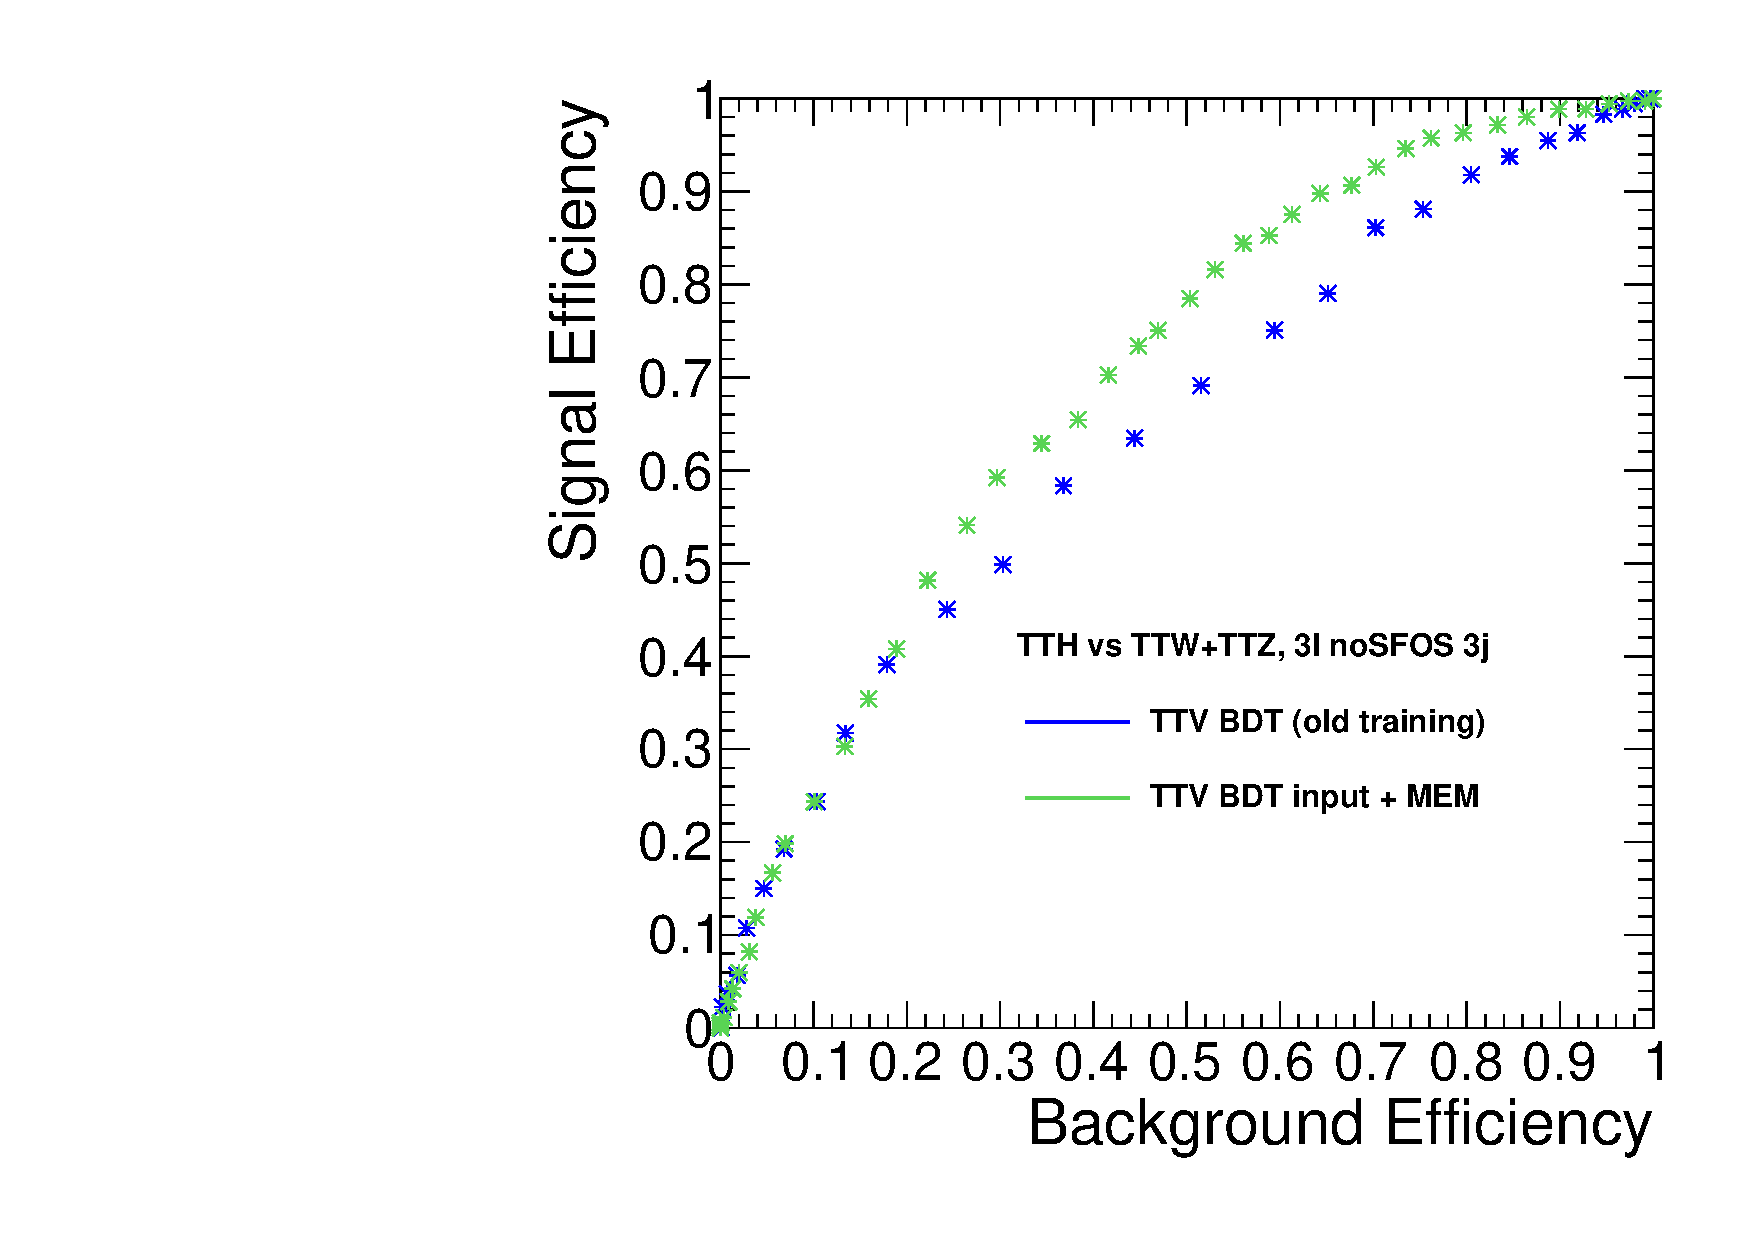
\includegraphics[width=0.4\textwidth]{plots_mem/Moriond2017/TTV/CompareBDT_3l_noSFOS_3j.pdf}
   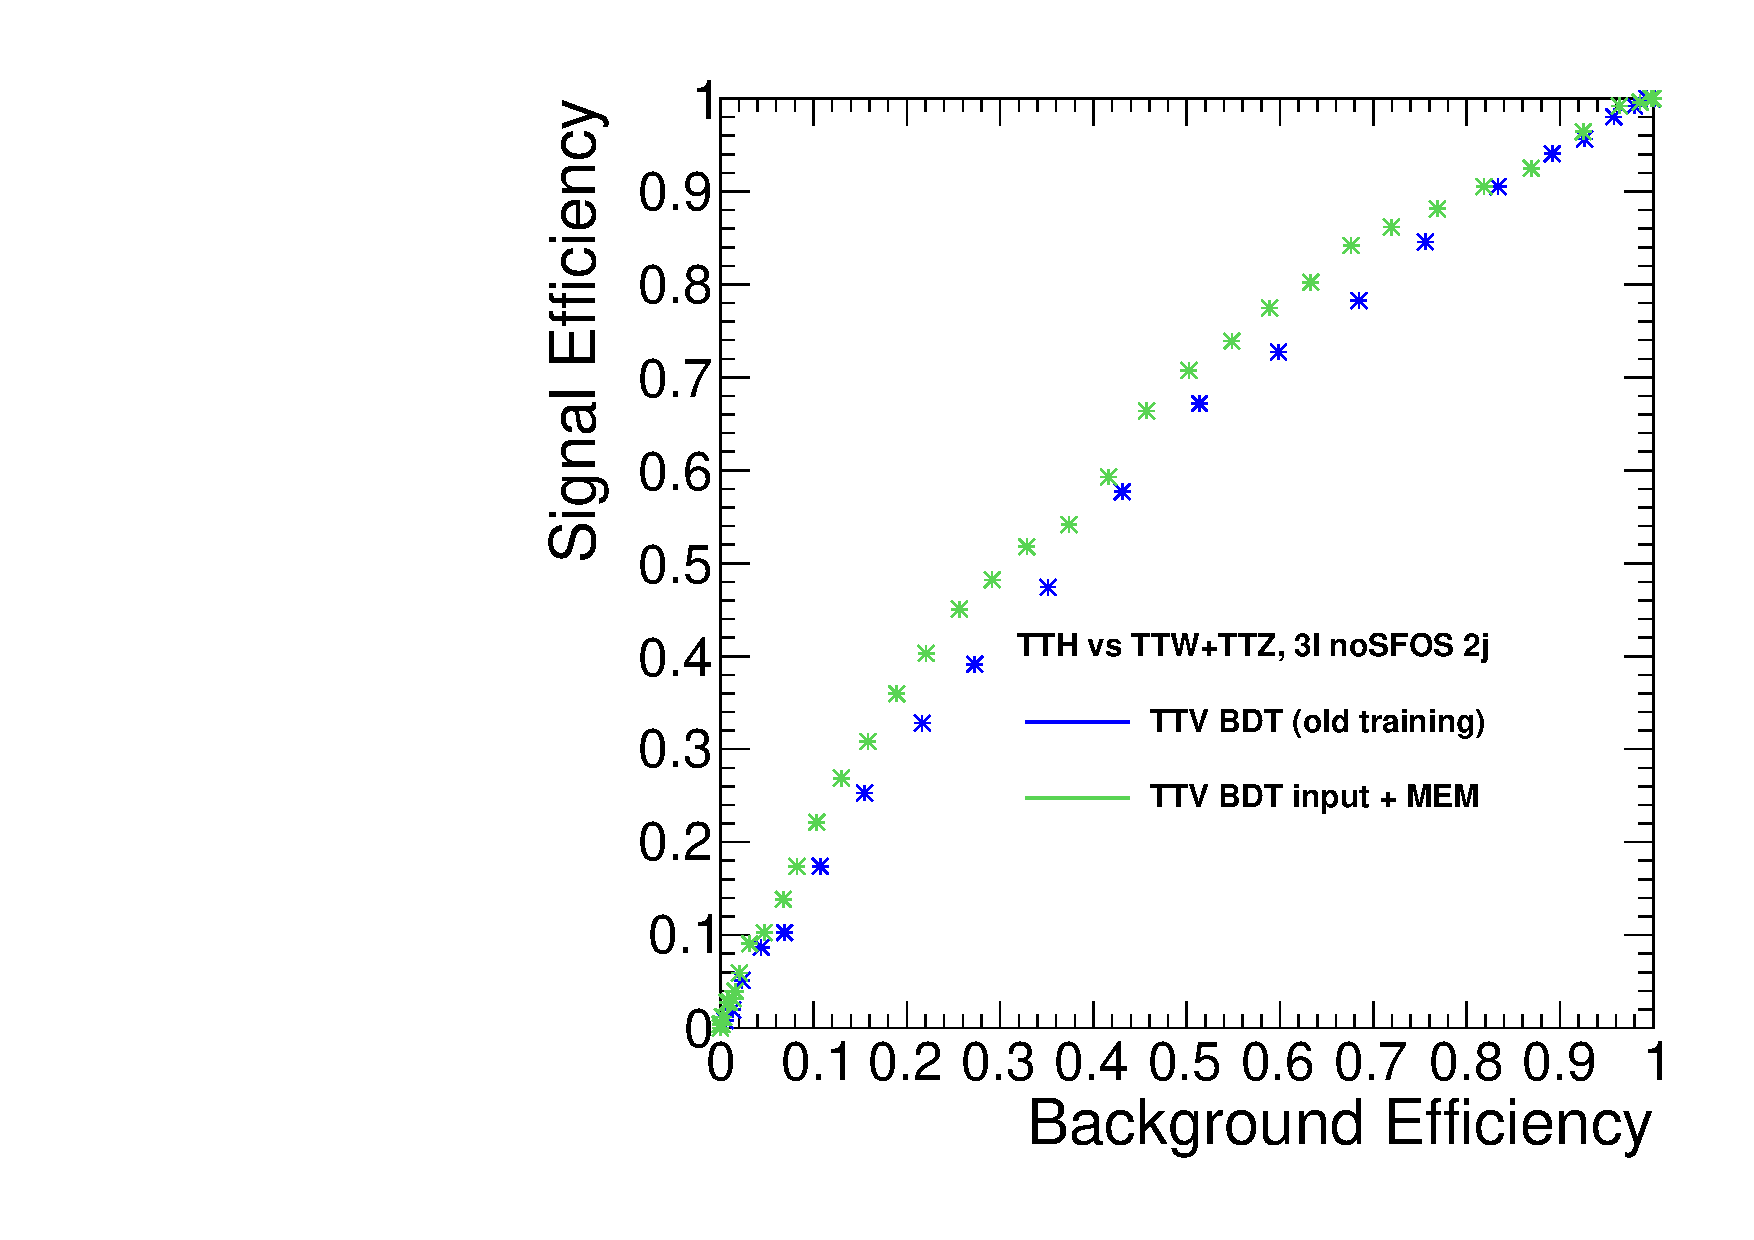
\includegraphics[width=0.4\textwidth]{plots_mem/Moriond2017/TTV/CompareBDT_3l_noSFOS_2j.pdf}
    \caption{ \textcolor{green}{Updated} Comparison of TTV BDT and new BDT including MEM in 3l signal region, without SFOS lepton pair, for (a) all events (b) 0 missing jets, (c) 1 missing jets, (d) 2 missing jets.}
  \label{mem:BDTMEMtraining3lnoSFOS}
\end{figure}

\begin{figure}[Htb]
 \centering
   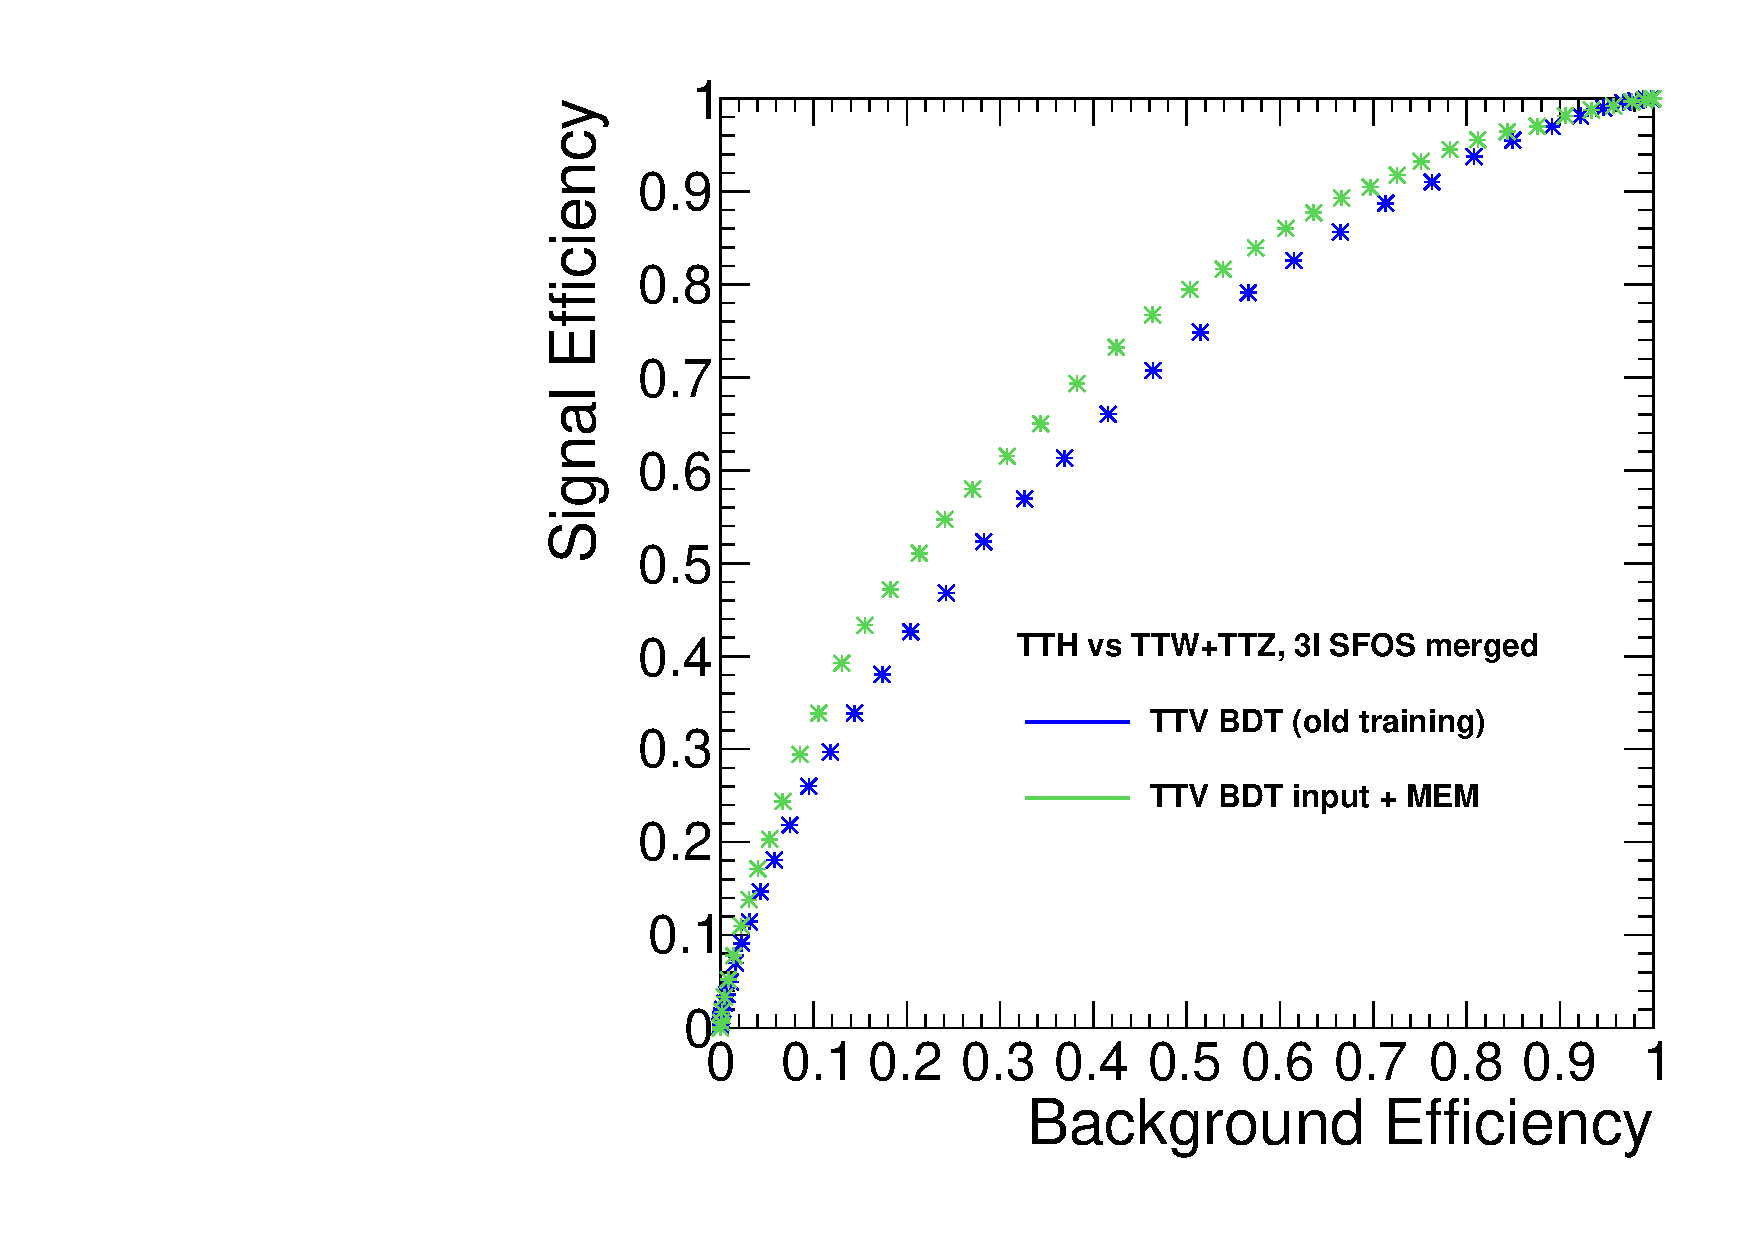
\includegraphics[width=0.4\textwidth]{plots_mem/Moriond2017/TTV/CompareBDT_3l_SFOS_merged.pdf}
   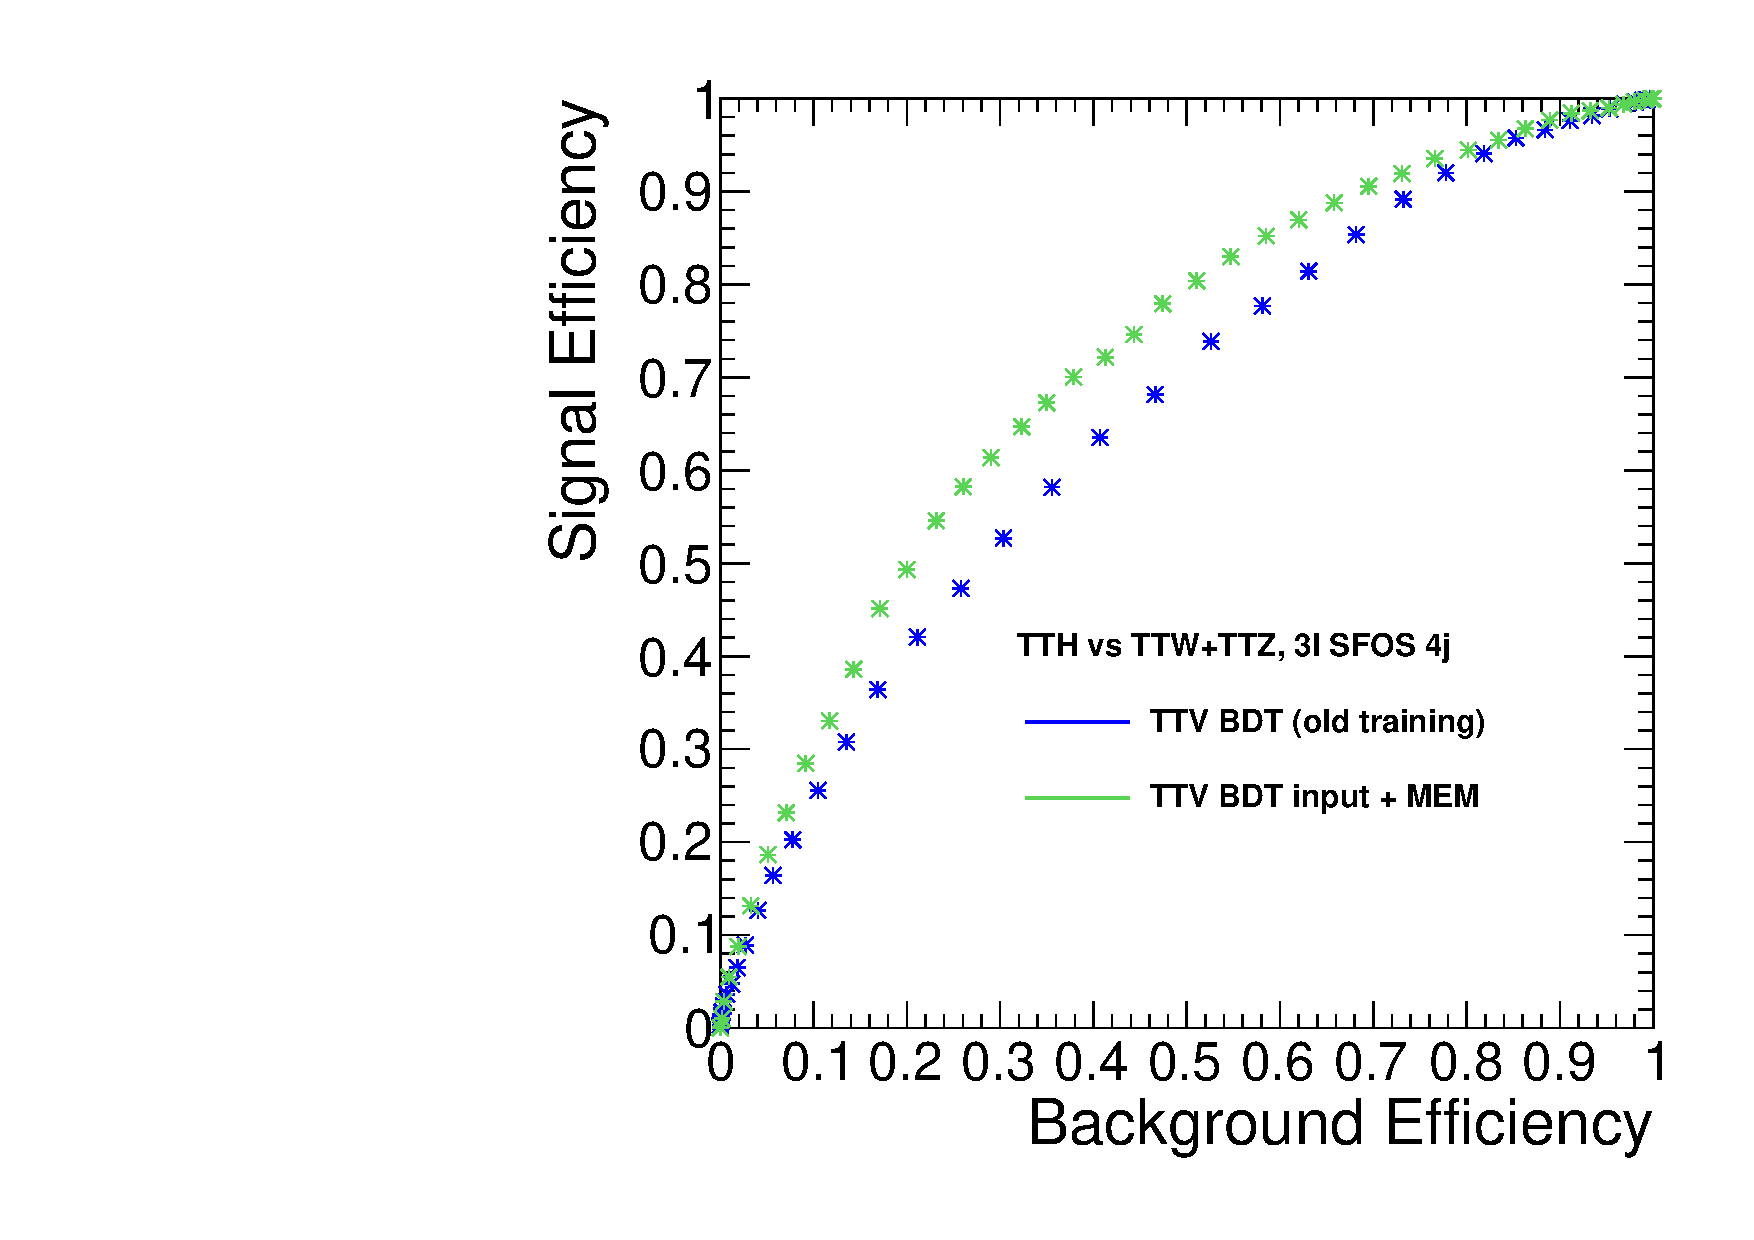
\includegraphics[width=0.4\textwidth]{plots_mem/Moriond2017/TTV/CompareBDT_3l_SFOS_4j.pdf}\\
   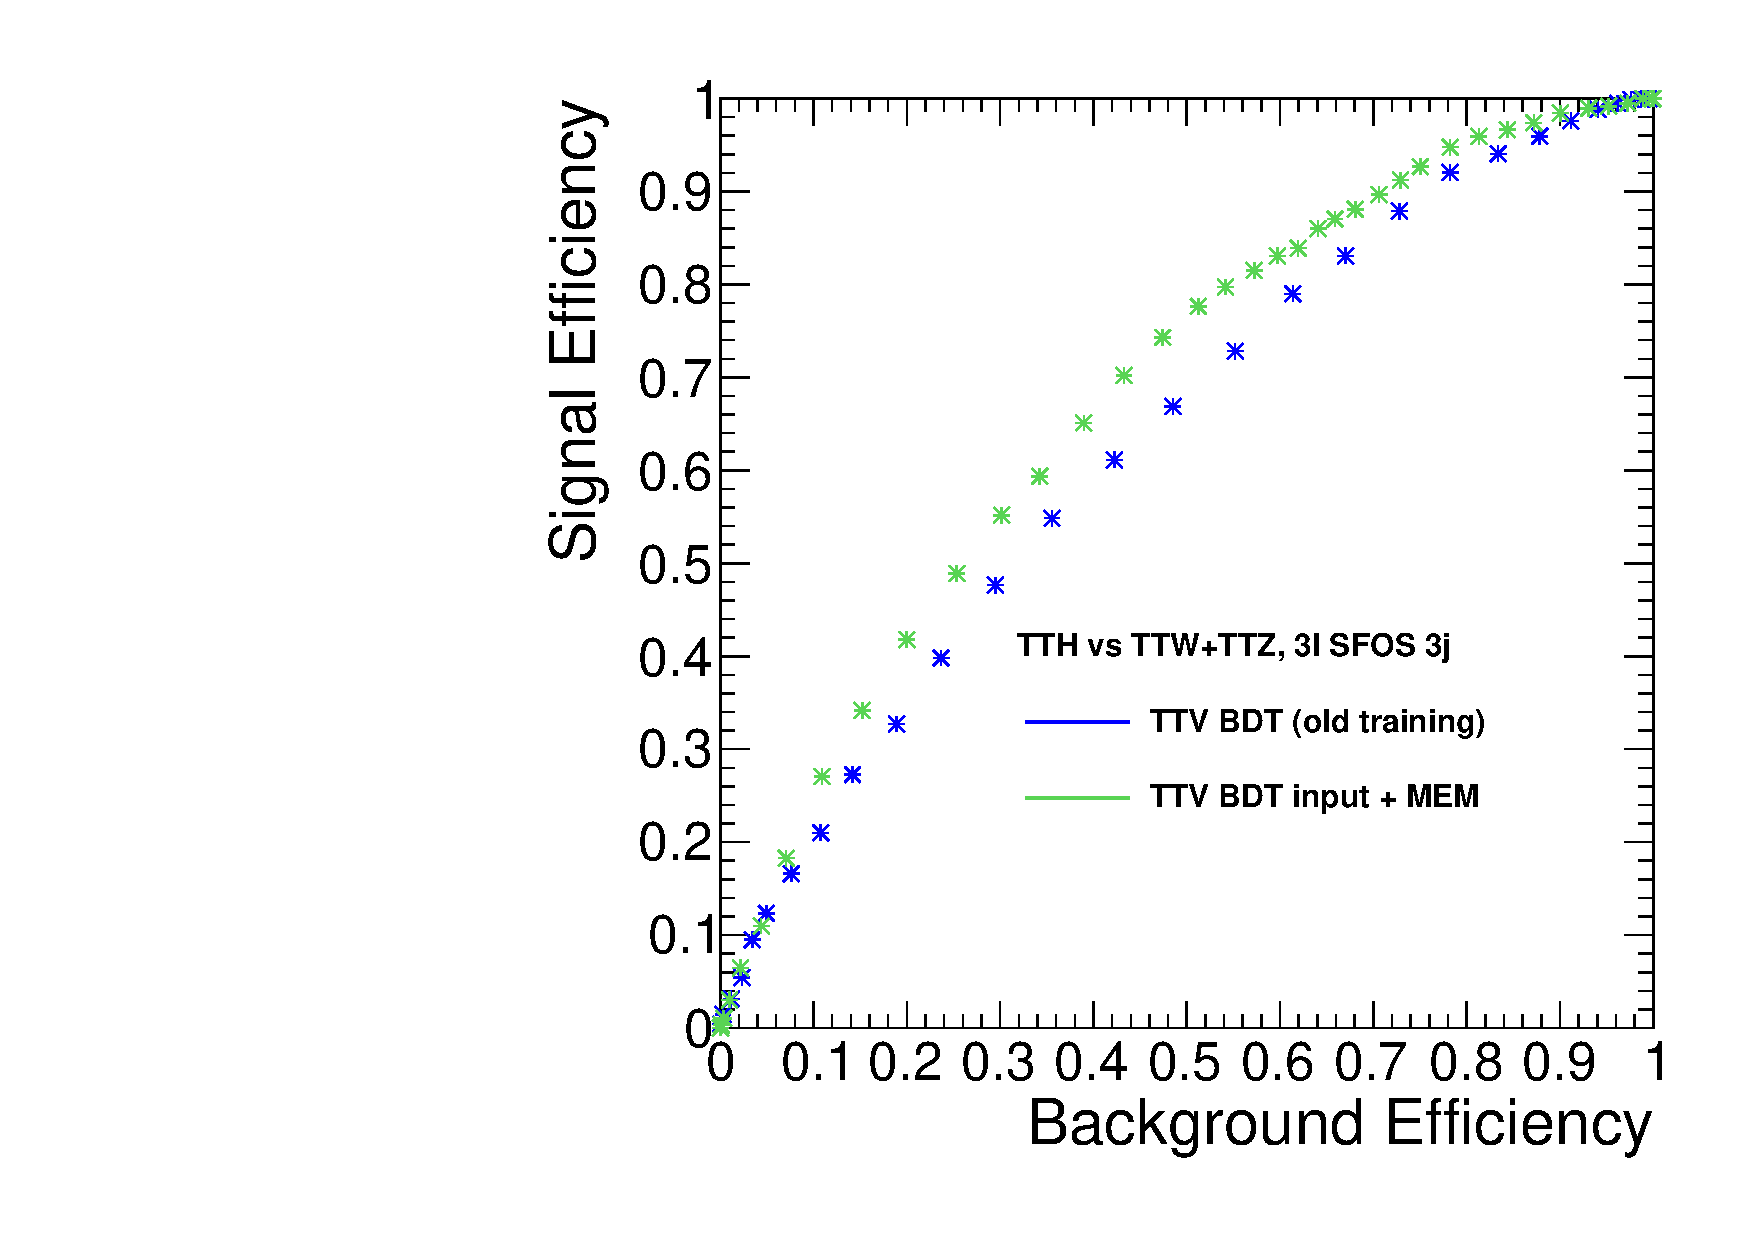
\includegraphics[width=0.4\textwidth]{plots_mem/Moriond2017/TTV/CompareBDT_3l_SFOS_3j.pdf}
   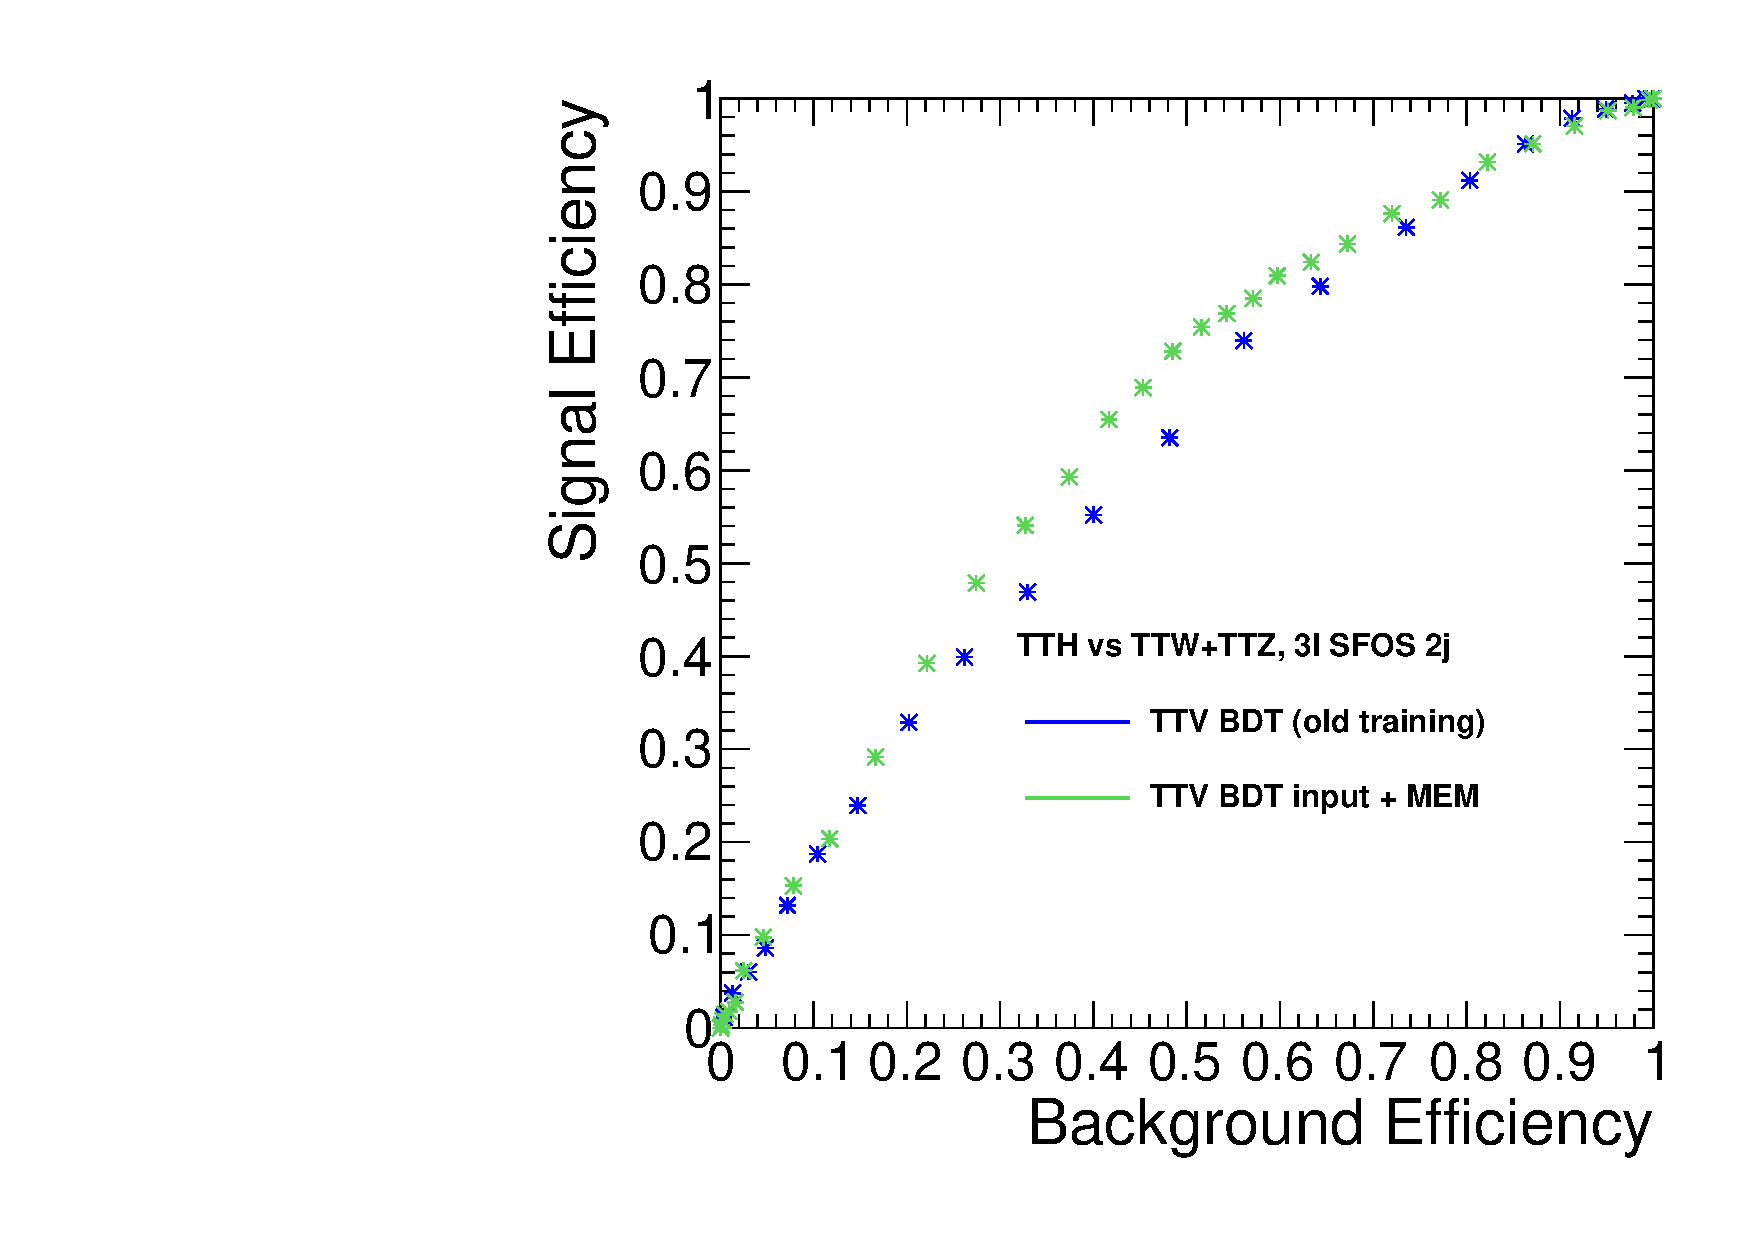
\includegraphics[width=0.4\textwidth]{plots_mem/Moriond2017/TTV/CompareBDT_3l_SFOS_2j.pdf}
   \caption{ \textcolor{green}{Updated} Comparison of TTV BDT and new BDT including MEM in 3l signal region, with a SFOS lepton pair, for (a) all events (b) 0 missing jets, (c) 1 missing jets, (d) 2 missing jets.}
  \label{mem:BDTMEMtraining3lSFOS}
\end{figure}

\begin{figure}[Htb]
 \centering
   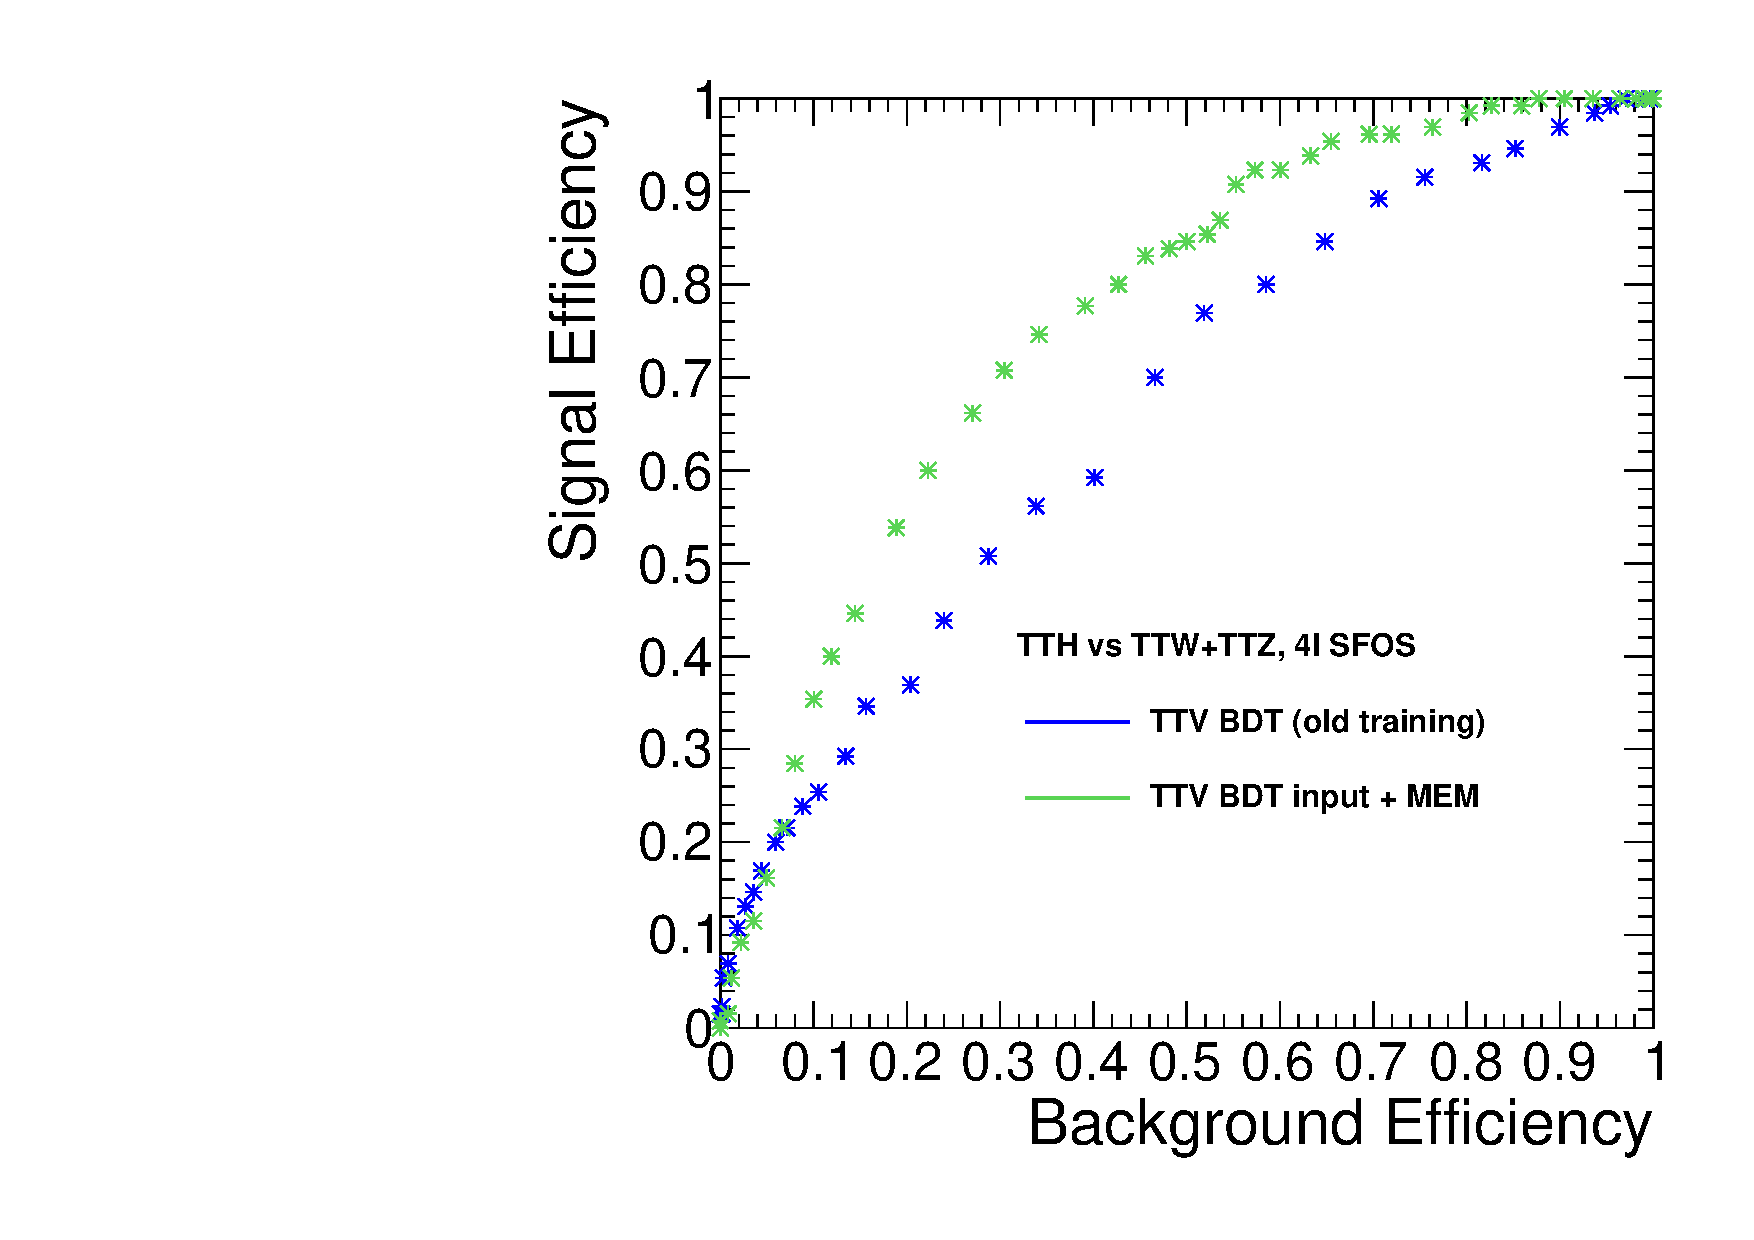
\includegraphics[width=0.4\textwidth]{plots_mem/Moriond2017/TTV/CompareBDT_4l_SFOS.pdf}
   \caption{ \textcolor{green}{Updated} Comparison of TTV BDT and new BDT including MEM in 4l signal region for all events}
  \label{mem:BDTMEMtraining4l}
\end{figure}

\subsubsection*{Comparison with TT BDT}

The performance of MEM discriminants is compared on fig.~\ref{mem:comparisonBDT2lssTT} for 2lss categories and fig.~\ref{mem:comparisonBDT3lTT} for 3l categories. Performance is in any case comparable, slightly lower in 2lss categories, and equivalent or slighlty better in 3l categories. The performance is better for categories where all the jets are reconstructed. There is almost no discrimination when 2 jets are missing, which is also the case for the TTV BDT.

\begin{figure}[Htb]
 \centering
   \includegraphics[width=0.4\textwidth]{plots_mem/Moriond2017/TTbar/CompareBDTvsMEM_2l_merged.pdf}\\
%   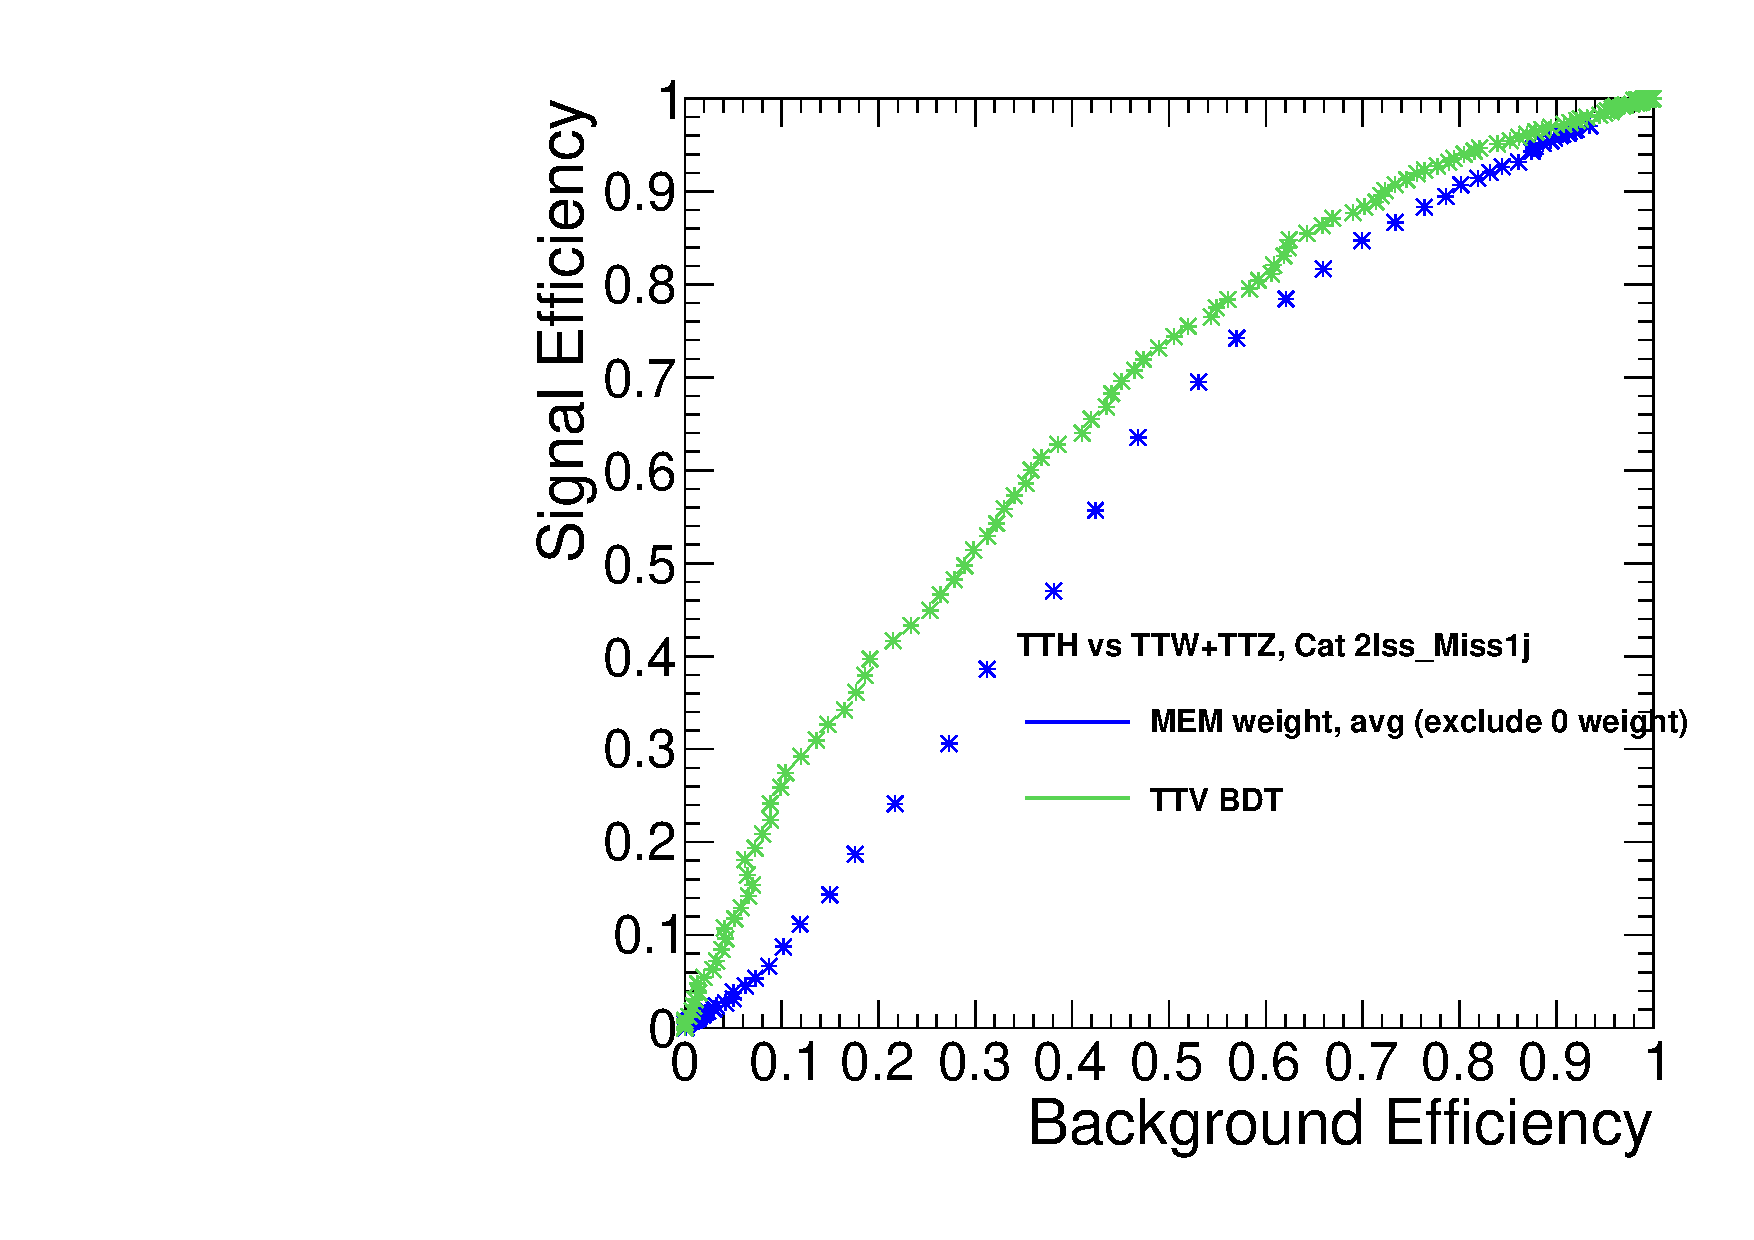
\includegraphics[width=0.4\textwidth]{plots_mem/EffSvsRejB_TTHvsTTVfull_catJets2lss_Miss1j_BDT.pdf}
%   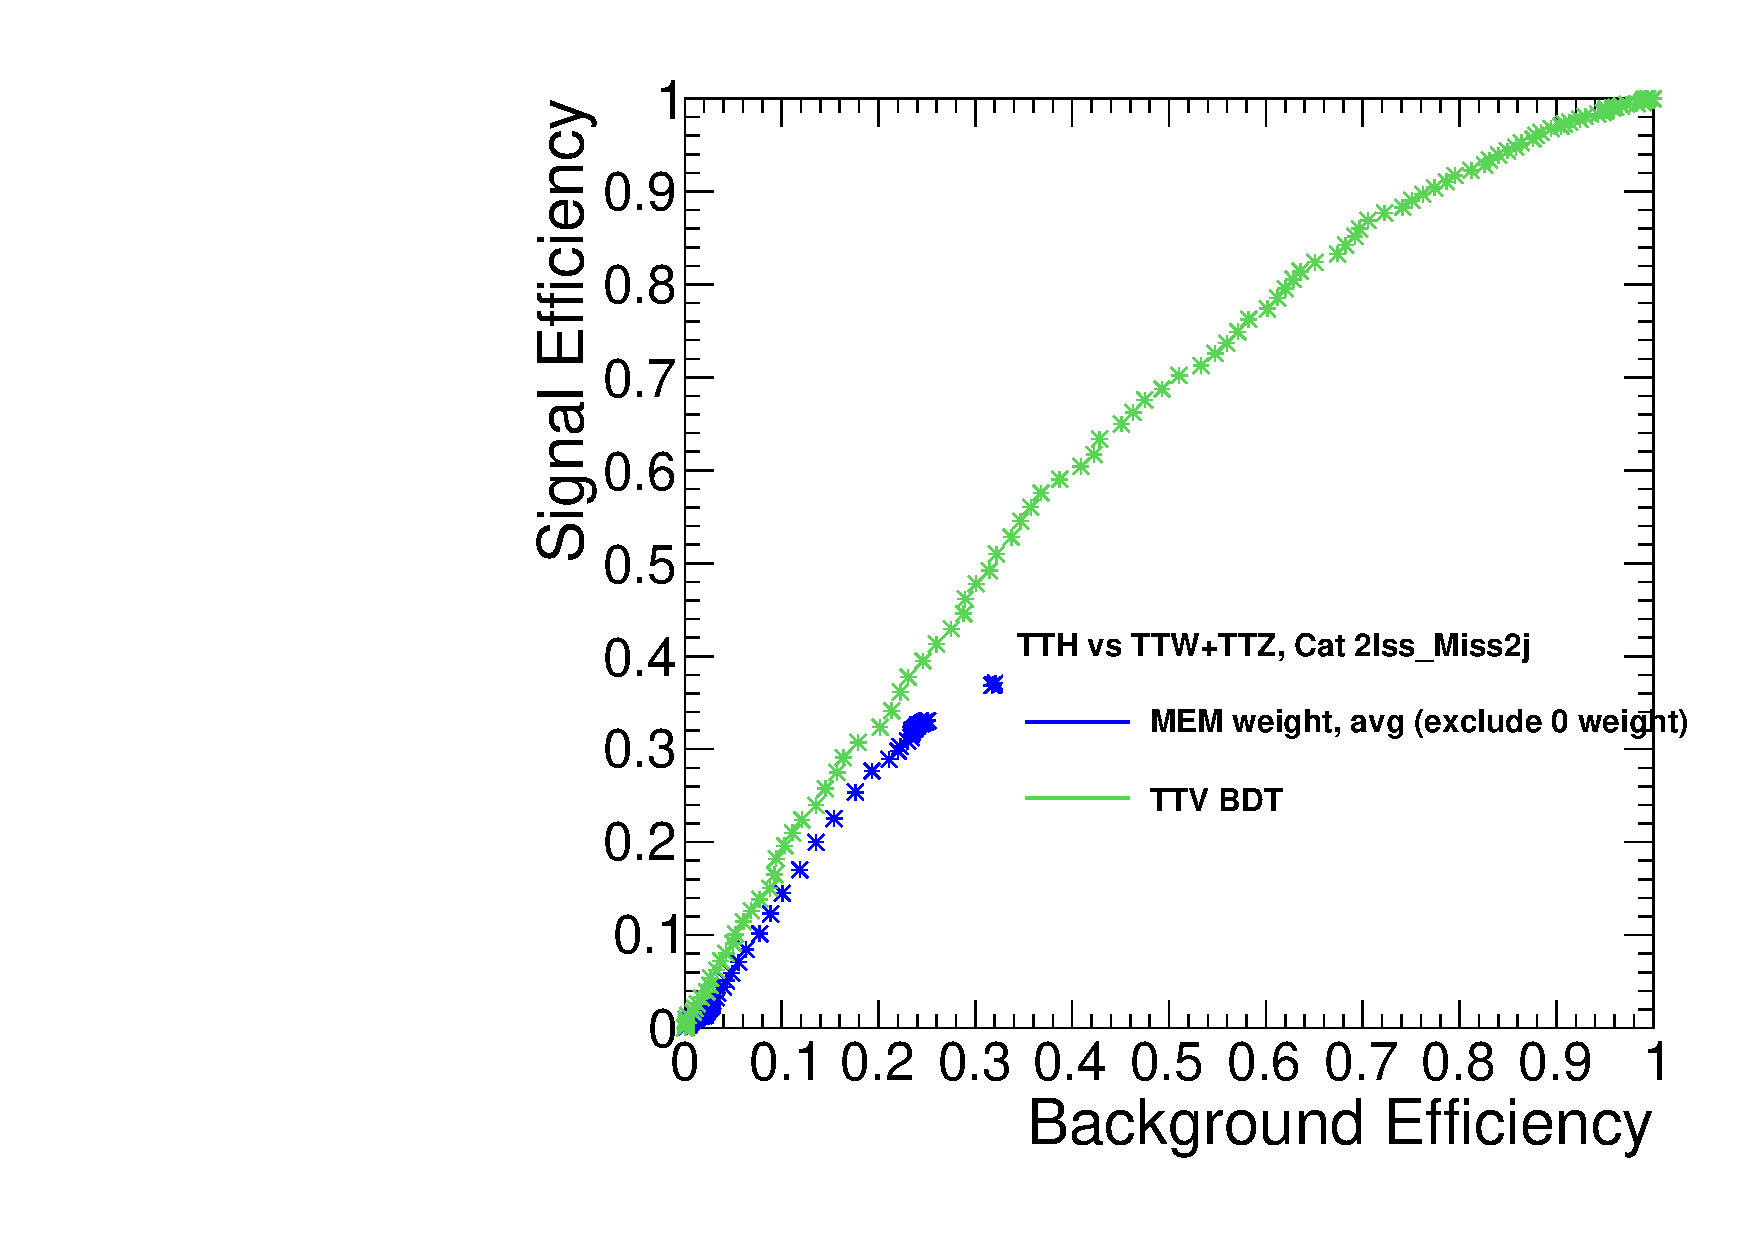
\includegraphics[width=0.4\textwidth]{plots_mem/EffSvsRejB_TTHvsTTVfull_catJets2lss_Miss2j_BDT.pdf}
   \caption{ \textcolor{green}{Updated} Comparison of MEM discriminants in 2lss signal region (merged).}
% for (a) 0 missing jets, (b) 1 missing jets, (c) 2 missing jets.}
  \label{mem:comparisonBDT2lssTT}
\end{figure}

\begin{figure}[Htb]
 \centering
   \includegraphics[width=0.4\textwidth]{plots_mem/Moriond2017/TTbar/CompareBDTvsMEM_3l_merged.pdf}\\
%   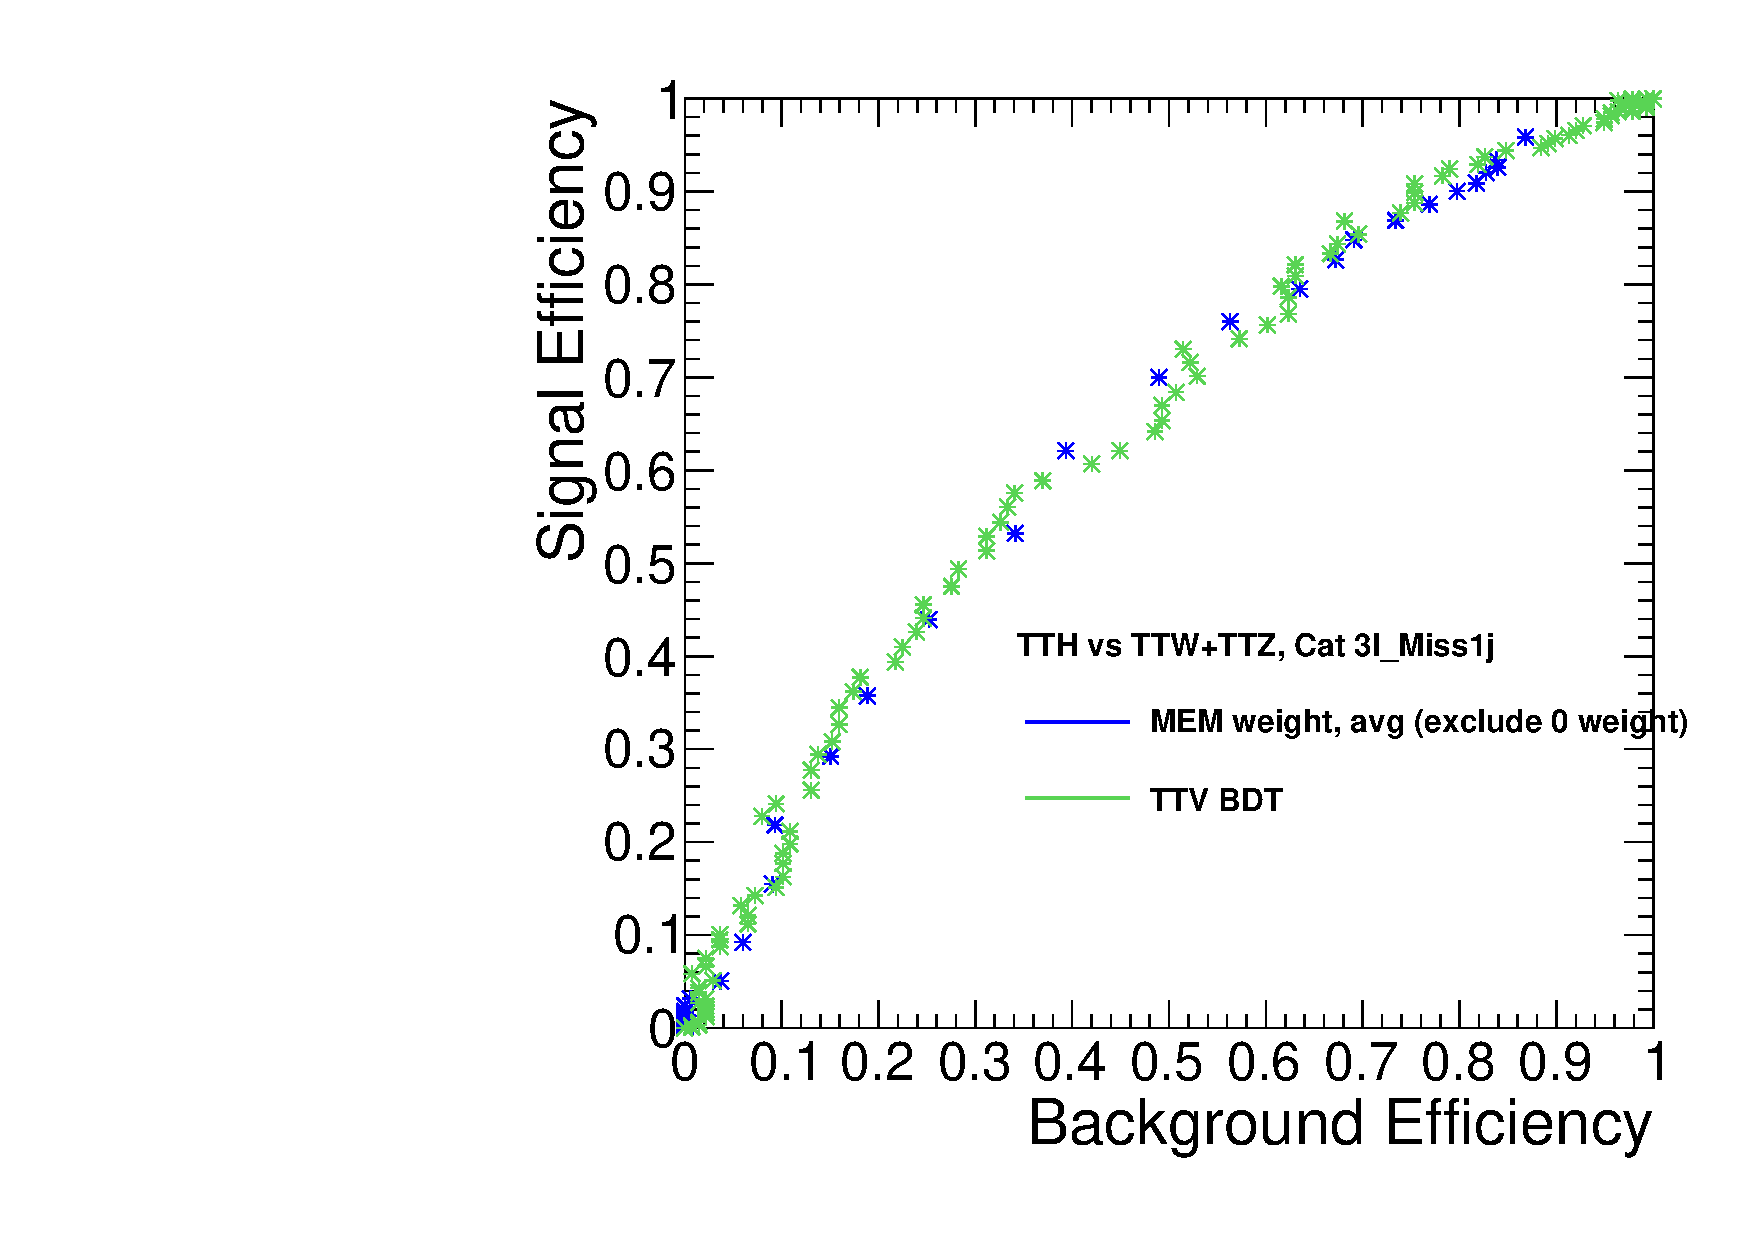
\includegraphics[width=0.4\textwidth]{plots_mem/EffSvsRejB_TTHvsTTVfull_catJets3l_Miss1j_BDT.pdf}
%   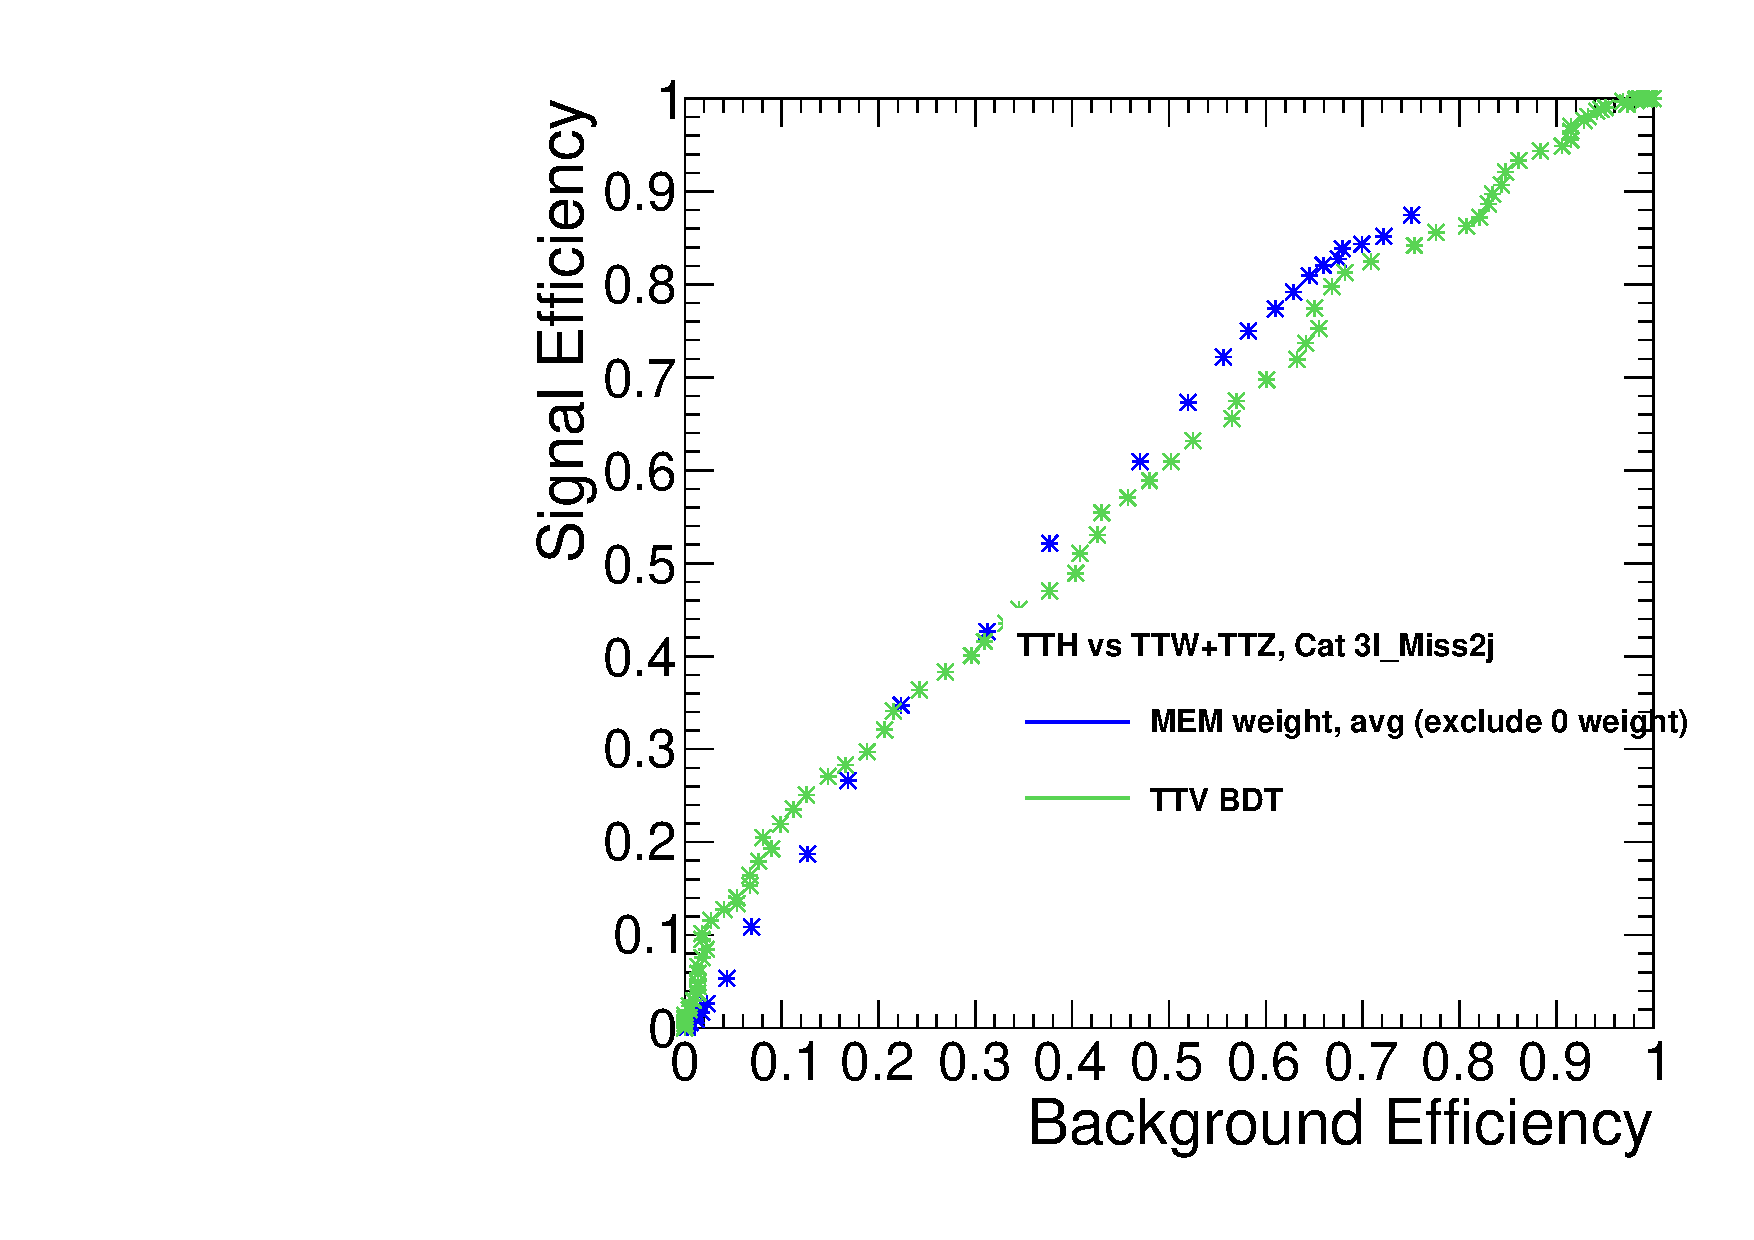
\includegraphics[width=0.4\textwidth]{plots_mem/EffSvsRejB_TTHvsTTVfull_catJets3l_Miss2j_BDT.pdf}
  \caption{ \textcolor{green}{Updated} Comparison of MEM discriminants in 3l signal region (merged).}
% for (a) 0 missing jets, (b) 1 missing jets, (c) 2 missing jets.}
  \label{mem:comparisonBDT3lTT}
\end{figure}

\subsection*{MEM as input variable to the TT BDT}\label{sec:meminputttbar}

Given that the performances of TT BDT and MEM discriminants are similar, it makes sense to train BDT including the MEM.
We train new BDT's using Madgraph $t\bar{t}$ large samples with same setup used for training BDT TT, but including MEM weights. Three trainings are performed:
\begin{itemize}
\item 2lss category: TT BDT inputs + $log(w_{TTH})$ + $log(w_{TTW})$ + weight of the ttH fully leptonic and semi leptonic reconstruction
\item 3l/4l categories with a SFOS lepton pair: TT BDT inputs + $log(w_{TTH})$ + $log(w_{TT})$
\end{itemize}
The $log(w)$ are the $log$ of average MEM weight excluding null weights.

Results are shown on fig.\ref{mem:BDTMEMtraining2lss} for 2lss category, fig.\ref{mem:BDTMEMtraining3lnoSFOS} for 3l without SFOS lepton pair, fig.~\ref{mem:BDTMEMtraining3lSFOS} for 3l with a SFOS lepton pair, and fig.~\ref{mem:BDTMEMtraining4l} for 4l. Performance of BDT including MEM is greater than the previous training of TTV BDT for all categories, by a few \% in signal efficiency for a given background rejection in 2lss categories and up to 10-15\% in 3l and 4l categories.

\begin{figure}[Htb]
 \centering
   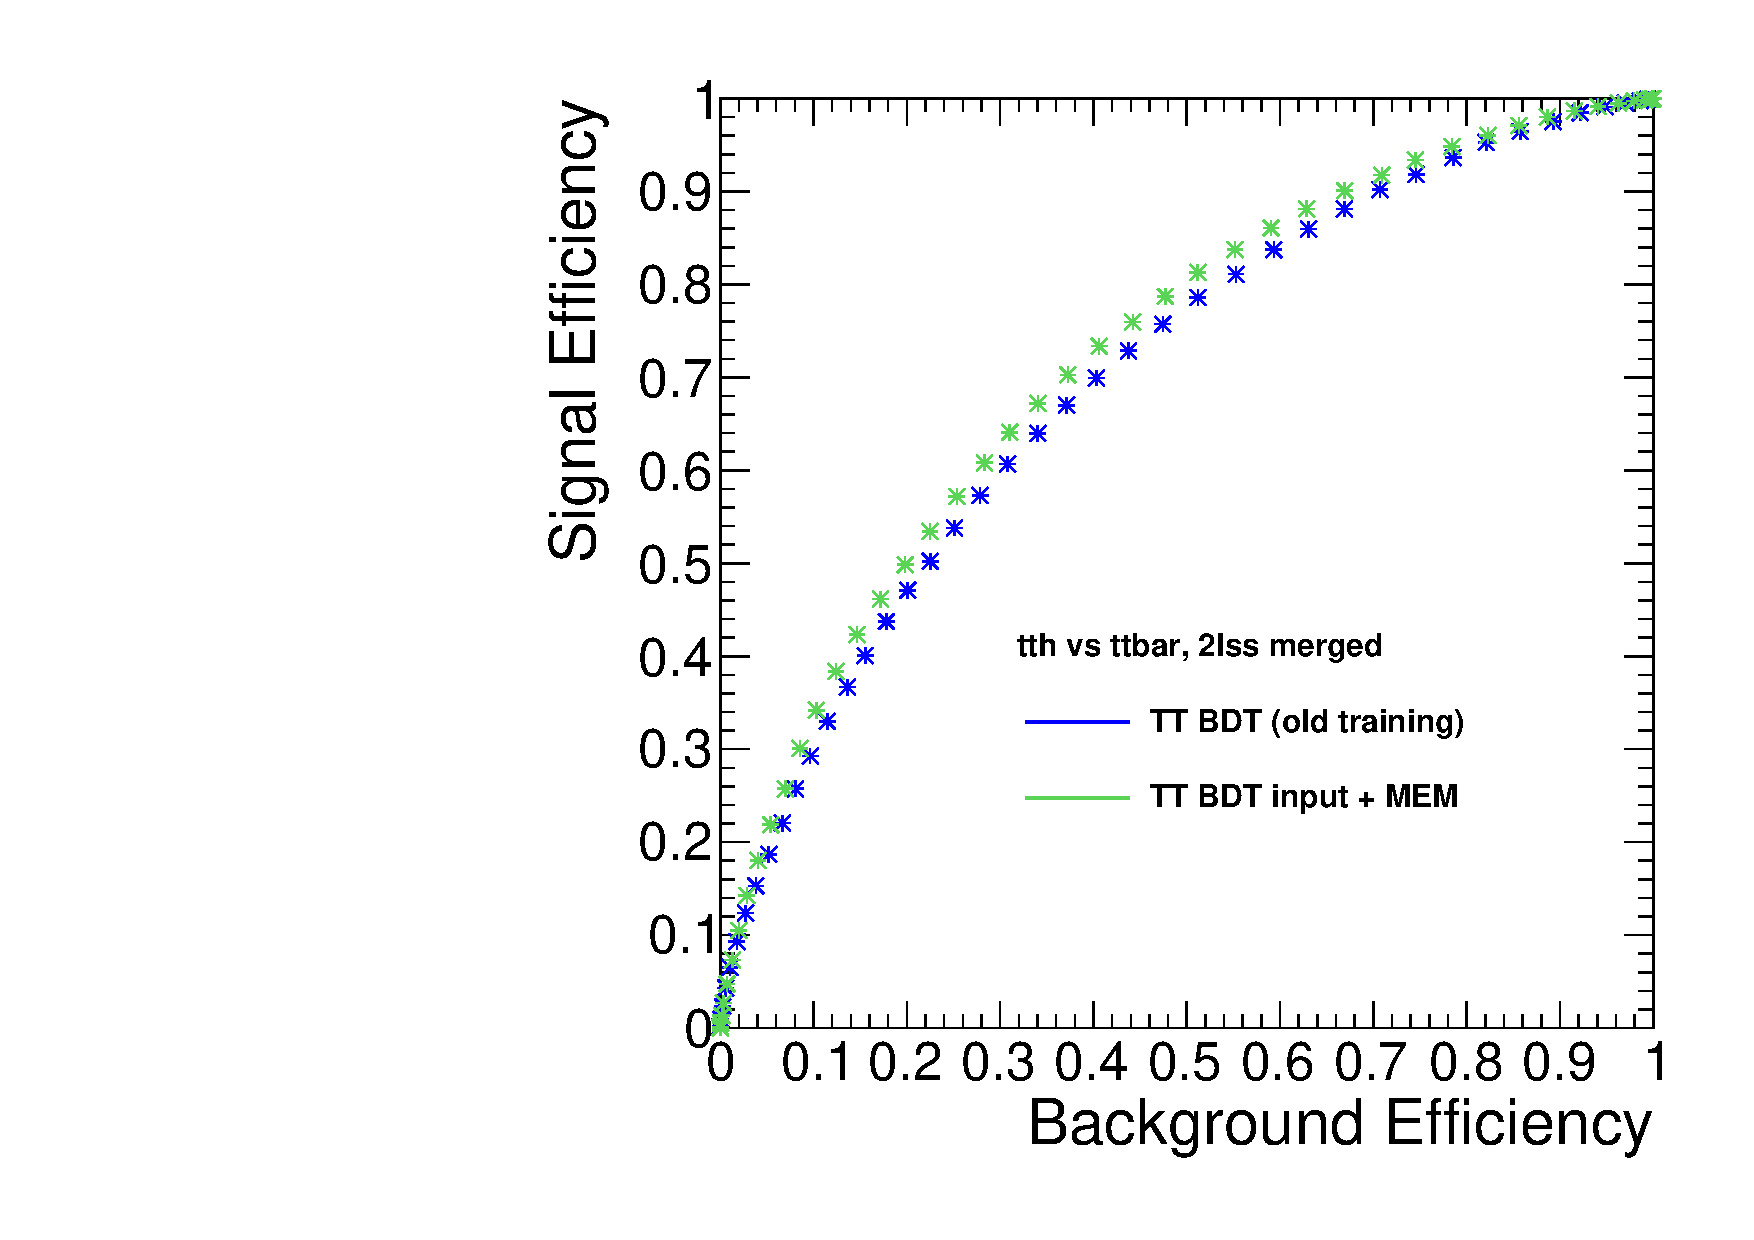
\includegraphics[width=0.4\textwidth]{plots_mem/Moriond2017/TTbar/CompareBDT_TT_2lss_merged.pdf}\\
   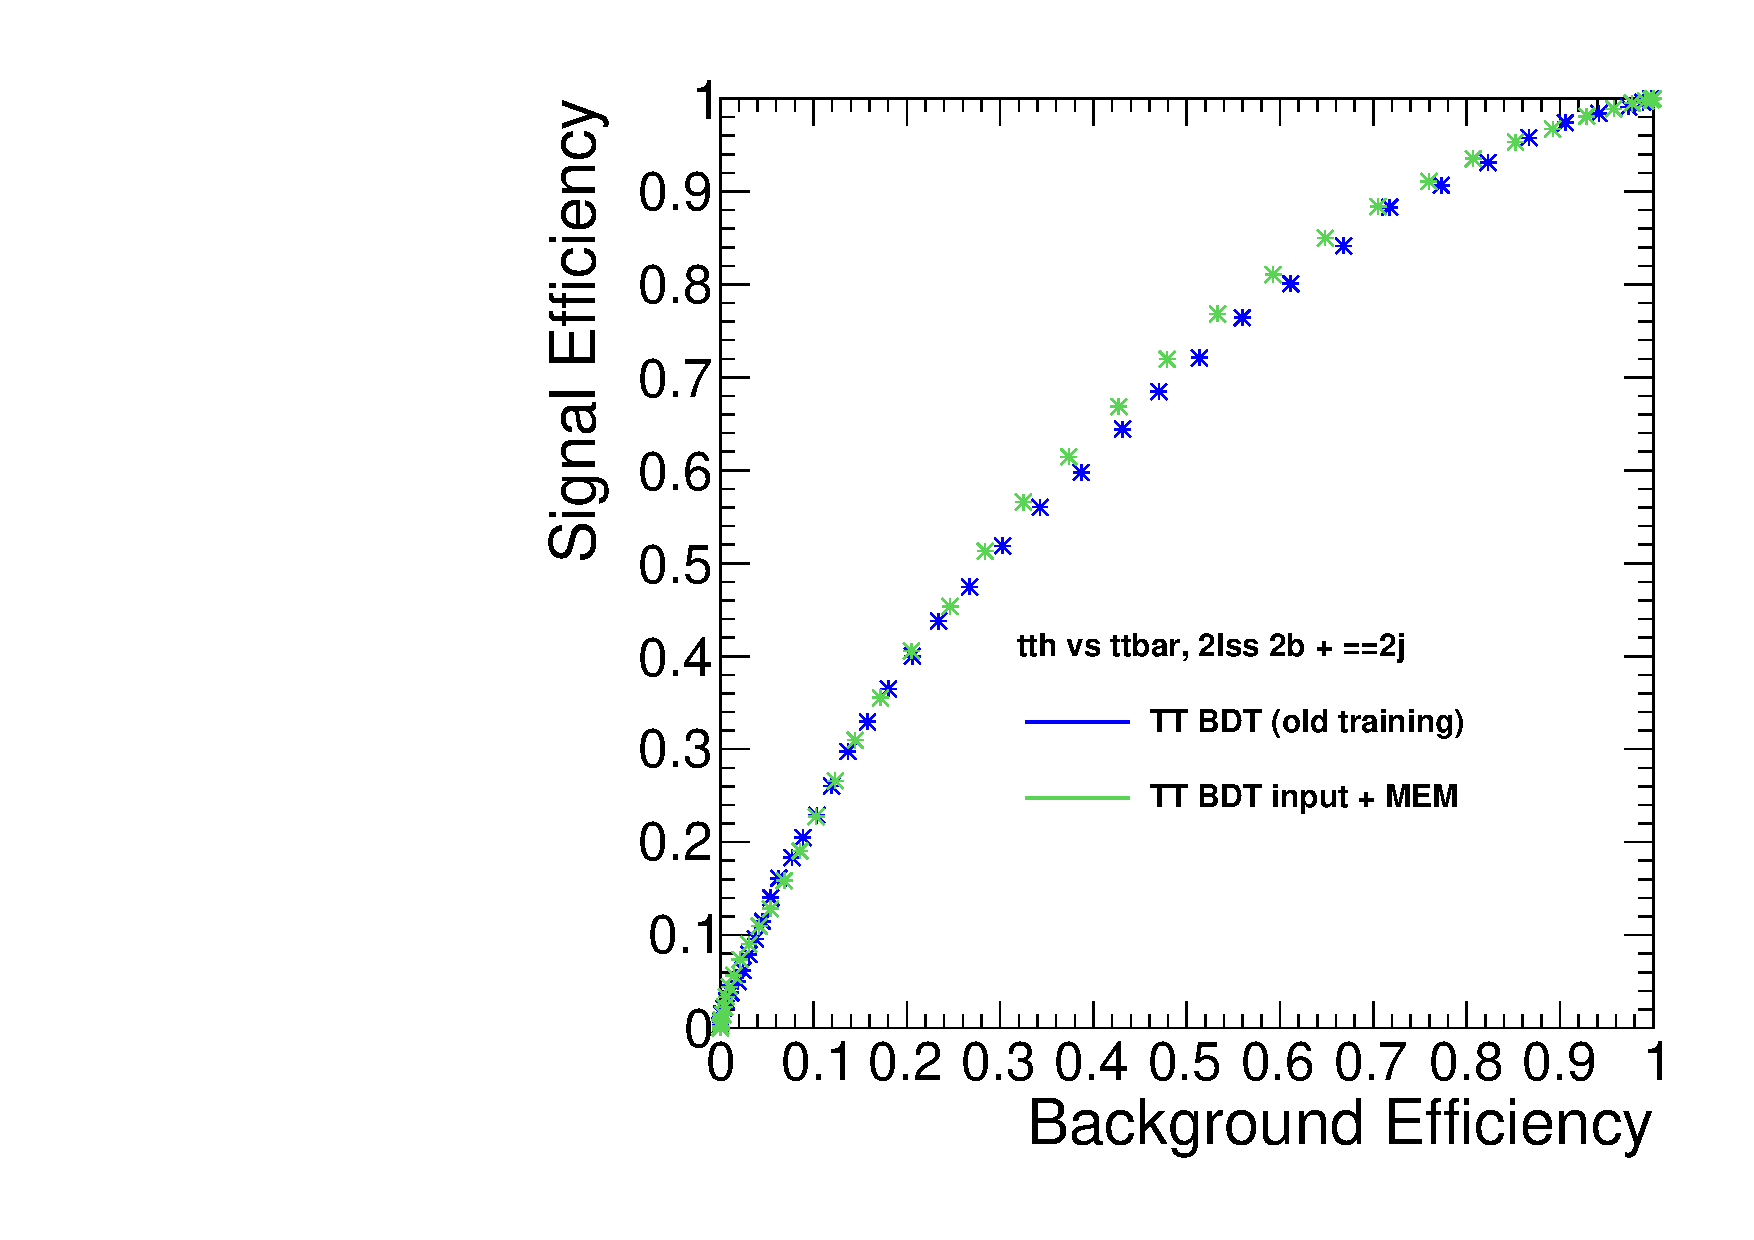
\includegraphics[width=0.4\textwidth]{plots_mem/Moriond2017/TTbar/CompareBDT_2lss_1b_3j.pdf}
   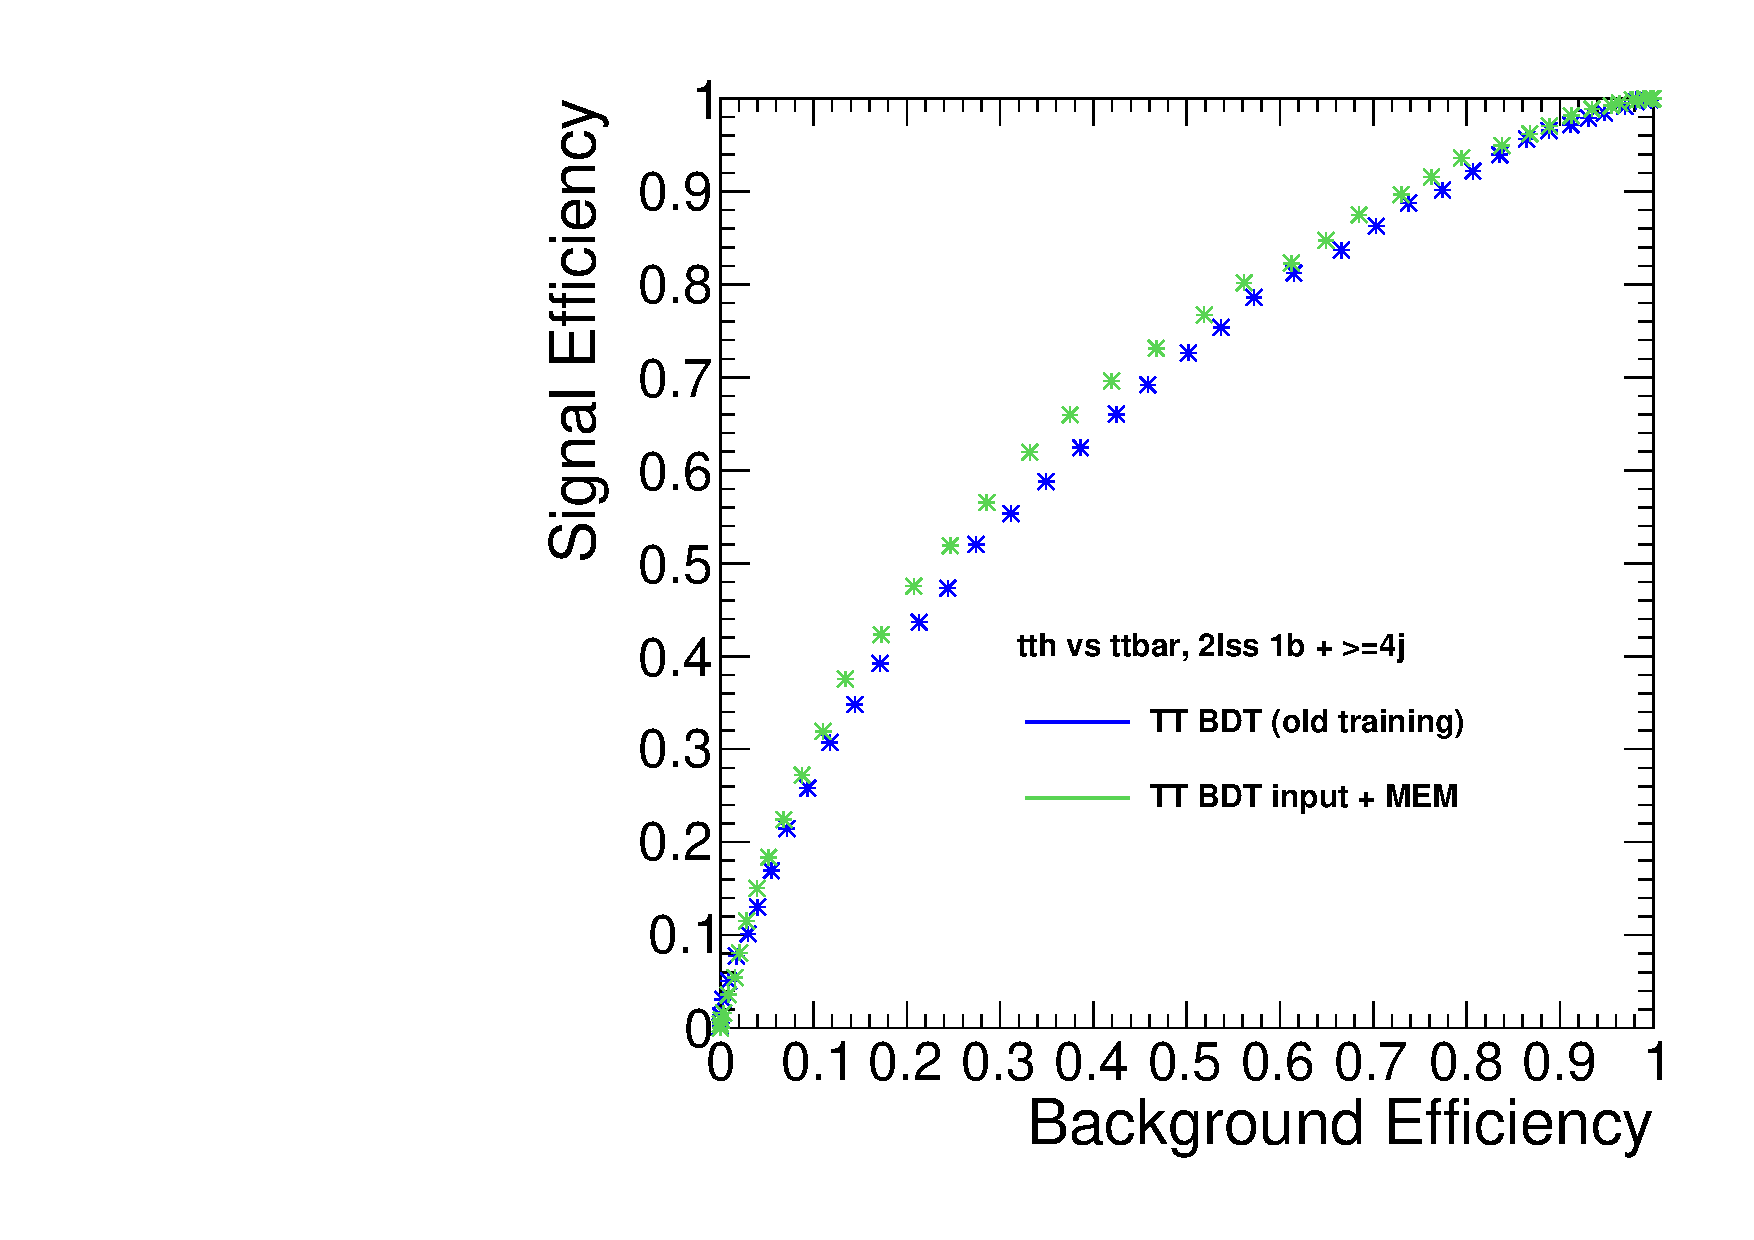
\includegraphics[width=0.4\textwidth]{plots_mem/Moriond2017/TTbar/CompareBDT_2lss_1b_4j.pdf} \\
   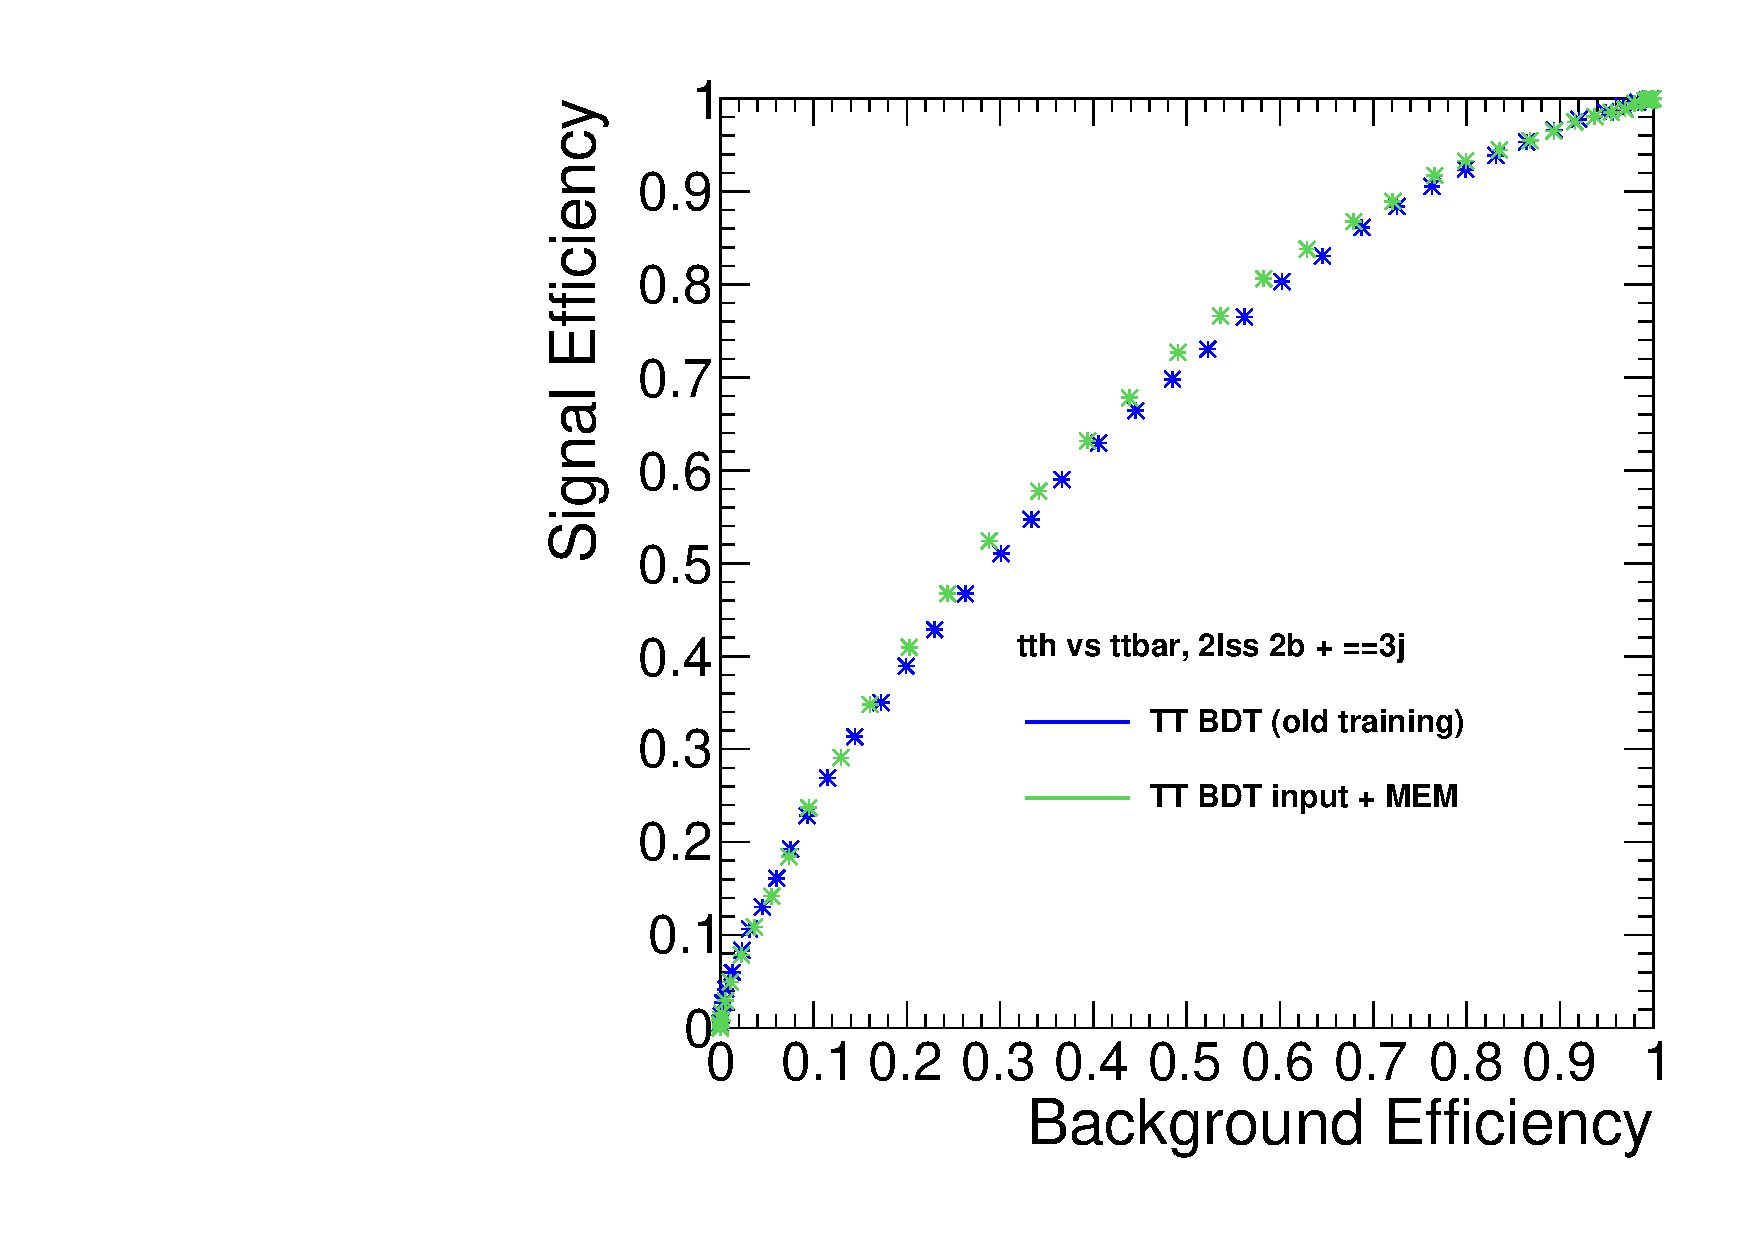
\includegraphics[width=0.4\textwidth]{plots_mem/Moriond2017/TTbar/CompareBDT_2lss_2b_3j.pdf}
   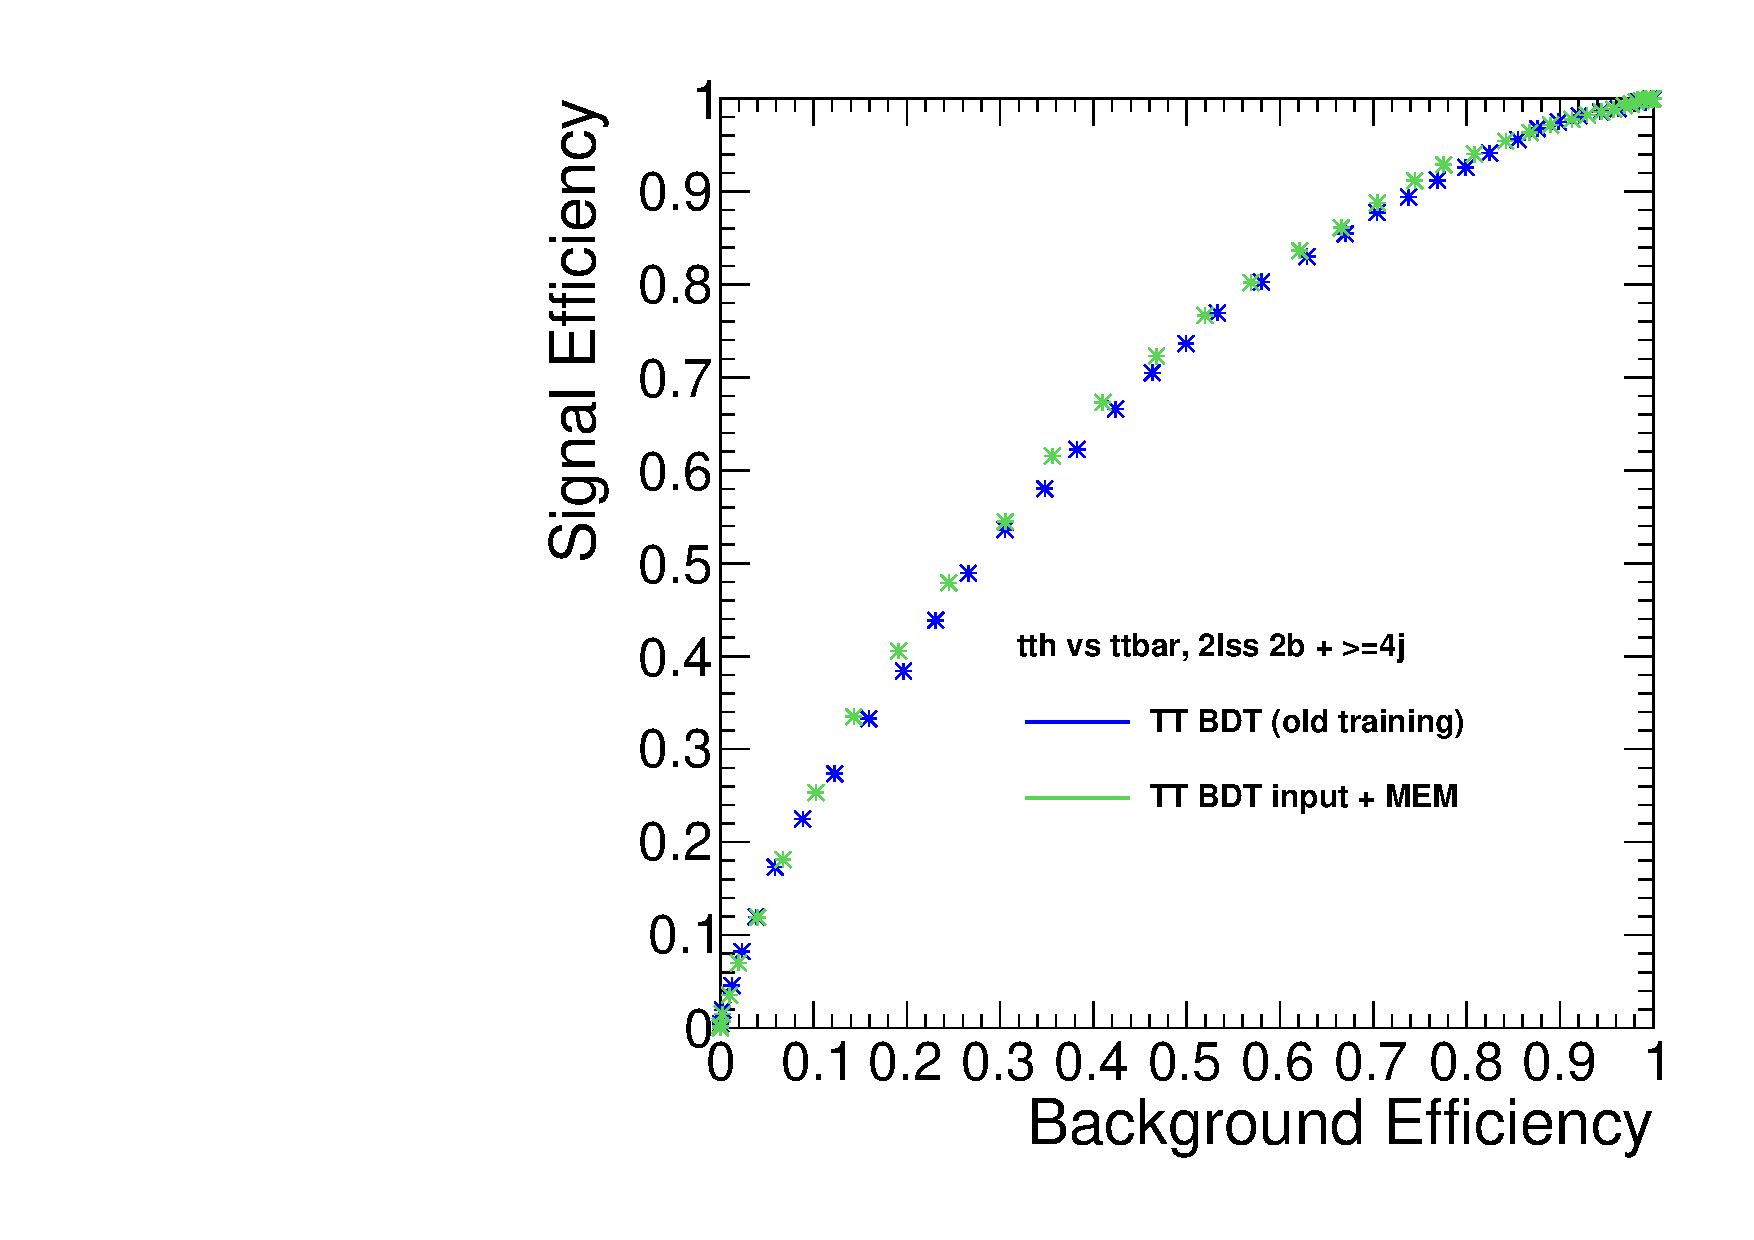
\includegraphics[width=0.4\textwidth]{plots_mem/Moriond2017/TTbar/CompareBDT_2lss_2b_4j.pdf}
   \caption{ \textcolor{green}{Updated} Comparison of TT BDT and new BDT including MEM in 2lss signal region for (a) all events (b) 0 missing jets, (c) 1 missing jets, (d) 2 missing jets.}
  \label{mem:BDTMEMtraining2lss}
\end{figure}

\begin{figure}[Htb]
 \centering
   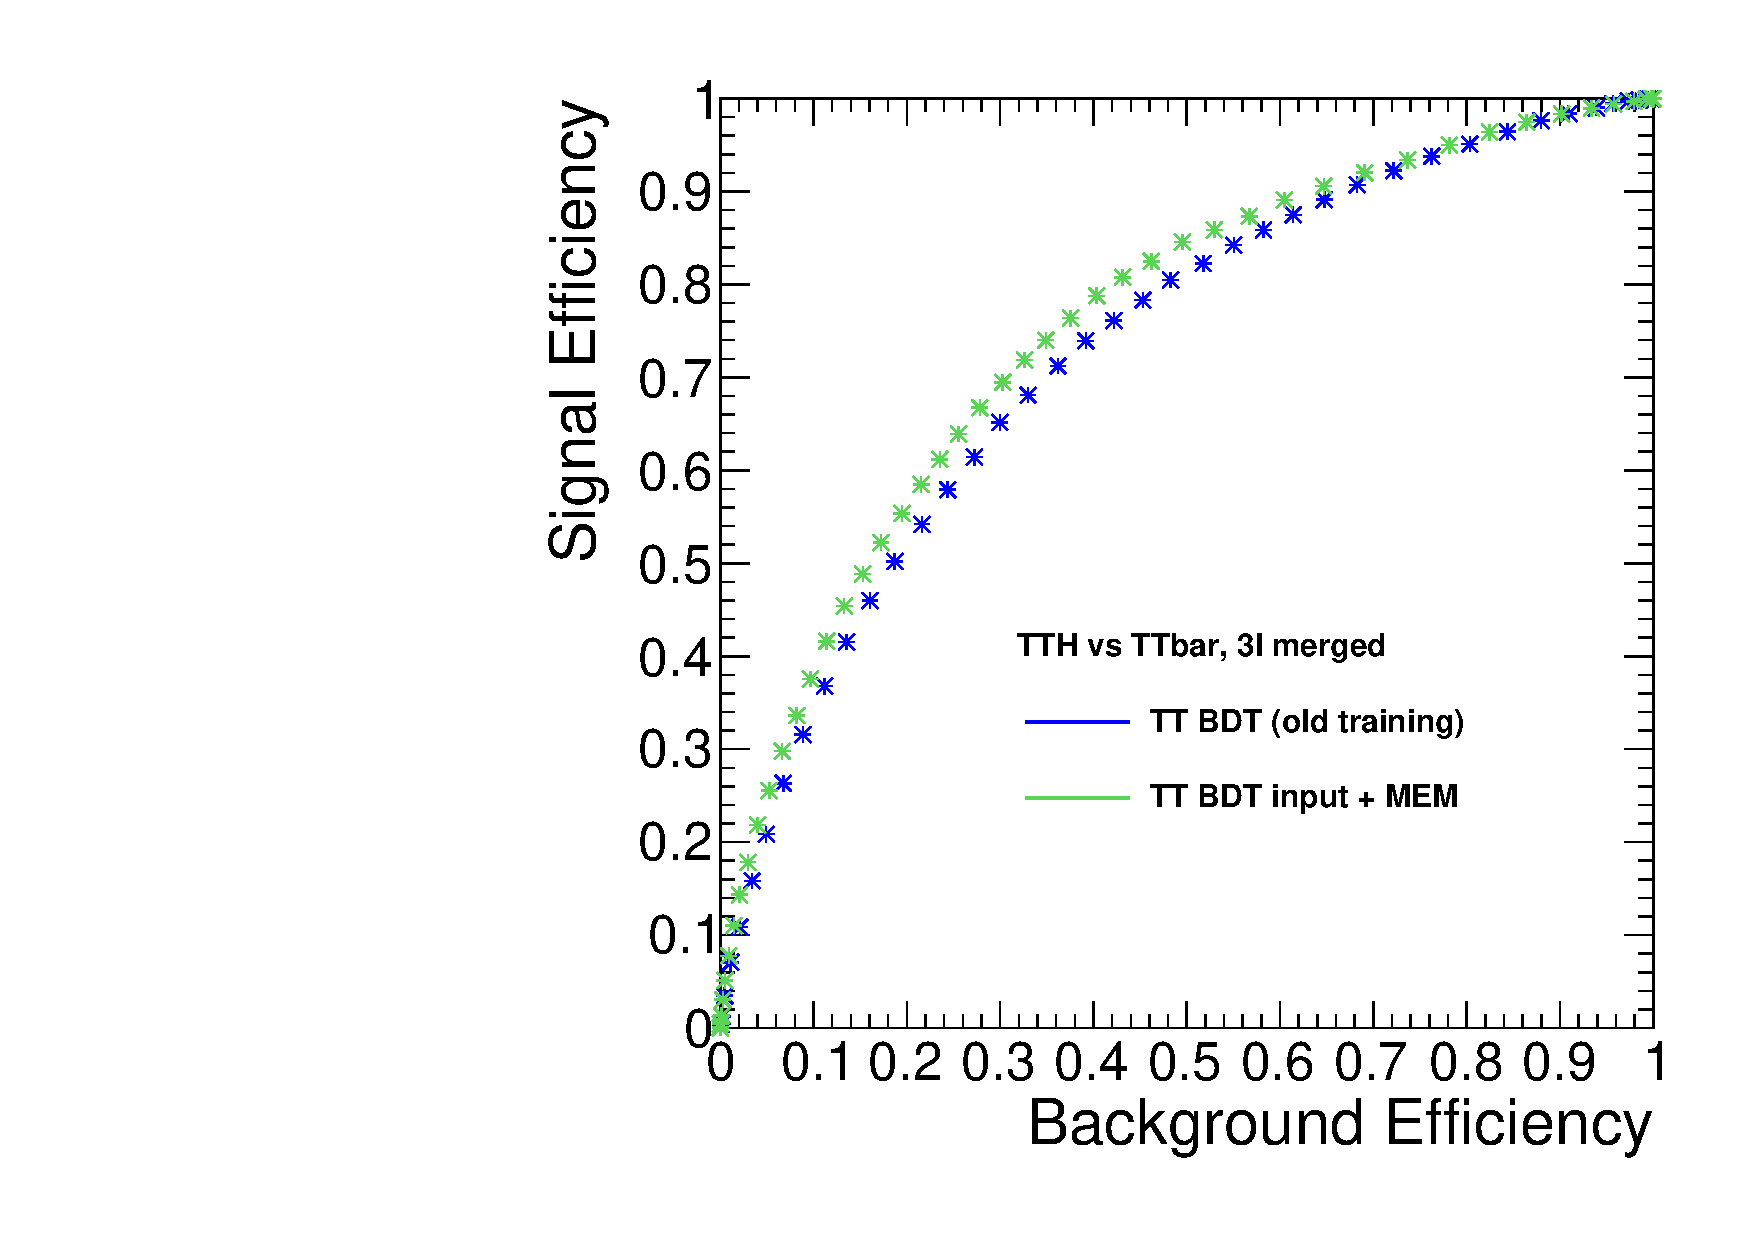
\includegraphics[width=0.4\textwidth]{plots_mem/Moriond2017/TTbar/CompareBDT_TT_3l_merged.pdf} \\
   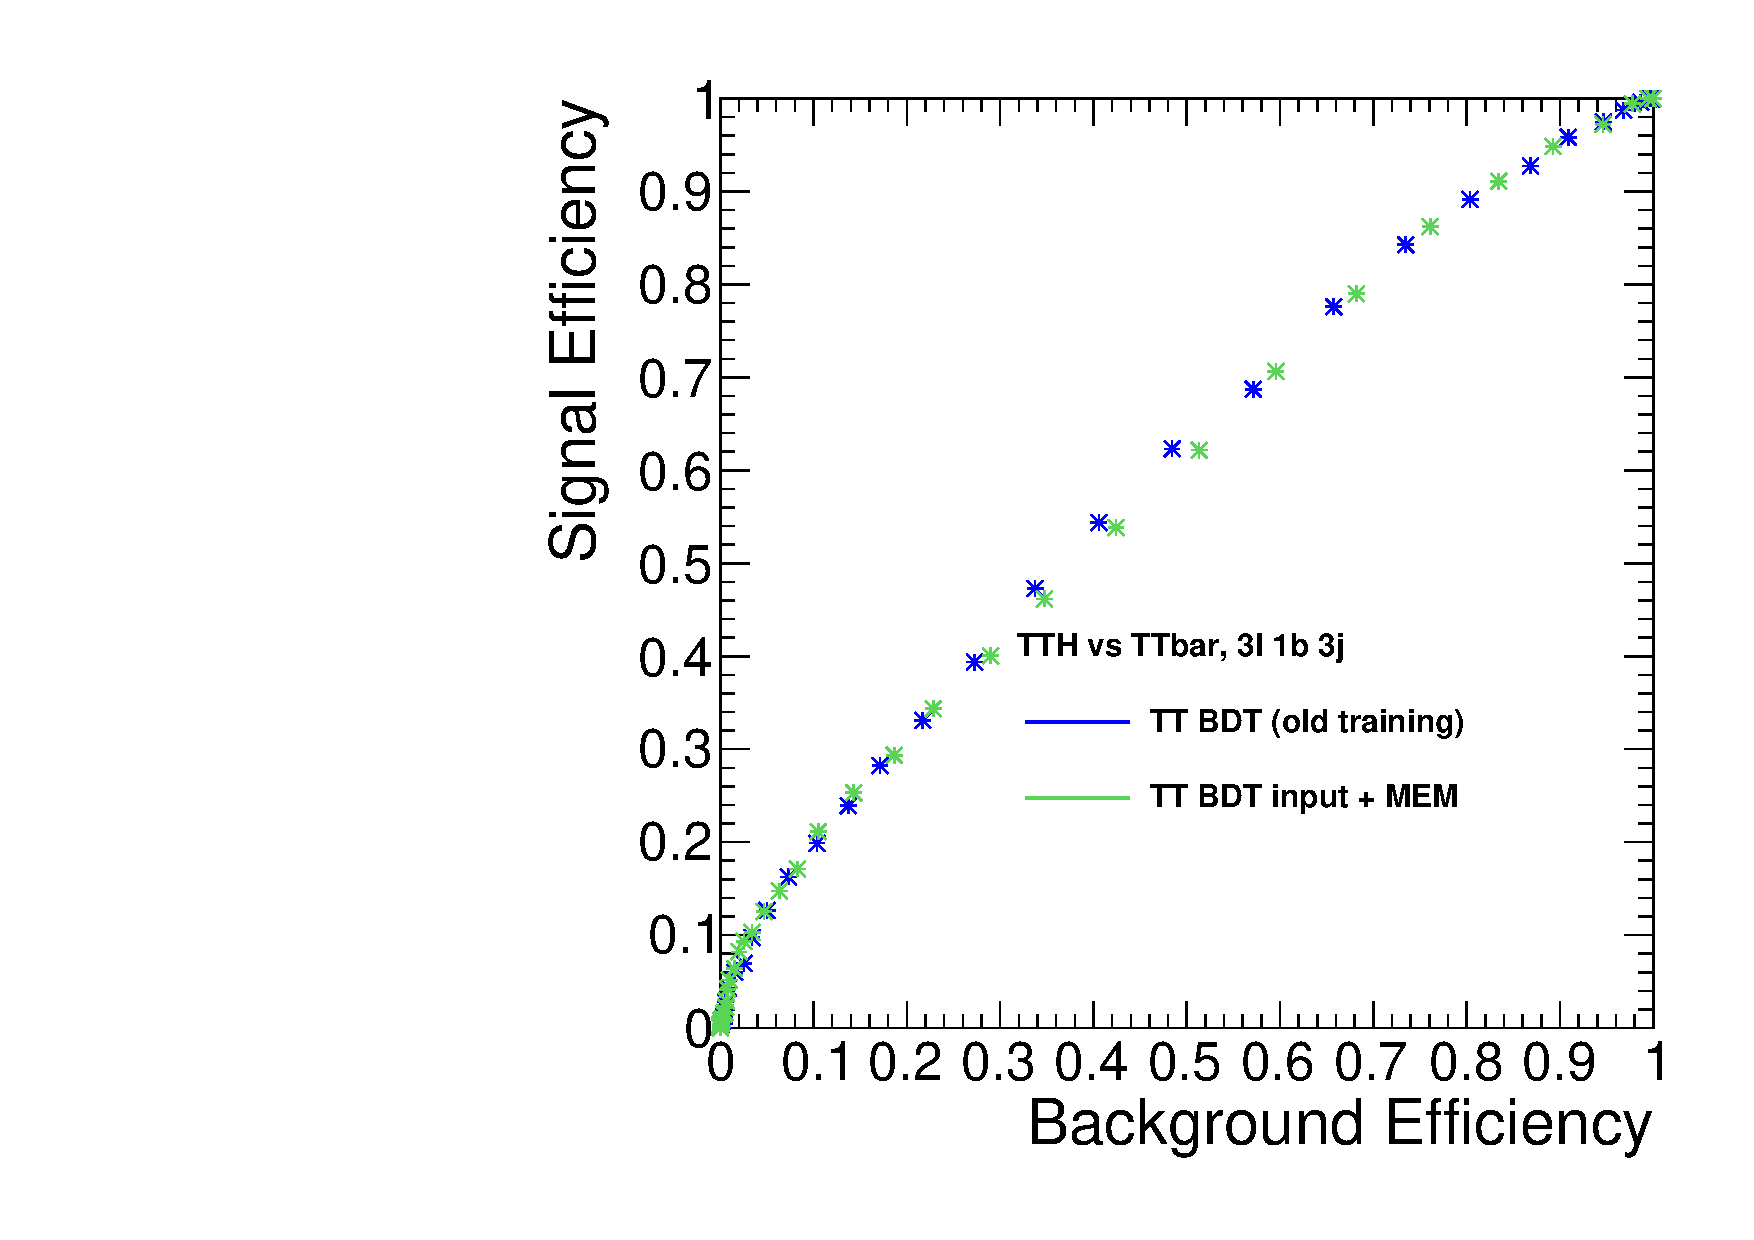
\includegraphics[width=0.4\textwidth]{plots_mem/Moriond2017/TTbar/CompareBDT_3l_1b_3j.pdf}
   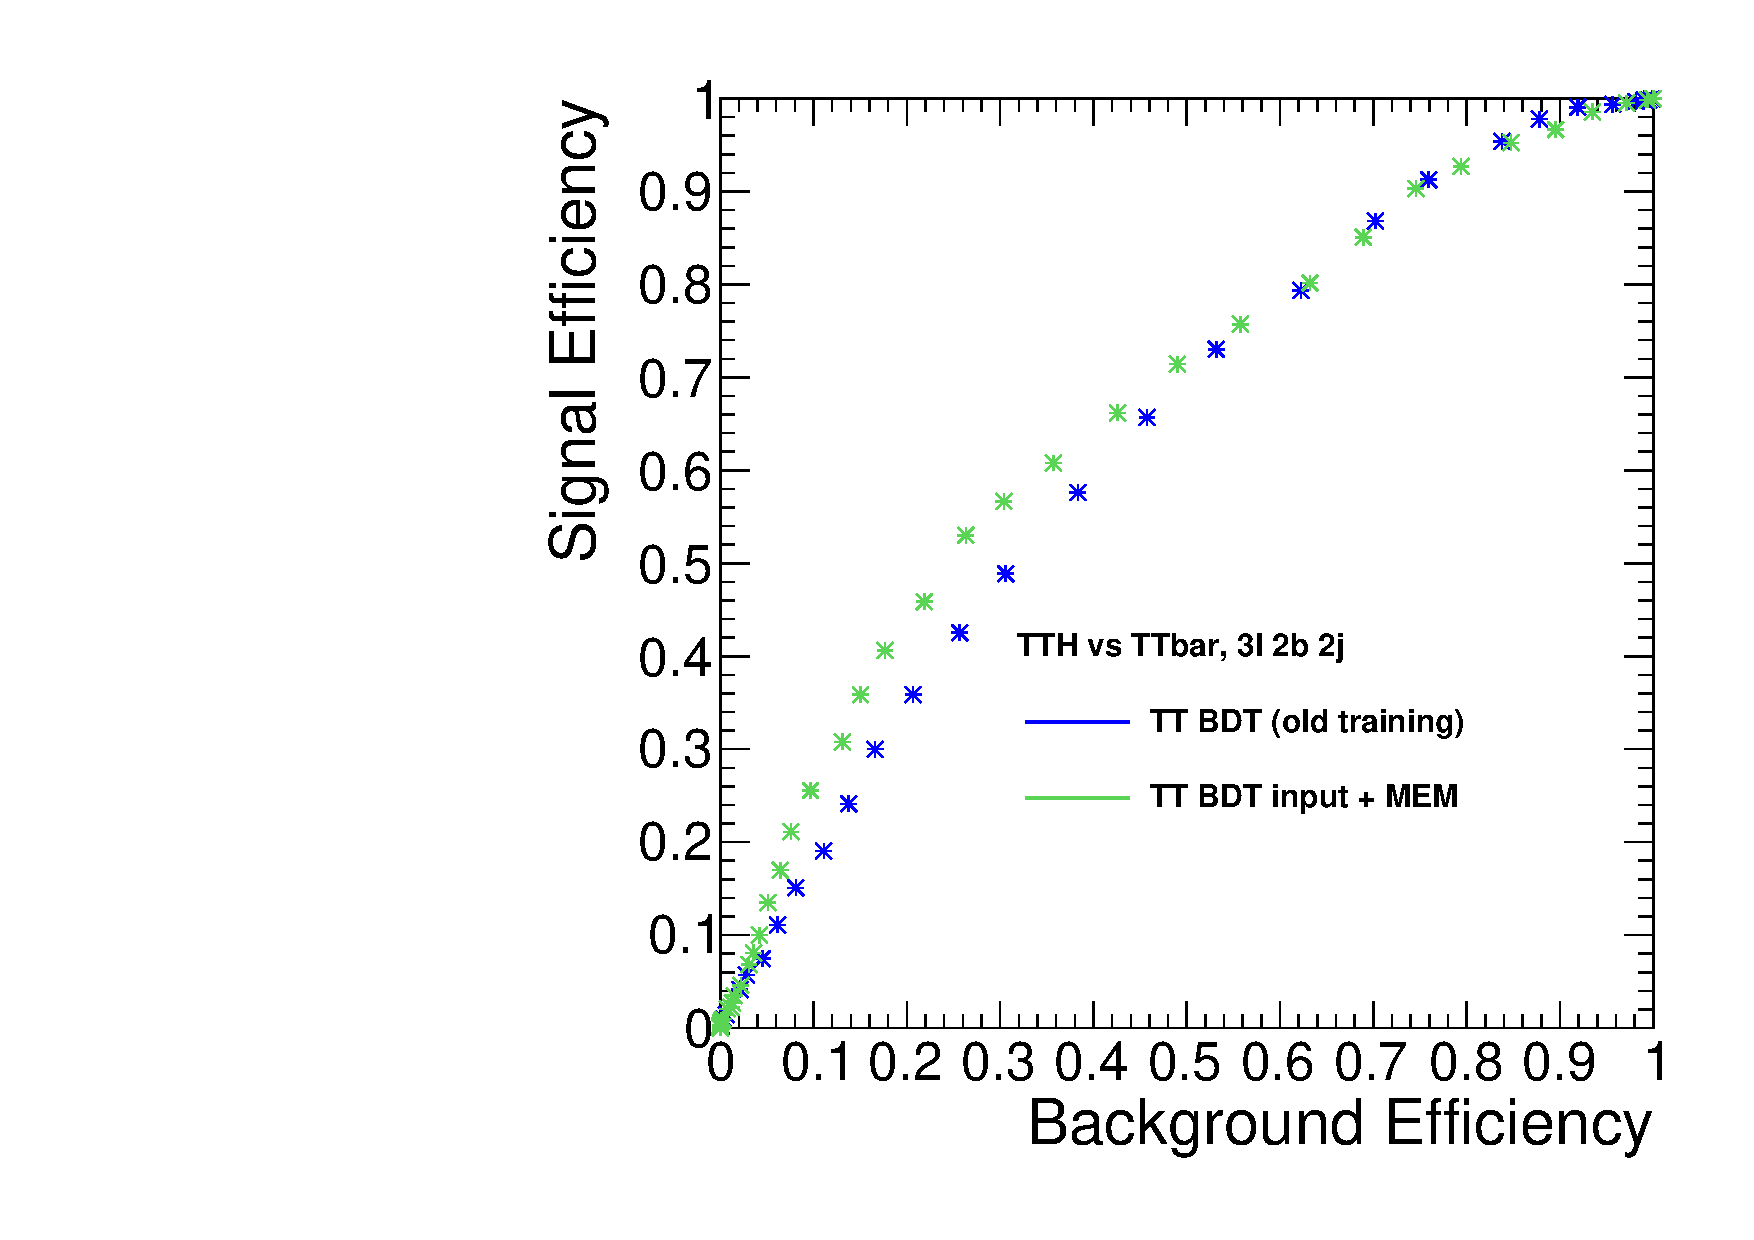
\includegraphics[width=0.4\textwidth]{plots_mem/Moriond2017/TTbar/CompareBDT_3l_2b_2j.pdf} \\
   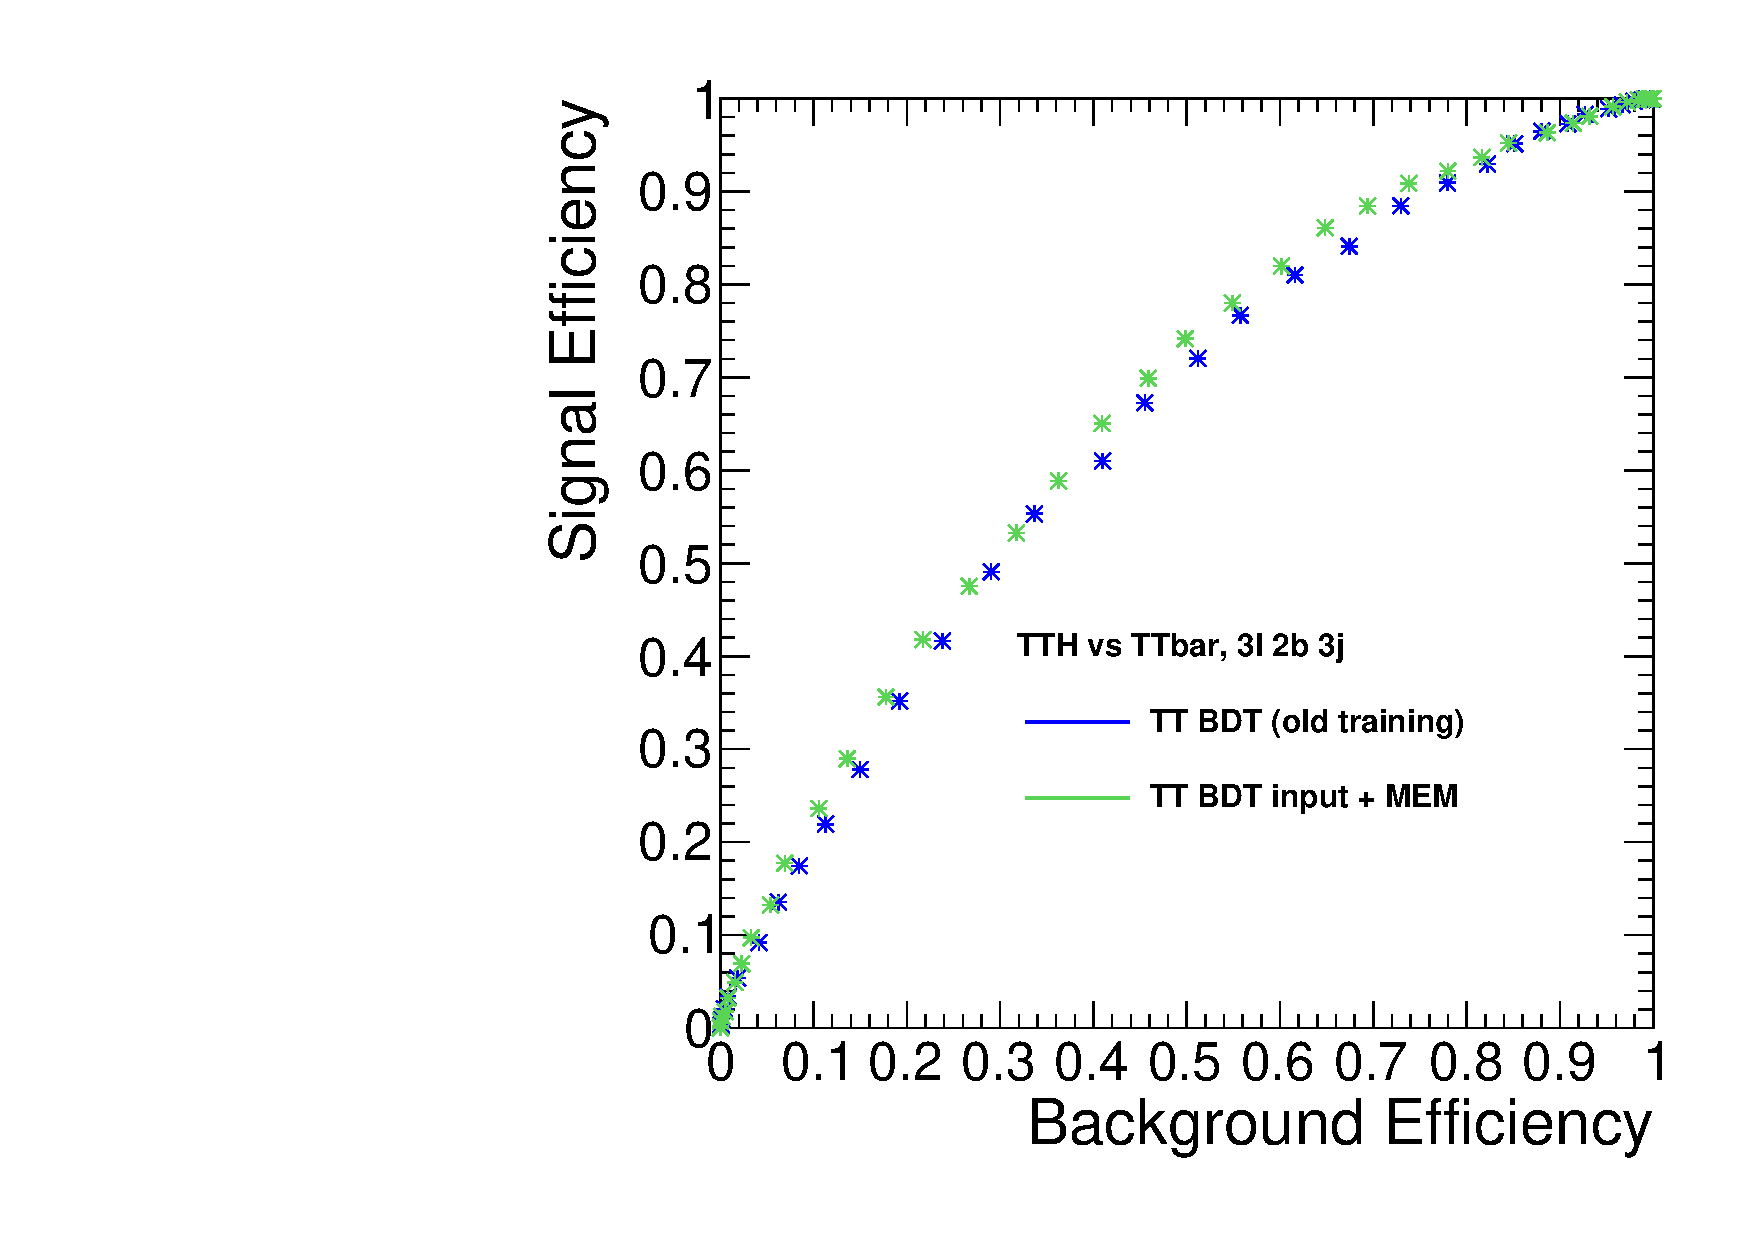
\includegraphics[width=0.4\textwidth]{plots_mem/Moriond2017/TTbar/CompareBDT_3l_2b_3j.pdf}
   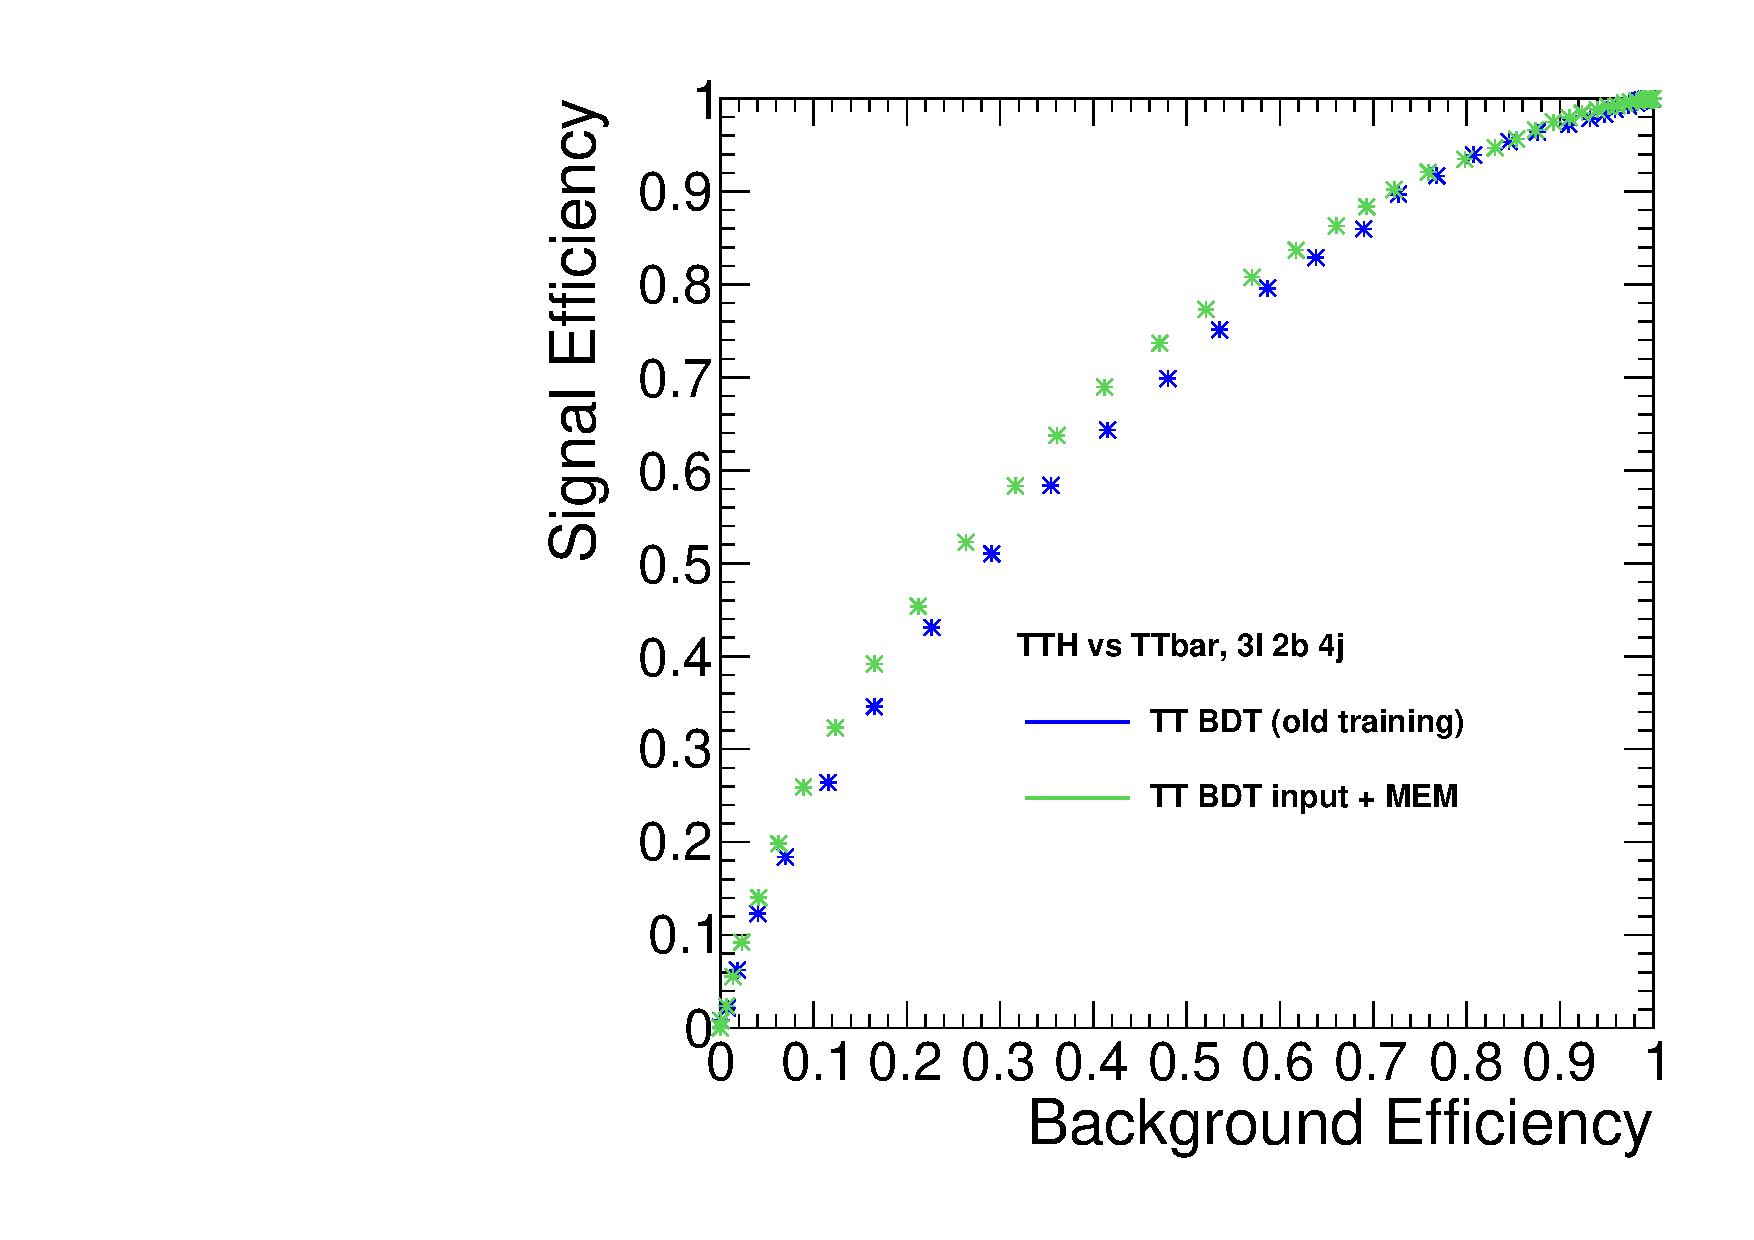
\includegraphics[width=0.4\textwidth]{plots_mem/Moriond2017/TTbar/CompareBDT_3l_2b_4j.pdf}
    \caption{ \textcolor{green}{Updated} Comparison of TT BDT and new BDT including MEM in 3l signal region for (a) all events (b) 0 missing jets, (c) 1 missing jets, (d) 2 missing jets.}
  \label{mem:BDTMEMtraining3lnoSFOS}
\end{figure}

\begin{figure}[Htb]
 \centering
   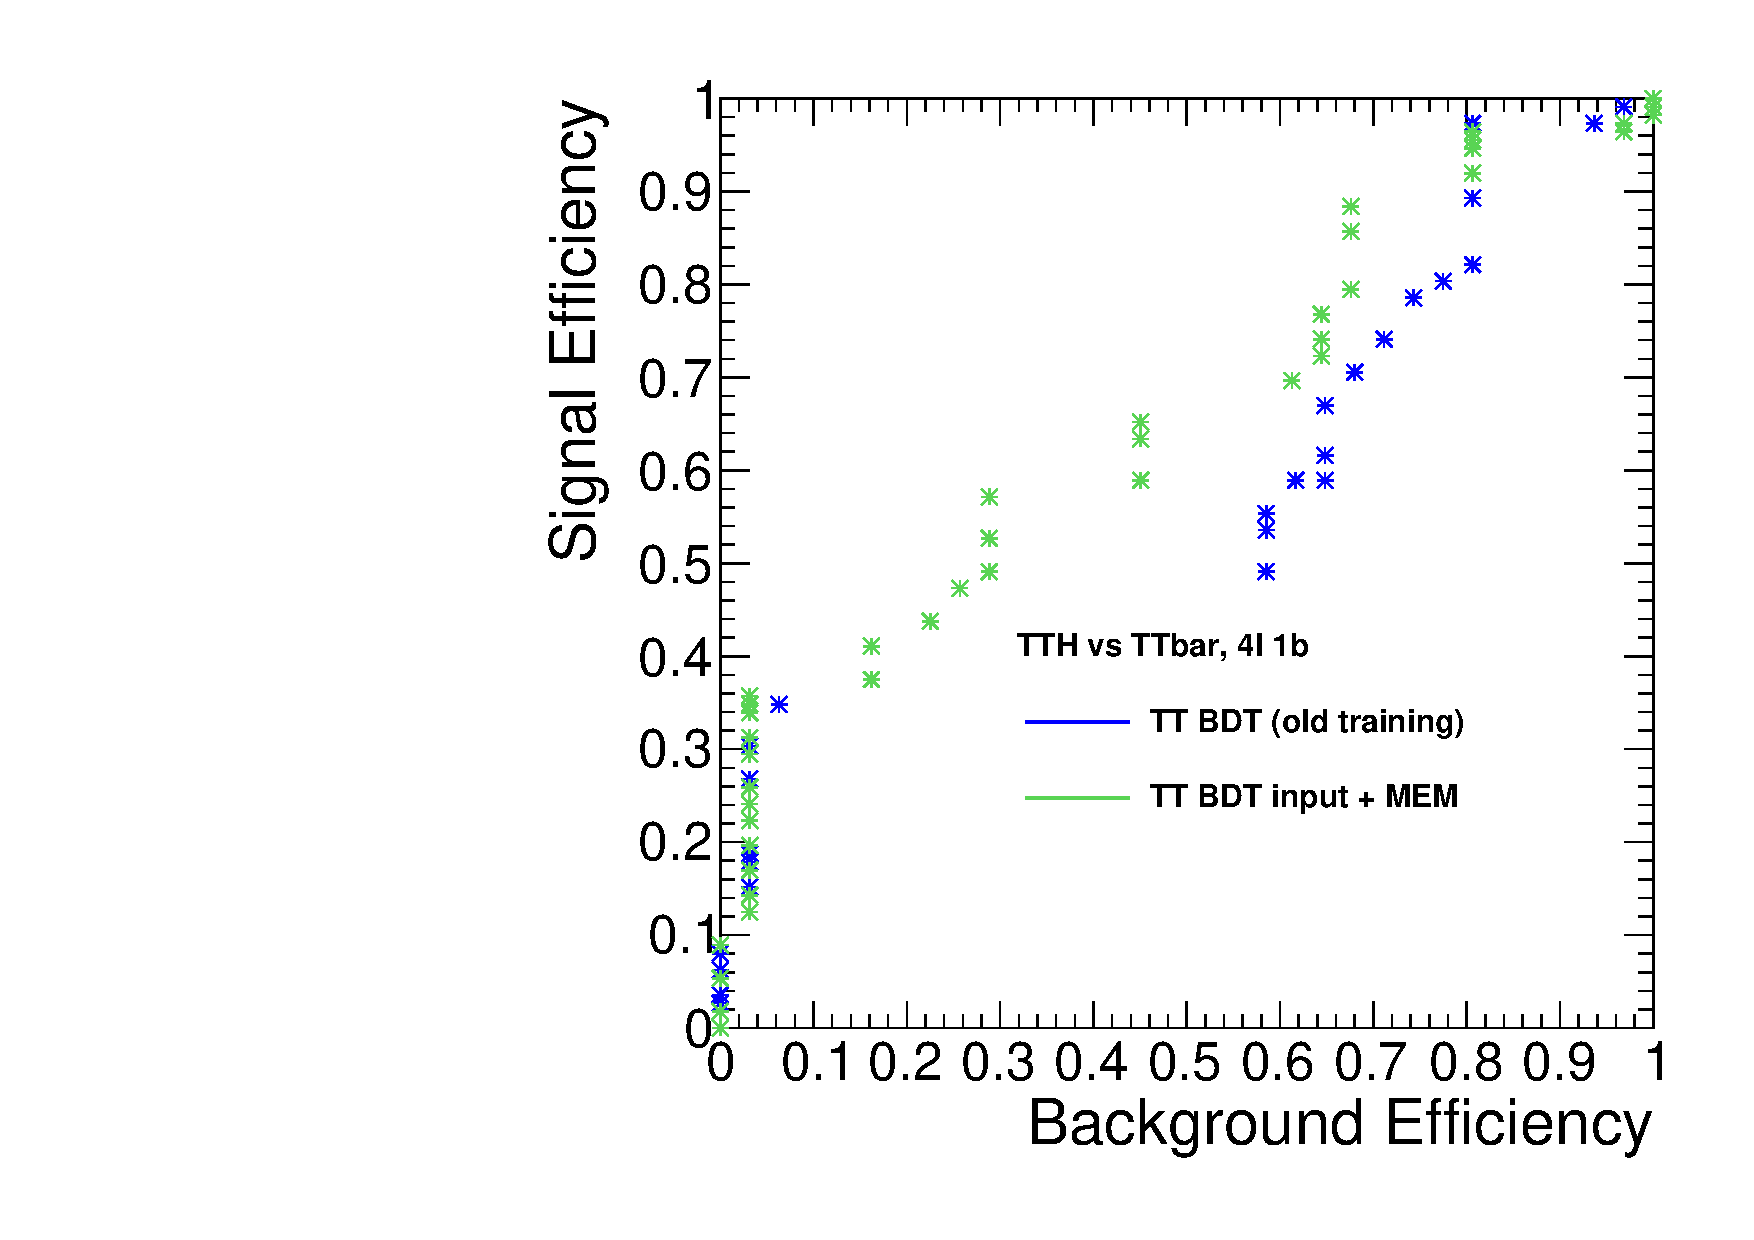
\includegraphics[width=0.4\textwidth]{plots_mem/Moriond2017/TTbar/CompareBDT_TT_1b_4l.pdf}
   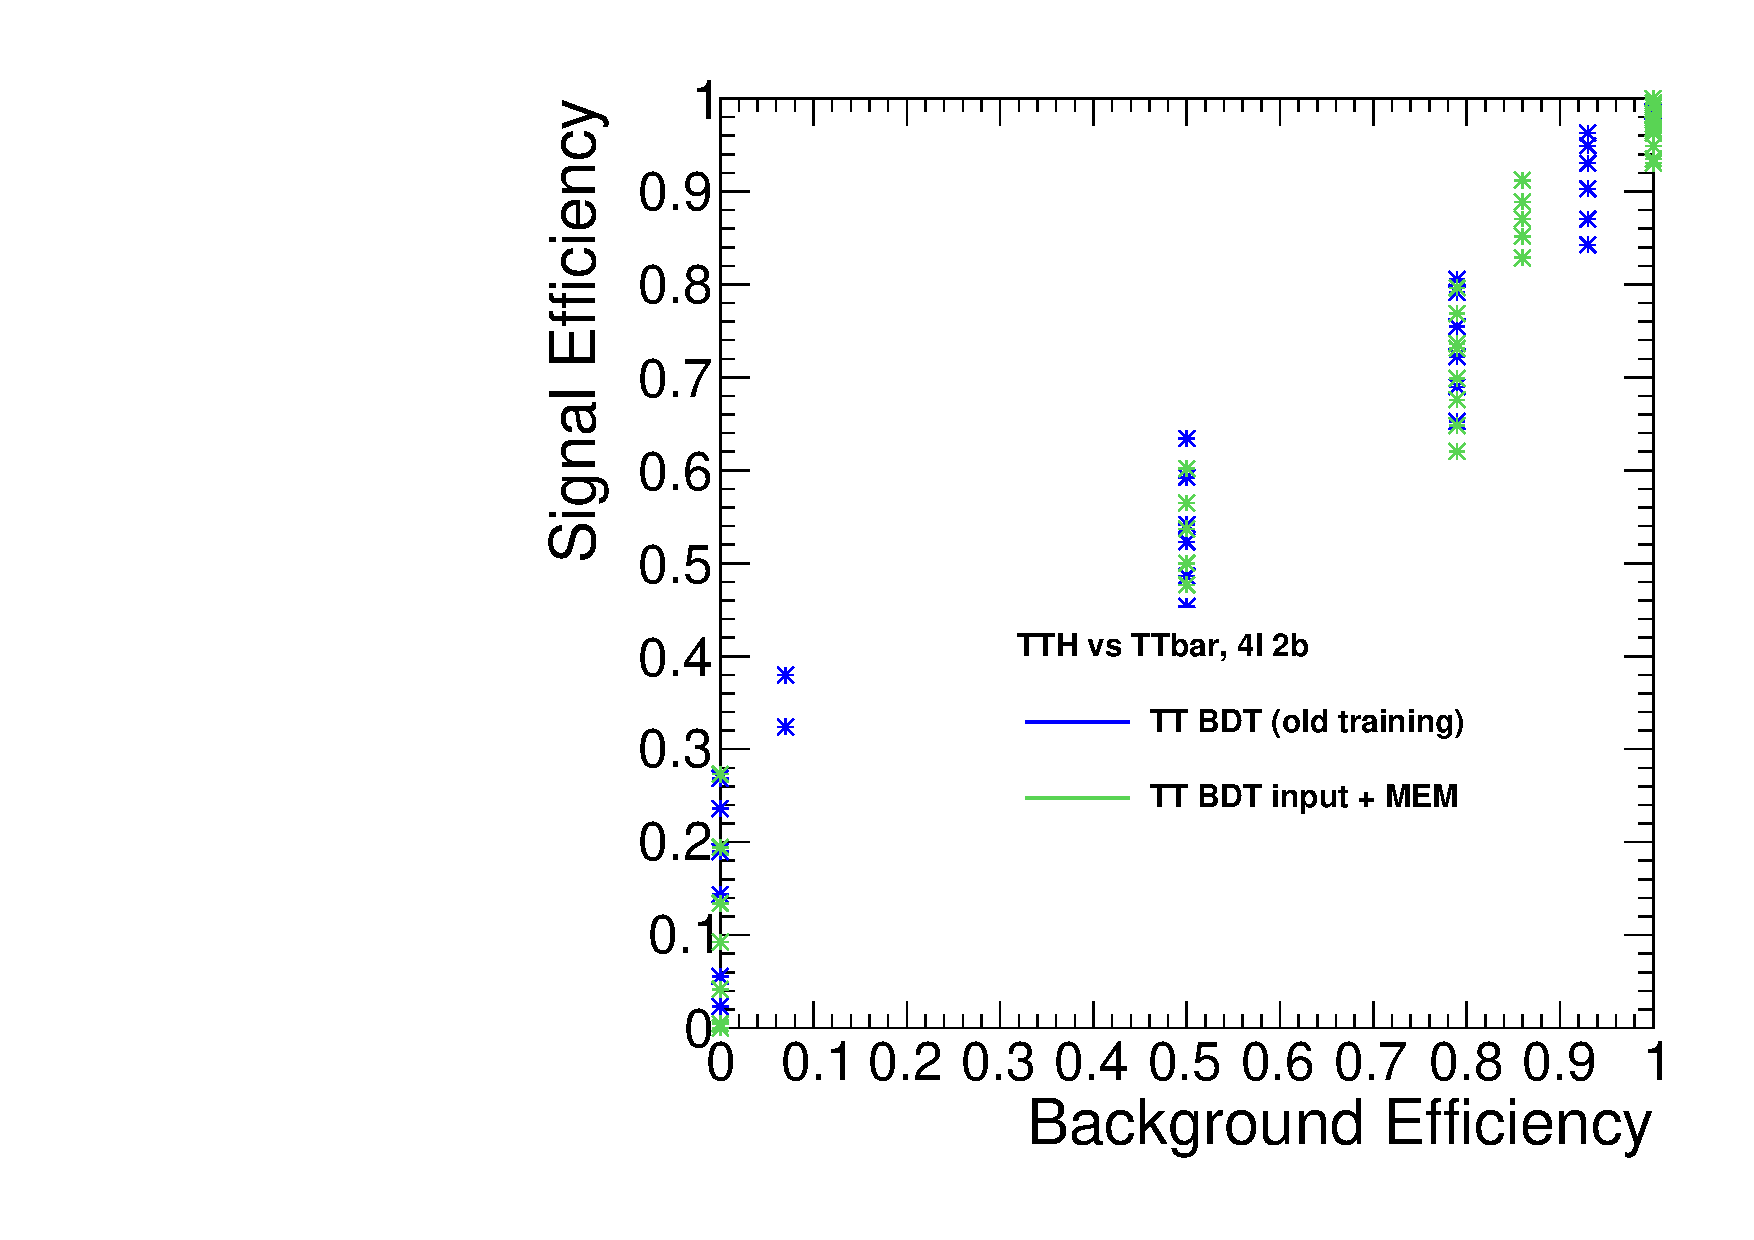
\includegraphics[width=0.4\textwidth]{plots_mem/Moriond2017/TTbar/CompareBDT_TT_2b_4l.pdf}
   \caption{ \textcolor{green}{Updated} Comparison of TT BDT and new BDT including MEM in 4l signal region for (a) 1b events, (b) 2b events}
  \label{mem:BDTMEMtraining4l}
\end{figure}

\subsection{MEM distributions after event selection}

Figures~\ref{mem:SR} and \ref{mem:AR} show the distribution of log of MEM amplitudes after the full 3l event selection, in the signal and in the lepton MVA sideband region.

\begin{figure}[Htb]
 \centering
   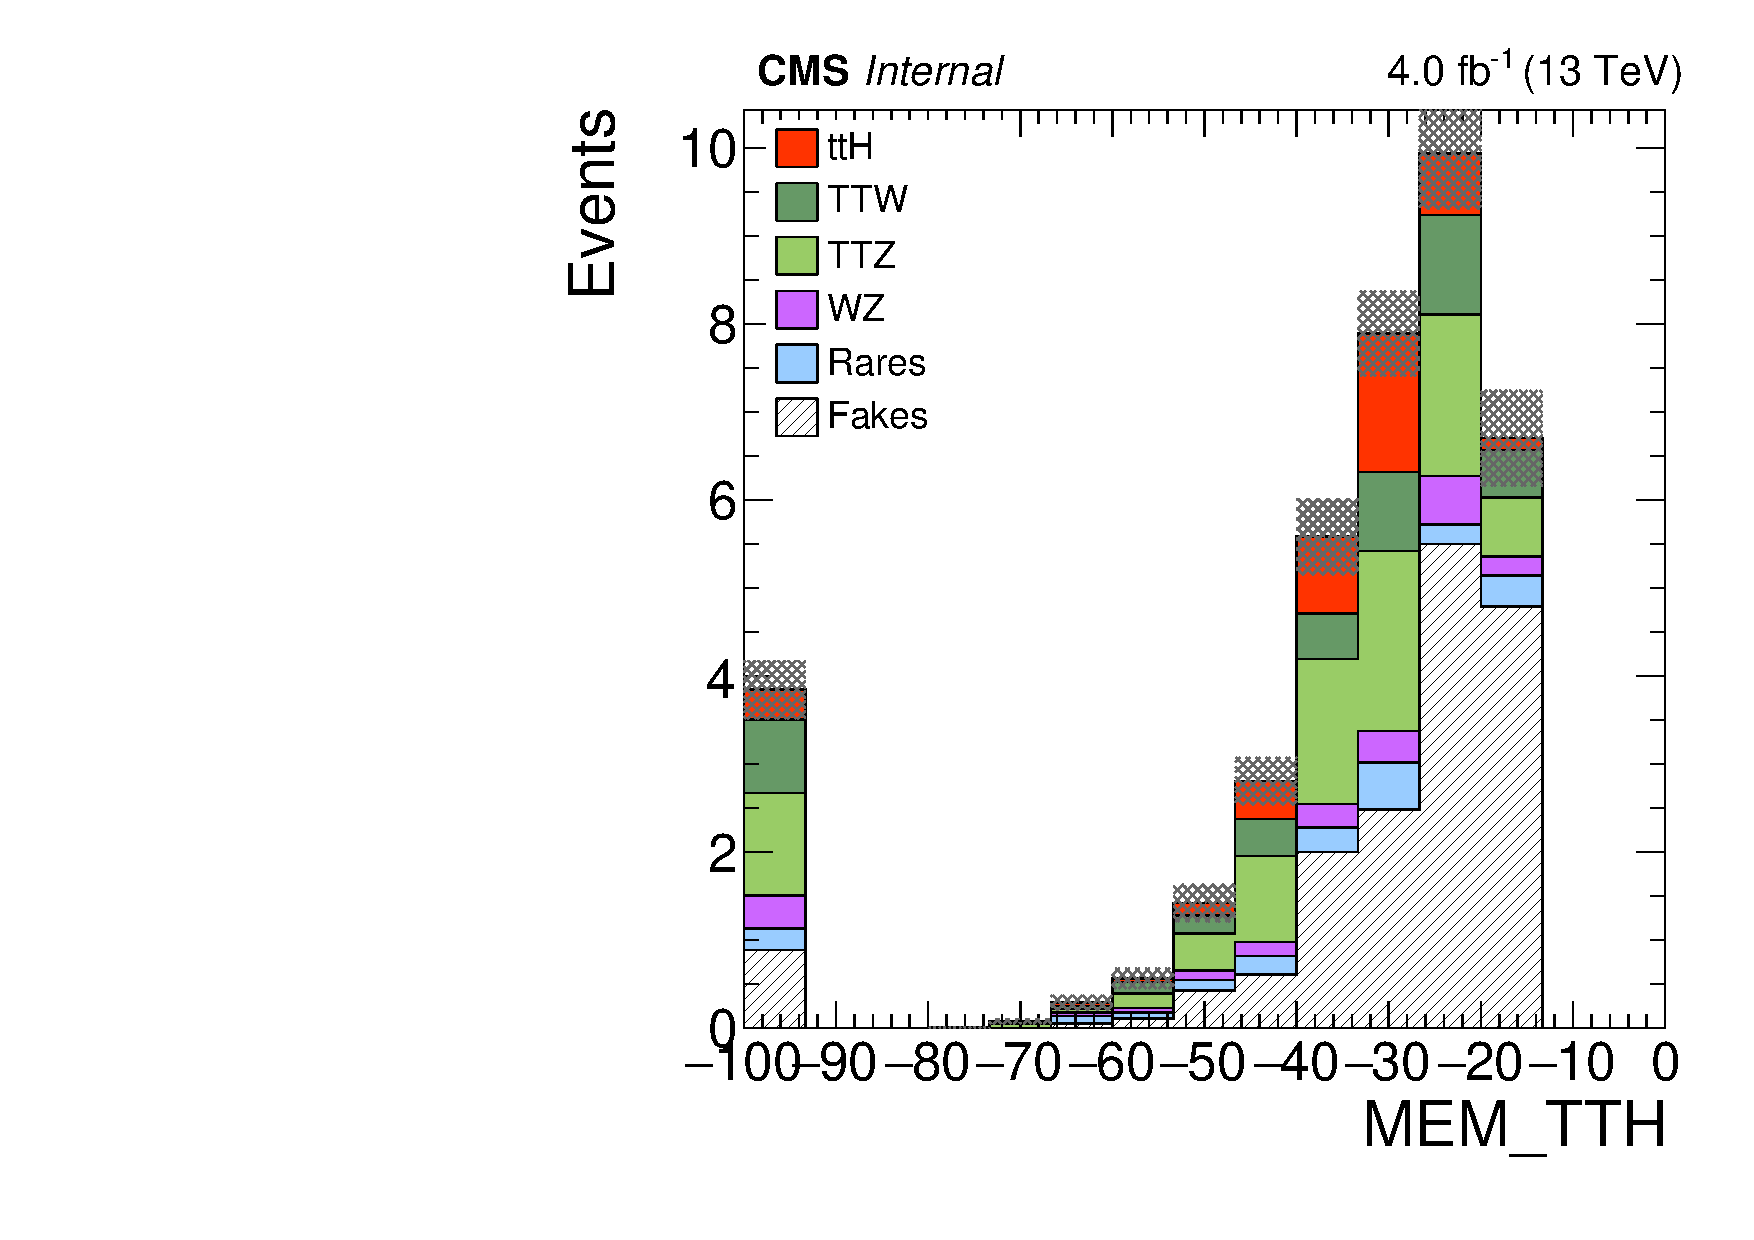
\includegraphics[width=0.32\textwidth]{plots_mem/SR/kinMVA_input_MEM_TTH}
   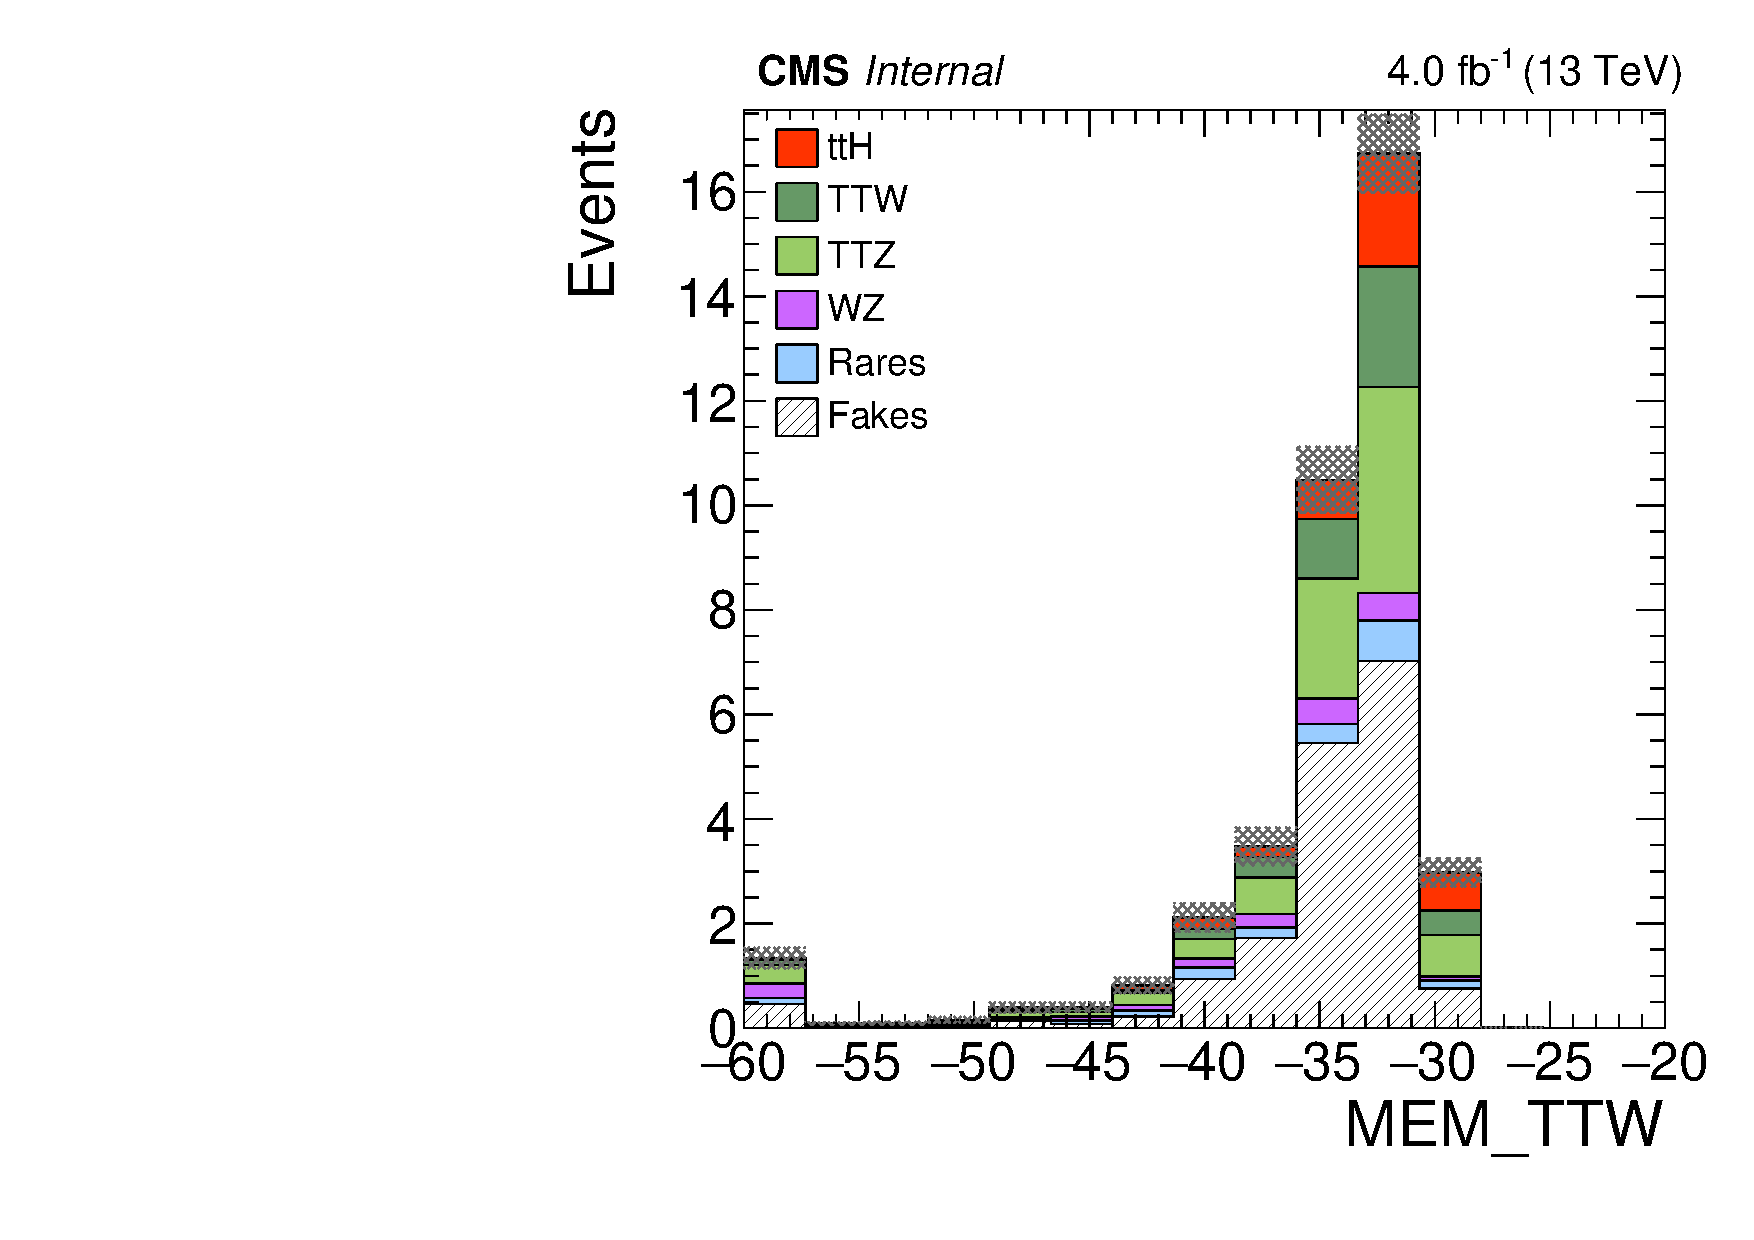
\includegraphics[width=0.32\textwidth]{plots_mem/SR/kinMVA_input_MEM_TTW}
   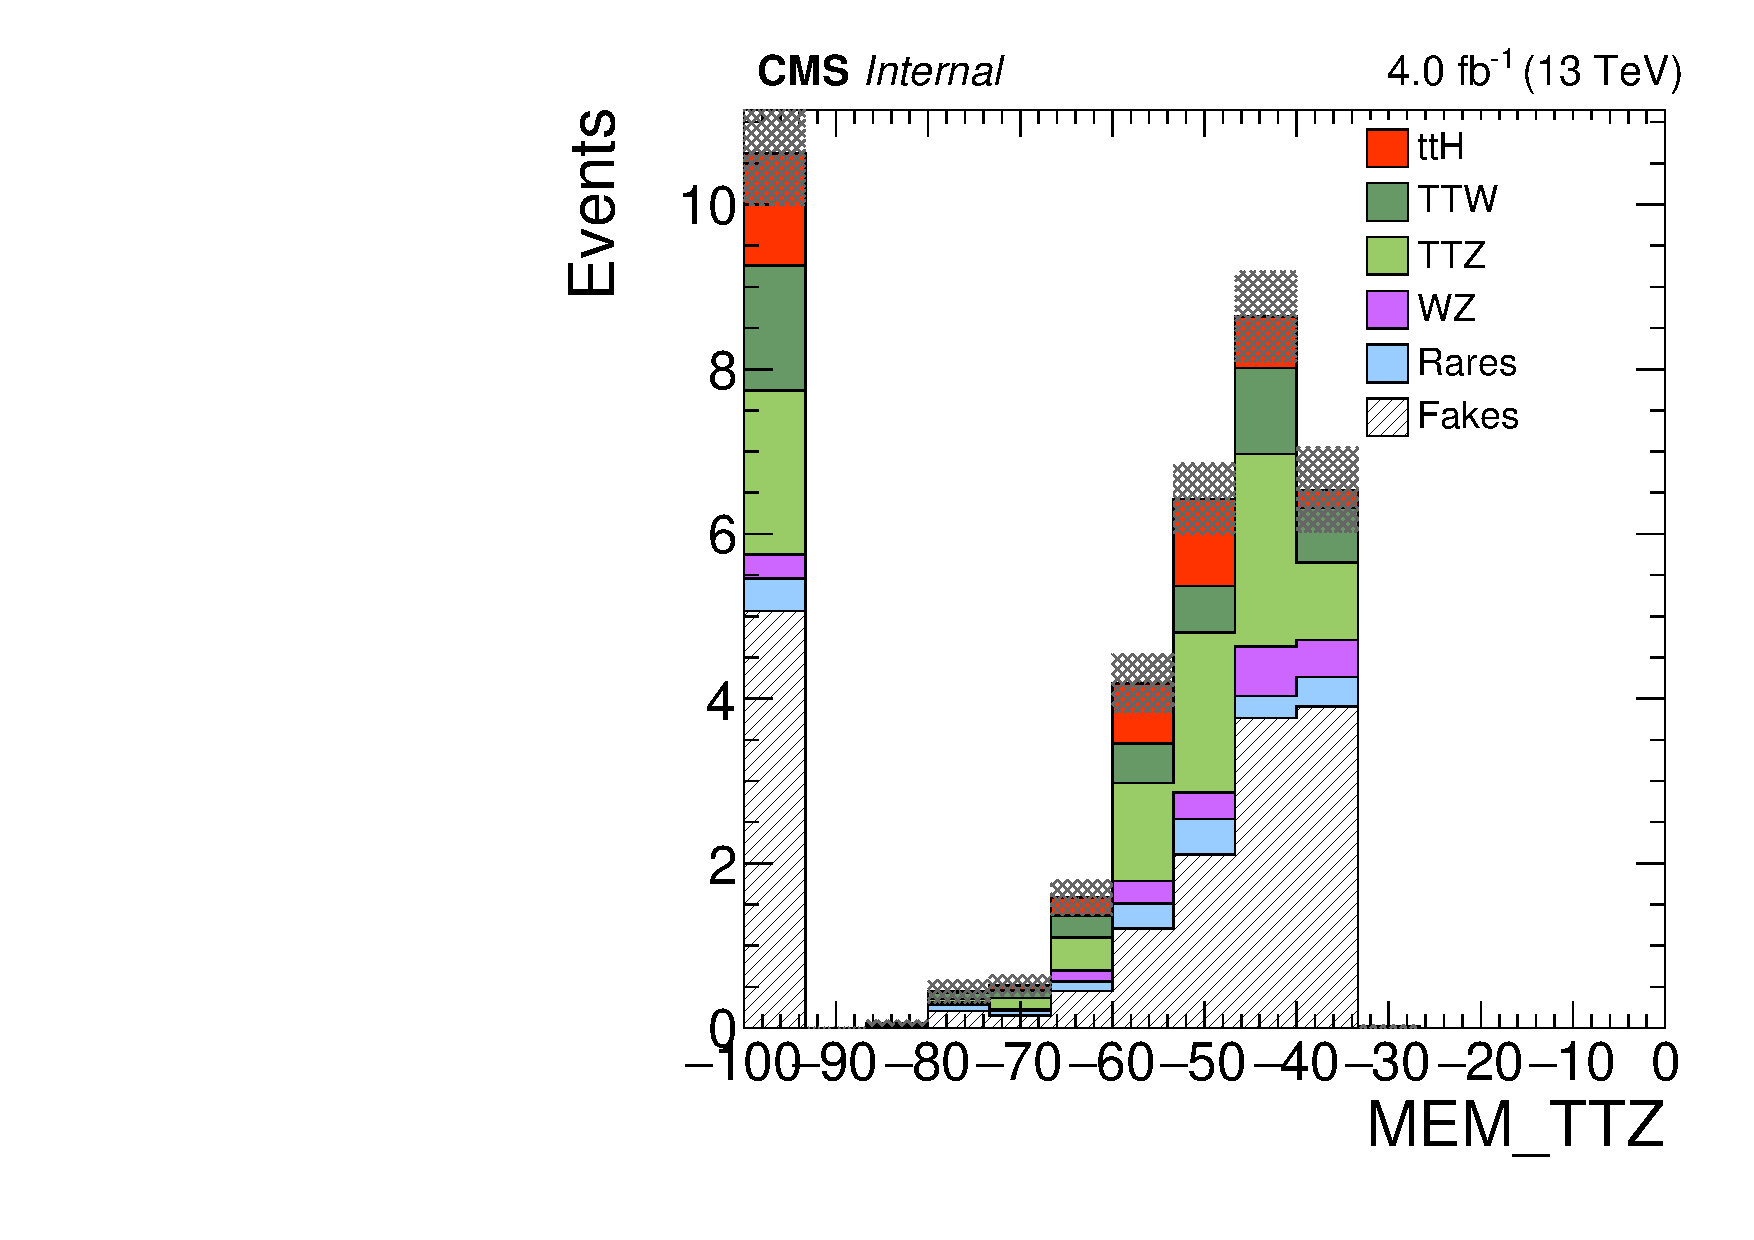
\includegraphics[width=0.32\textwidth]{plots_mem/SR/kinMVA_input_MEM_TTZ}
   \caption{Log of MEM weights in the 3l signal region.}
  \label{mem:SR}
\end{figure}

\begin{figure}[Htb]
 \centering
   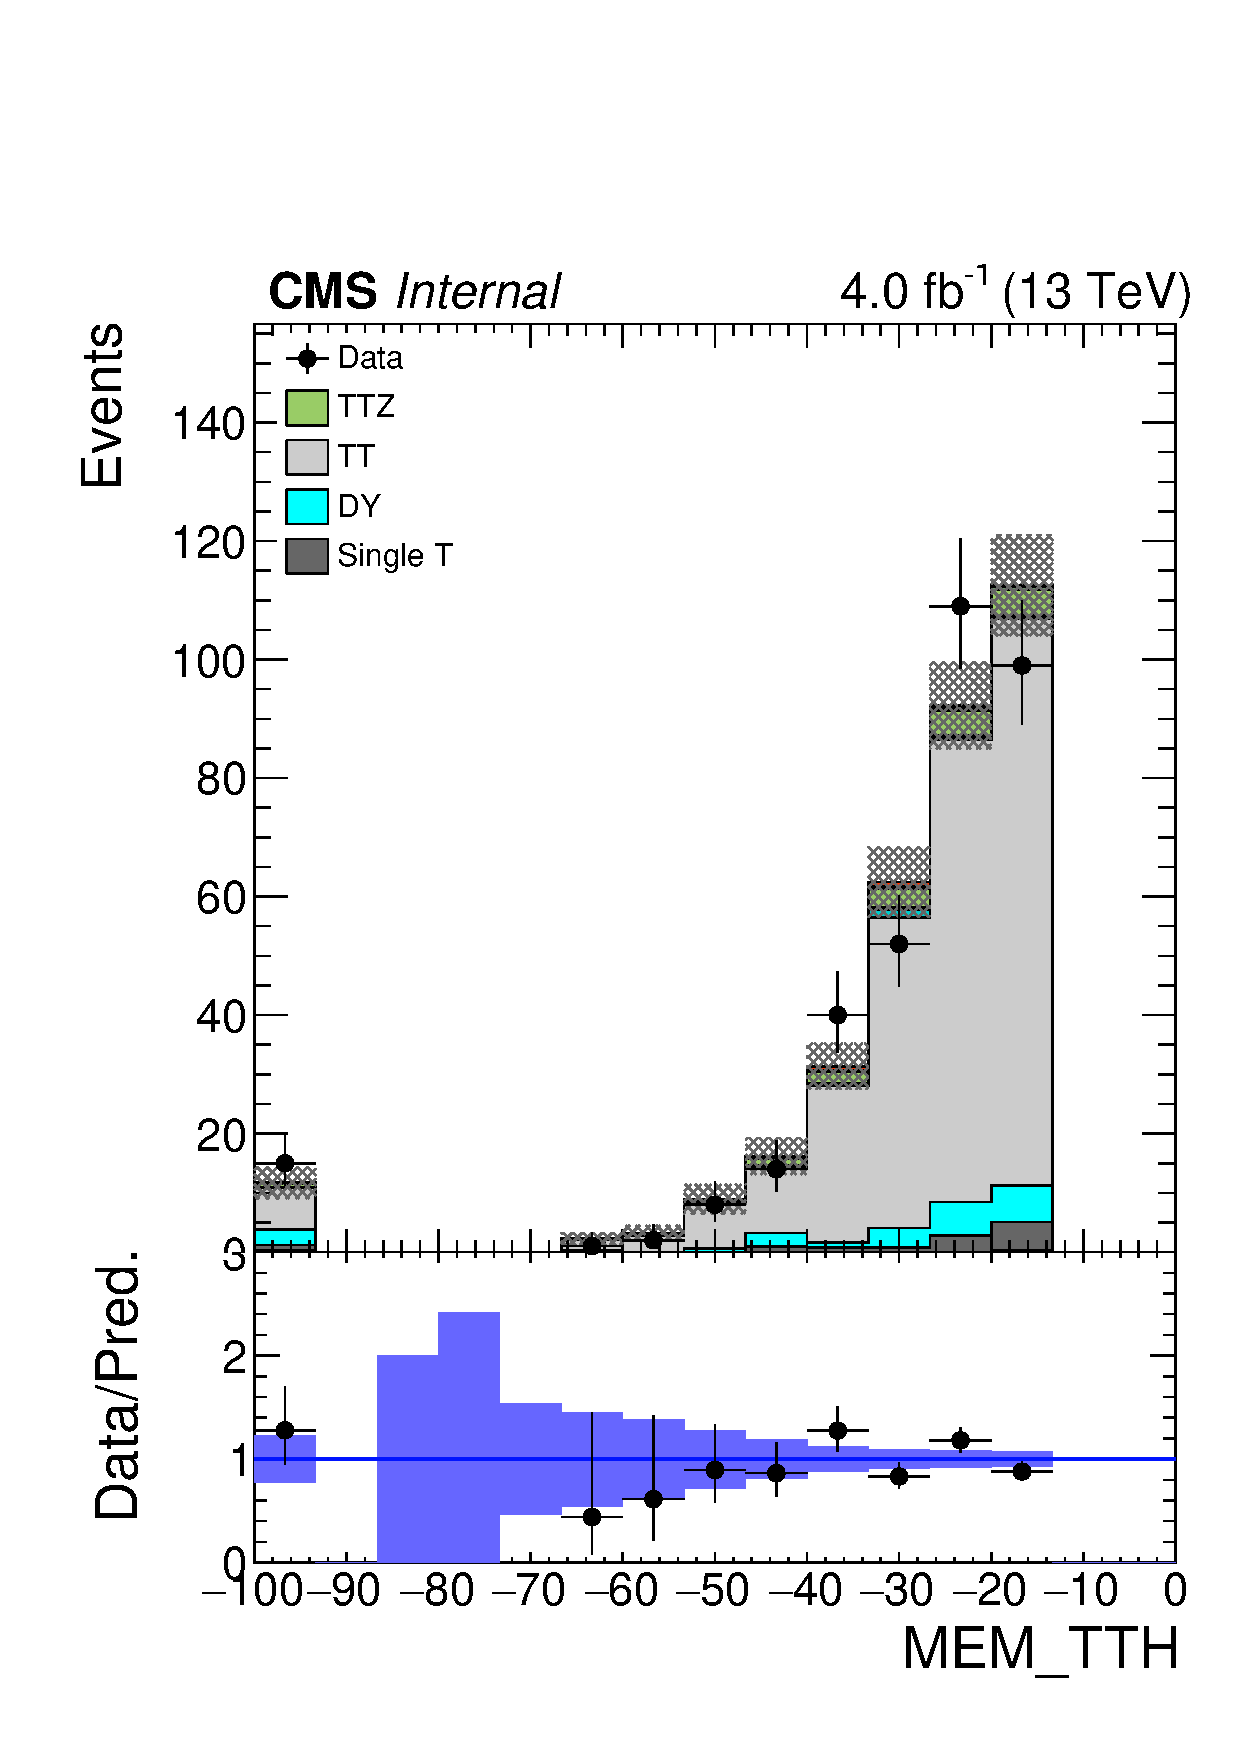
\includegraphics[width=0.32\textwidth]{plots_mem/Appl/kinMVA_input_MEM_TTH}
   \includegraphics[width=0.32\textwidth]{plots_mem/Appl/kinMVA_input_MEM_TTW}
   \includegraphics[width=0.32\textwidth]{plots_mem/Appl/kinMVA_input_MEM_TTZ}
   \caption{Log of MEM weights in the 3l application region.}
  \label{mem:AR}
\end{figure}
